%DIF 1-44d1
%DIF LATEXDIFF DIFFERENCE FILE
%DIF DEL /var/folders/ph/r5fc9nzd1j38q4j50kgwd4cw0000gn/T/kd9B6KjoQ5/latexdiff-vc-ce3856c6/ms/LMAms_main.tex   Mon Sep  5 18:45:08 2022
%DIF ADD ms/LMAms_main.tex                                                                                     Fri Mar 31 10:29:05 2023
%DIF < %%
%DIF < % Copyright (c) 2017 - 2020, Pascal Wagler;
%DIF < % Copyright (c) 2014 - 2020, John MacFarlane
%DIF < %
%DIF < % All rights reserved.
%DIF < %
%DIF < % Redistribution and use in source and binary forms, with or without
%DIF < % modification, are permitted provided that the following conditions
%DIF < % are met:
%DIF < %
%DIF < % - Redistributions of source code must retain the above copyright
%DIF < % notice, this list of conditions and the following disclaimer.
%DIF < %
%DIF < % - Redistributions in binary form must reproduce the above copyright
%DIF < % notice, this list of conditions and the following disclaimer in the
%DIF < % documentation and/or other materials provided with the distribution.
%DIF < %
%DIF < % - Neither the name of John MacFarlane nor the names of other
%DIF < % contributors may be used to endorse or promote products derived
%DIF < % from this software without specific prior written permission.
%DIF < %
%DIF < % THIS SOFTWARE IS PROVIDED BY THE COPYRIGHT HOLDERS AND CONTRIBUTORS
%DIF < % "AS IS" AND ANY EXPRESS OR IMPLIED WARRANTIES, INCLUDING, BUT NOT
%DIF < % LIMITED TO, THE IMPLIED WARRANTIES OF MERCHANTABILITY AND FITNESS
%DIF < % FOR A PARTICULAR PURPOSE ARE DISCLAIMED. IN NO EVENT SHALL THE
%DIF < % COPYRIGHT OWNER OR CONTRIBUTORS BE LIABLE FOR ANY DIRECT, INDIRECT,
%DIF < % INCIDENTAL, SPECIAL, EXEMPLARY, OR CONSEQUENTIAL DAMAGES (INCLUDING,
%DIF < % BUT NOT LIMITED TO, PROCUREMENT OF SUBSTITUTE GOODS OR SERVICES;
%DIF < % LOSS OF USE, DATA, OR PROFITS; OR BUSINESS INTERRUPTION) HOWEVER
%DIF < % CAUSED AND ON ANY THEORY OF LIABILITY, WHETHER IN CONTRACT, STRICT
%DIF < % LIABILITY, OR TORT (INCLUDING NEGLIGENCE OR OTHERWISE) ARISING IN
%DIF < % ANY WAY OUT OF THE USE OF THIS SOFTWARE, EVEN IF ADVISED OF THE
%DIF < % POSSIBILITY OF SUCH DAMAGE.
%DIF < %%
%DIF < 
%DIF < %%
%DIF < % This is the Eisvogel pandoc LaTeX template.
%DIF < %
%DIF < % For usage information and examples visit the official GitHub page:
%DIF < % https://github.com/Wandmalfarbe/pandoc-latex-template
%DIF < %%
%DIF < 
%DIF < \DeclareUnicodeCharacter{2212}{-}
%DIF < 
%DIF -------
% Options for packages loaded elsewhere
\PassOptionsToPackage{unicode}{hyperref}
\PassOptionsToPackage{hyphens}{url}
%DIF 48c4
%DIF < \PassOptionsToPackage{dvipsnames,svgnames*,x11names*,table}{xcolor}
%DIF -------
\PassOptionsToPackage{dvipsnames,svgnames,x11names}{xcolor} %DIF > 
%DIF -------
%
\documentclass[
  12pt,
%DIF 52-54c8-12
%DIF <   a4paper,
%DIF < ,tablecaptionabove
%DIF < ]{scrartcl}
%DIF -------
  letterpaper, %DIF > 
  DIV=11, %DIF > 
  numbers=noendperiod]{scrartcl} %DIF > 
 %DIF > 
\usepackage{amsmath,amssymb} %DIF > 
%DIF -------
\usepackage{lmodern}
%DIF 56-60c14-15
%DIF < \usepackage{setspace}
%DIF < \setstretch{1.2}
%DIF < \usepackage{amssymb,amsmath}
%DIF < \usepackage{ifxetex,ifluatex}
%DIF < \ifnum 0\ifxetex 1\fi\ifluatex 1\fi=0 % if pdftex
%DIF -------
\usepackage{iftex} %DIF > 
\ifPDFTeX %DIF > 
%DIF -------
  \usepackage[T1]{fontenc}
  \usepackage[utf8]{inputenc}
  \usepackage{textcomp} % provide euro and other symbols
\else % if luatex or xetex
  \usepackage{unicode-math}
  \defaultfontfeatures{Scale=MatchLowercase}
  \defaultfontfeatures[\rmfamily]{Ligatures=TeX,Scale=1}
\fi
% Use upquote if available, for straight quotes in verbatim environments
\IfFileExists{upquote.sty}{\usepackage{upquote}}{}
\IfFileExists{microtype.sty}{% use microtype if available
  \usepackage[]{microtype}
  \UseMicrotypeSet[protrusion]{basicmath} % disable protrusion for tt fonts
}{}
\makeatletter
\@ifundefined{KOMAClassName}{% if non-KOMA class
  \IfFileExists{parskip.sty}{%
    \usepackage{parskip}
  }{% else
    \setlength{\parindent}{0pt}
    \setlength{\parskip}{6pt plus 2pt minus 1pt}}
}{% if KOMA class
  \KOMAoptions{parskip=half}}
\makeatother
\usepackage{xcolor}
%DIF 86-100d41
%DIF < \definecolor{default-linkcolor}{HTML}{A50000}
%DIF < \definecolor{default-filecolor}{HTML}{A50000}
%DIF < \definecolor{default-citecolor}{HTML}{4077C0}
%DIF < \definecolor{default-urlcolor}{HTML}{4077C0}
%DIF < \IfFileExists{xurl.sty}{\usepackage{xurl}}{} % add URL line breaks if available
%DIF < \IfFileExists{bookmark.sty}{\usepackage{bookmark}}{\usepackage{hyperref}}
%DIF < \hypersetup{
%DIF <   colorlinks=true,
%DIF <   linkcolor=blue,
%DIF <   filecolor=default-filecolor,
%DIF <   citecolor=default-citecolor,
%DIF <   urlcolor=default-urlcolor,
%DIF <   breaklinks=true,
%DIF <   pdfcreator={LaTeX via pandoc with the Eisvogel template}}
%DIF < \urlstyle{same} % disable monospaced font for URLs
%DIF -------
\usepackage[margin=1in]{geometry}
%DIF 102c42-57
%DIF < \usepackage{longtable,booktabs}
%DIF -------
\setlength{\emergencystretch}{3em} % prevent overfull lines %DIF > 
\setcounter{secnumdepth}{-\maxdimen} % remove section numbering %DIF > 
% Make \paragraph and \subparagraph free-standing %DIF > 
\ifx\paragraph\undefined\else %DIF > 
  \let\oldparagraph\paragraph %DIF > 
  \renewcommand{\paragraph}[1]{\oldparagraph{#1}\mbox{}} %DIF > 
\fi %DIF > 
\ifx\subparagraph\undefined\else %DIF > 
  \let\oldsubparagraph\subparagraph %DIF > 
  \renewcommand{\subparagraph}[1]{\oldsubparagraph{#1}\mbox{}} %DIF > 
\fi %DIF > 
 %DIF > 
 %DIF > 
\providecommand{\tightlist}{% %DIF > 
  \setlength{\itemsep}{0pt}\setlength{\parskip}{0pt}}\usepackage{longtable,booktabs,array} %DIF > 
\usepackage{calc} % for calculating minipage widths %DIF > 
%DIF -------
% Correct order of tables after \paragraph or \subparagraph
\usepackage{etoolbox}
\makeatletter
\patchcmd\longtable{\par}{\if@noskipsec\mbox{}\fi\par}{}{}
\makeatother
% Allow footnotes in longtable head/foot
\IfFileExists{footnotehyper.sty}{\usepackage{footnotehyper}}{\usepackage{footnote}}
\makesavenoteenv{longtable}
%DIF 111-112d66
%DIF < % add backlinks to footnote references, cf. https://tex.stackexchange.com/questions/302266/make-footnote-clickable-both-ways
%DIF < \usepackage{footnotebackref}
%DIF -------
\usepackage{graphicx}
\makeatletter
\def\maxwidth{\ifdim\Gin@nat@width>\linewidth\linewidth\else\Gin@nat@width\fi}
\def\maxheight{\ifdim\Gin@nat@height>\textheight\textheight\else\Gin@nat@height\fi}
\makeatother
% Scale images if necessary, so that they will not overflow the page
% margins by default, and it is still possible to overwrite the defaults
% using explicit options in \includegraphics[width, height, ...]{}
\setkeys{Gin}{width=\maxwidth,height=\maxheight,keepaspectratio}
%DIF 122-129c75-91
%DIF < \setlength{\emergencystretch}{3em}  % prevent overfull lines
%DIF < \providecommand{\tightlist}{%
%DIF <   \setlength{\itemsep}{0pt}\setlength{\parskip}{0pt}}
%DIF < \setcounter{secnumdepth}{-\maxdimen} % remove section numbering
%DIF < % Make \paragraph and \subparagraph free-standing
%DIF < \ifx\paragraph\undefined\else
%DIF <   \let\oldparagraph\paragraph
%DIF <   \renewcommand{\paragraph}[1]{\oldparagraph{#1}\mbox{}}
%DIF -------
% Set default figure placement to htbp %DIF > 
\makeatletter %DIF > 
\def\fps@figure{htbp} %DIF > 
\makeatother %DIF > 
\newlength{\cslhangindent} %DIF > 
\setlength{\cslhangindent}{1.5em} %DIF > 
\newlength{\csllabelwidth} %DIF > 
\setlength{\csllabelwidth}{3em} %DIF > 
\newlength{\cslentryspacingunit} % times entry-spacing %DIF > 
\setlength{\cslentryspacingunit}{\parskip} %DIF > 
\newenvironment{CSLReferences}[2] % #1 hanging-ident, #2 entry spacing %DIF > 
 {% don't indent paragraphs %DIF > 
  \setlength{\parindent}{0pt} %DIF > 
  % turn on hanging indent if param 1 is 1 %DIF > 
  \ifodd #1 %DIF > 
  \let\oldpar\par %DIF > 
  \def\par{\hangindent=\cslhangindent\oldpar} %DIF > 
%DIF -------
  \fi
%DIF 131-134c93-101
%DIF < \ifx\subparagraph\undefined\else
%DIF <   \let\oldsubparagraph\subparagraph
%DIF <   \renewcommand{\subparagraph}[1]{\oldsubparagraph{#1}\mbox{}}
%DIF < \fi
%DIF -------
  % set entry spacing %DIF > 
  \setlength{\parskip}{#2\cslentryspacingunit} %DIF > 
 }% %DIF > 
 {} %DIF > 
\usepackage{calc} %DIF > 
\newcommand{\CSLBlock}[1]{#1\hfill\break} %DIF > 
\newcommand{\CSLLeftMargin}[1]{\parbox[t]{\csllabelwidth}{#1}} %DIF > 
\newcommand{\CSLRightInline}[1]{\parbox[t]{\linewidth - \csllabelwidth}{#1}\break} %DIF > 
\newcommand{\CSLIndent}[1]{\hspace{\cslhangindent}#1} %DIF > 
%DIF -------

%DIF 136-140d103
%DIF < % Make use of float-package and set default placement for figures to H.
%DIF < % The option H means 'PUT IT HERE' (as  opposed to the standard h option which means 'You may put it here if you like').
%DIF < \usepackage{float}
%DIF < \floatplacement{figure}{H}
%DIF < 
%DIF -------
\usepackage{booktabs}
\usepackage{longtable}
\usepackage{array}
\usepackage{multirow}
\usepackage{wrapfig}
\usepackage{float}
\usepackage{colortbl}
\usepackage{pdflscape}
\usepackage{tabu}
\usepackage{threeparttable}
\usepackage{threeparttablex}
\usepackage[normalem]{ulem}
\usepackage{makecell}
\usepackage{xcolor}
%DIF 155-156c117-118
%DIF < \usepackage{xr}
%DIF < \externaldocument{LMAms_SI}
%DIF -------
\usepackage[default]{sourcesanspro} %DIF > 
\usepackage{sourcecodepro} %DIF > 
%DIF -------
\usepackage{lineno}
\linenumbers
%DIF 159a121-122
\linespread{1.2} %DIF > 
\KOMAoption{captions}{tableheading} %DIF > 
%DIF -------
\makeatletter
\makeatother
\makeatletter
\makeatother
\makeatletter
\@ifpackageloaded{caption}{}{\usepackage{caption}}
\AtBeginDocument{%
\ifdefined\contentsname
  \renewcommand*\contentsname{Table of contents}
\else
  \newcommand\contentsname{Table of contents}
\fi
\ifdefined\listfigurename
  \renewcommand*\listfigurename{List of Figures}
\else
  \newcommand\listfigurename{List of Figures}
\fi
\ifdefined\listtablename
  \renewcommand*\listtablename{List of Tables}
\else
  \newcommand\listtablename{List of Tables}
\fi
\ifdefined\figurename
  \renewcommand*\figurename{Fig.}
\else
  \newcommand\figurename{Fig.}
\fi
\ifdefined\tablename
  \renewcommand*\tablename{Table}
\else
  \newcommand\tablename{Table}
\fi
}
\@ifpackageloaded{float}{}{\usepackage{float}}
\floatstyle{ruled}
\@ifundefined{c@chapter}{\newfloat{codelisting}{h}{lop}}{\newfloat{codelisting}{h}{lop}[chapter]}
\floatname{codelisting}{Listing}
\newcommand*\listoflistings{\listof{codelisting}{List of Listings}}
\makeatother
\makeatletter
\@ifpackageloaded{caption}{}{\usepackage{caption}}
\@ifpackageloaded{subcaption}{}{\usepackage{subcaption}}
\makeatother
\makeatletter
\@ifpackageloaded{tcolorbox}{}{\usepackage[many]{tcolorbox}}
\makeatother
\makeatletter
\@ifundefined{shadecolor}{\definecolor{shadecolor}{rgb}{.97, .97, .97}}
\makeatother
\makeatletter
\makeatother
%DIF 210-222c174-175
%DIF < 
%DIF < \newlength{\cslhangindent}
%DIF < \setlength{\cslhangindent}{1.5em}
%DIF < \newlength{\csllabelwidth}
%DIF < \setlength{\csllabelwidth}{3em}
%DIF < \newenvironment{CSLReferences}[2] % #1 hanging-ident, #2 entry spacing
%DIF <  {% don't indent paragraphs
%DIF <   \setlength{\parindent}{0pt}
%DIF <   % turn on hanging indent if param 1 is 1
%DIF <   \ifodd #1 \everypar{\setlength{\hangindent}{\cslhangindent}}\ignorespaces\fi
%DIF <   % set entry spacing
%DIF <   \ifnum #2 > 0
%DIF <   \setlength{\parskip}{#2\baselineskip}
%DIF -------
\ifLuaTeX %DIF > 
  \usepackage{selnolig}  % disable illegal ligatures %DIF > 
%DIF -------
\fi
%DIF 224-230c177-186
%DIF <  }%
%DIF <  {}
%DIF < \usepackage{calc}
%DIF < \newcommand{\CSLBlock}[1]{#1\hfill\break}
%DIF < \newcommand{\CSLLeftMargin}[1]{\parbox[t]{\csllabelwidth}{#1}}
%DIF < \newcommand{\CSLRightInline}[1]{\parbox[t]{\linewidth - \csllabelwidth}{#1}\break}
%DIF < \newcommand{\CSLIndent}[1]{\hspace{\cslhangindent}#1}
%DIF -------
\IfFileExists{bookmark.sty}{\usepackage{bookmark}}{\usepackage{hyperref}} %DIF > 
\IfFileExists{xurl.sty}{\usepackage{xurl}}{} % add URL line breaks if available %DIF > 
\urlstyle{same} % disable monospaced font for URLs %DIF > 
\hypersetup{ %DIF > 
  colorlinks=true, %DIF > 
  linkcolor={blue}, %DIF > 
  filecolor={Maroon}, %DIF > 
  citecolor={Blue}, %DIF > 
  urlcolor={Blue}, %DIF > 
  pdfcreator={LaTeX via pandoc}} %DIF > 
%DIF -------

%DIF 232-343d188
%DIF < \date{}
%DIF < 
%DIF < 
%DIF < %%
%DIF < %% added
%DIF < %%
%DIF < 
%DIF < %
%DIF < % language specification
%DIF < %
%DIF < % If no language is specified, use English as the default main document language.
%DIF < %
%DIF < 
%DIF < \ifnum 0\ifxetex 1\fi\ifluatex 1\fi=0 % if pdftex
%DIF <   \usepackage[shorthands=off,main=english]{babel}
%DIF < \else
%DIF <     % Workaround for bug in Polyglossia that breaks `\familydefault` when `\setmainlanguage` is used.
%DIF <   % See https://github.com/Wandmalfarbe/pandoc-latex-template/issues/8
%DIF <   % See https://github.com/reutenauer/polyglossia/issues/186
%DIF <   % See https://github.com/reutenauer/polyglossia/issues/127
%DIF <   \renewcommand*\familydefault{\sfdefault}
%DIF <     % load polyglossia as late as possible as it *could* call bidi if RTL lang (e.g. Hebrew or Arabic)
%DIF <   \usepackage{polyglossia}
%DIF <   \setmainlanguage[]{english}
%DIF < \fi
%DIF < 
%DIF < 
%DIF < 
%DIF < %
%DIF < % for the background color of the title page
%DIF < %
%DIF < 
%DIF < %
%DIF < % break urls
%DIF < %
%DIF < \PassOptionsToPackage{hyphens}{url}
%DIF < 
%DIF < %
%DIF < % When using babel or polyglossia with biblatex, loading csquotes is recommended
%DIF < % to ensure that quoted texts are typeset according to the rules of your main language.
%DIF < %
%DIF < \usepackage{csquotes}
%DIF < 
%DIF < %
%DIF < % captions
%DIF < %
%DIF < %\definecolor{caption-color}{HTML}{777777}
%DIF < \definecolor{caption-color}{HTML}{37474F}
%DIF < %\usepackage[font={stretch=1.2}, textfont={color=caption-color}, position=top, skip=4mm, labelfont=bf, singlelinecheck=false, justification=raggedright]{caption}
%DIF < \usepackage[font={stretch=1}, textfont={color=caption-color}, position=top, skip=2mm, labelfont=bf, singlelinecheck=false, justification=raggedright]{caption}
%DIF < \setcapindent{0em}
%DIF < 
%DIF < %
%DIF < % blockquote
%DIF < %
%DIF < \definecolor{blockquote-border}{RGB}{221,221,221}
%DIF < \definecolor{blockquote-text}{RGB}{119,119,119}
%DIF < \usepackage{mdframed}
%DIF < \newmdenv[rightline=false,bottomline=false,topline=false,linewidth=3pt,linecolor=blockquote-border,skipabove=\parskip]{customblockquote}
%DIF < \renewenvironment{quote}{\begin{customblockquote}\list{}{\rightmargin=0em\leftmargin=0em}%
%DIF < \item\relax\color{blockquote-text}\ignorespaces}{\unskip\unskip\endlist\end{customblockquote}}
%DIF < 
%DIF < %
%DIF < % Source Sans Pro as the de­fault font fam­ily
%DIF < % Source Code Pro for monospace text
%DIF < %
%DIF < % 'default' option sets the default
%DIF < % font family to Source Sans Pro, not \sfdefault.
%DIF < %
%DIF < \ifnum 0\ifxetex 1\fi\ifluatex 1\fi=0 % if pdftex
%DIF <     \usepackage[default]{sourcesanspro}
%DIF <   \usepackage{sourcecodepro}
%DIF <   %\usepackage{}
%DIF <   \else % if not pdftex
%DIF <     \usepackage[default]{sourcesanspro}
%DIF <   \usepackage{sourcecodepro}
%DIF <   %\usepackage{}
%DIF < 
%DIF <   % XeLaTeX specific adjustments for straight quotes: https://tex.stackexchange.com/a/354887
%DIF <   % This issue is already fixed (see https://github.com/silkeh/latex-sourcecodepro/pull/5) but the
%DIF <   % fix is still unreleased.
%DIF <   % TODO: Remove this workaround when the new version of sourcecodepro is released on CTAN.
%DIF <   \ifxetex
%DIF <     \makeatletter
%DIF <     \defaultfontfeatures[\ttfamily]
%DIF <       { Numbers   = \sourcecodepro@figurestyle,
%DIF <         Scale     = \SourceCodePro@scale,
%DIF <         Extension = .otf }
%DIF <     \setmonofont
%DIF <       [ UprightFont    = *-\sourcecodepro@regstyle,
%DIF <         ItalicFont     = *-\sourcecodepro@regstyle It,
%DIF <         BoldFont       = *-\sourcecodepro@boldstyle,
%DIF <         BoldItalicFont = *-\sourcecodepro@boldstyle It ]
%DIF <       {SourceCodePro}
%DIF <     \makeatother
%DIF <   \fi
%DIF <   \fi
%DIF < 
%DIF < %
%DIF < % heading color
%DIF < %
%DIF < \definecolor{heading-color}{RGB}{40,40,40}
%DIF < \addtokomafont{section}{\color{heading-color}}
%DIF < % When using the classes report, scrreprt, book,
%DIF < % scrbook or memoir, uncomment the following line.
%DIF < %\addtokomafont{chapter}{\color{heading-color}}
%DIF < 
%DIF < %
%DIF < % variables for title and author
%DIF < %
%DIF < \usepackage{titling}
%DIF < \title{}
%DIF -------
\author{}
%DIF < 
%DIF -------
\date{} %DIF > 
%DIF < %
%DIF < % tables
%DIF < %
%DIF < 
%DIF < \definecolor{table-row-color}{HTML}{F5F5F5}
%DIF < \definecolor{table-rule-color}{HTML}{999999}
%DIF < 
%DIF < %\arrayrulecolor{black!40}
%DIF < \arrayrulecolor{table-rule-color}     % color of \toprule, \midrule, \bottomrule
%DIF < \setlength\heavyrulewidth{0.3ex}      % thickness of \toprule, \bottomrule
%DIF < \renewcommand{\arraystretch}{1.3}     % spacing (padding)
%DIF < 
%DIF < 
%DIF < %
%DIF < % remove paragraph indention
%DIF < %
%DIF < \setlength{\parindent}{0pt}
%DIF < \setlength{\parskip}{6pt plus 2pt minus 1pt}
%DIF < \setlength{\emergencystretch}{3em}  % prevent overfull lines
%DIF < 
%DIF < %
%DIF < %
%DIF < % Listings
%DIF < %
%DIF < %
%DIF < 
%DIF < 
%DIF < %
%DIF < % header and footer
%DIF < %
%DIF < \usepackage{fancyhdr}
%DIF < 
%DIF < \fancypagestyle{eisvogel-header-footer}{
%DIF <   \fancyhead{}
%DIF <   \fancyfoot{}
%DIF <   \lhead[]{}
%DIF <   \chead[]{}
%DIF <   \rhead[]{}
%DIF <   %\lfoot[\thepage]{}
%DIF <   \cfoot[]{}
%DIF <   \cfoot[]{\thepage}
%DIF <   \renewcommand{\headrulewidth}{0.0pt}
%DIF <  % \renewcommand{\footrulewidth}{0.0pt}
%DIF <  % \renewcommand{\headrulewidth}{0.4pt}
%DIF <  % \renewcommand{\footrulewidth}{0.4pt}
%DIF < }
%DIF < \pagestyle{eisvogel-header-footer}
%DIF < 
%DIF < %%
%DIF < %% end added
%DIF < %%
%DIF DELETED TITLE COMMANDS FOR MARKUP
\title{}%DIFAUXCMD
%DIF PREAMBLE EXTENSION ADDED BY LATEXDIFF
%DIF UNDERLINE PREAMBLE %DIF PREAMBLE
\RequirePackage[normalem]{ulem} %DIF PREAMBLE
\RequirePackage{color}\definecolor{RED}{rgb}{1,0,0}\definecolor{BLUE}{rgb}{0,0,1} %DIF PREAMBLE
\providecommand{\DIFaddtex}[1]{{\protect\color{blue}\uwave{#1}}} %DIF PREAMBLE
\providecommand{\DIFdeltex}[1]{{\protect\color{red}\sout{#1}}}                      %DIF PREAMBLE
%DIF SAFE PREAMBLE %DIF PREAMBLE
\providecommand{\DIFaddbegin}{} %DIF PREAMBLE
\providecommand{\DIFaddend}{} %DIF PREAMBLE
\providecommand{\DIFdelbegin}{} %DIF PREAMBLE
\providecommand{\DIFdelend}{} %DIF PREAMBLE
\providecommand{\DIFmodbegin}{} %DIF PREAMBLE
\providecommand{\DIFmodend}{} %DIF PREAMBLE
%DIF FLOATSAFE PREAMBLE %DIF PREAMBLE
\providecommand{\DIFaddFL}[1]{\DIFadd{#1}} %DIF PREAMBLE
\providecommand{\DIFdelFL}[1]{\DIFdel{#1}} %DIF PREAMBLE
\providecommand{\DIFaddbeginFL}{} %DIF PREAMBLE
\providecommand{\DIFaddendFL}{} %DIF PREAMBLE
\providecommand{\DIFdelbeginFL}{} %DIF PREAMBLE
\providecommand{\DIFdelendFL}{} %DIF PREAMBLE
%DIF HYPERREF PREAMBLE %DIF PREAMBLE
\providecommand{\DIFadd}[1]{\texorpdfstring{\DIFaddtex{#1}}{#1}} %DIF PREAMBLE
\providecommand{\DIFdel}[1]{\texorpdfstring{\DIFdeltex{#1}}{}} %DIF PREAMBLE
\newcommand{\DIFscaledelfig}{0.5}
%DIF HIGHLIGHTGRAPHICS PREAMBLE %DIF PREAMBLE
\RequirePackage{settobox} %DIF PREAMBLE
\RequirePackage{letltxmacro} %DIF PREAMBLE
\newsavebox{\DIFdelgraphicsbox} %DIF PREAMBLE
\newlength{\DIFdelgraphicswidth} %DIF PREAMBLE
\newlength{\DIFdelgraphicsheight} %DIF PREAMBLE
% store original definition of \includegraphics %DIF PREAMBLE
\LetLtxMacro{\DIFOincludegraphics}{\includegraphics} %DIF PREAMBLE
\newcommand{\DIFaddincludegraphics}[2][]{{\color{blue}\fbox{\DIFOincludegraphics[#1]{#2}}}} %DIF PREAMBLE
\newcommand{\DIFdelincludegraphics}[2][]{% %DIF PREAMBLE
\sbox{\DIFdelgraphicsbox}{\DIFOincludegraphics[#1]{#2}}% %DIF PREAMBLE
\settoboxwidth{\DIFdelgraphicswidth}{\DIFdelgraphicsbox} %DIF PREAMBLE
\settoboxtotalheight{\DIFdelgraphicsheight}{\DIFdelgraphicsbox} %DIF PREAMBLE
\scalebox{\DIFscaledelfig}{% %DIF PREAMBLE
\parbox[b]{\DIFdelgraphicswidth}{\usebox{\DIFdelgraphicsbox}\\[-\baselineskip] \rule{\DIFdelgraphicswidth}{0em}}\llap{\resizebox{\DIFdelgraphicswidth}{\DIFdelgraphicsheight}{% %DIF PREAMBLE
\setlength{\unitlength}{\DIFdelgraphicswidth}% %DIF PREAMBLE
\begin{picture}(1,1)% %DIF PREAMBLE
\thicklines\linethickness{2pt} %DIF PREAMBLE
{\color[rgb]{1,0,0}\put(0,0){\framebox(1,1){}}}% %DIF PREAMBLE
{\color[rgb]{1,0,0}\put(0,0){\line( 1,1){1}}}% %DIF PREAMBLE
{\color[rgb]{1,0,0}\put(0,1){\line(1,-1){1}}}% %DIF PREAMBLE
\end{picture}% %DIF PREAMBLE
}\hspace*{3pt}}} %DIF PREAMBLE
} %DIF PREAMBLE
\LetLtxMacro{\DIFOaddbegin}{\DIFaddbegin} %DIF PREAMBLE
\LetLtxMacro{\DIFOaddend}{\DIFaddend} %DIF PREAMBLE
\LetLtxMacro{\DIFOdelbegin}{\DIFdelbegin} %DIF PREAMBLE
\LetLtxMacro{\DIFOdelend}{\DIFdelend} %DIF PREAMBLE
\DeclareRobustCommand{\DIFaddbegin}{\DIFOaddbegin \let\includegraphics\DIFaddincludegraphics} %DIF PREAMBLE
\DeclareRobustCommand{\DIFaddend}{\DIFOaddend \let\includegraphics\DIFOincludegraphics} %DIF PREAMBLE
\DeclareRobustCommand{\DIFdelbegin}{\DIFOdelbegin \let\includegraphics\DIFdelincludegraphics} %DIF PREAMBLE
\DeclareRobustCommand{\DIFdelend}{\DIFOaddend \let\includegraphics\DIFOincludegraphics} %DIF PREAMBLE
\LetLtxMacro{\DIFOaddbeginFL}{\DIFaddbeginFL} %DIF PREAMBLE
\LetLtxMacro{\DIFOaddendFL}{\DIFaddendFL} %DIF PREAMBLE
\LetLtxMacro{\DIFOdelbeginFL}{\DIFdelbeginFL} %DIF PREAMBLE
\LetLtxMacro{\DIFOdelendFL}{\DIFdelendFL} %DIF PREAMBLE
\DeclareRobustCommand{\DIFaddbeginFL}{\DIFOaddbeginFL \let\includegraphics\DIFaddincludegraphics} %DIF PREAMBLE
\DeclareRobustCommand{\DIFaddendFL}{\DIFOaddendFL \let\includegraphics\DIFOincludegraphics} %DIF PREAMBLE
\DeclareRobustCommand{\DIFdelbeginFL}{\DIFOdelbeginFL \let\includegraphics\DIFdelincludegraphics} %DIF PREAMBLE
\DeclareRobustCommand{\DIFdelendFL}{\DIFOaddendFL \let\includegraphics\DIFOincludegraphics} %DIF PREAMBLE
%DIF END PREAMBLE EXTENSION ADDED BY LATEXDIFF

\begin{document}
\DIFdelbegin %DIFDELCMD < 

%DIFDELCMD < %%%
%DIF < %
%DIF < % begin titlepage
%DIF < %
%DIFDELCMD < 

%DIFDELCMD < %%%
%DIF < %
%DIF < % end titlepage
%DIF < %
%DIFDELCMD < 

%DIFDELCMD < %%%
\DIFdelend \ifdefined\Shaded\DIFdelbegin %DIFDELCMD < \renewenvironment{Shaded}{\begin{tcolorbox}[boxrule=0pt, interior hidden, sharp corners, frame hidden, enhanced, borderline west={3pt}{0pt}{shadecolor}, breakable]}{\end{tcolorbox}}%%%
\DIFdelend \DIFaddbegin \renewenvironment{Shaded}{\begin{tcolorbox}[interior hidden, borderline west={3pt}{0pt}{shadecolor}, sharp corners, frame hidden, enhanced, breakable, boxrule=0pt]}{\end{tcolorbox}}\DIFaddend \fi

\textbf{Running title}: Metabolic and structural leaf mass

\textbf{Decomposing leaf mass into metabolic and structural components
explains divergent patterns of trait variation within and among plant
species}

Masatoshi Katabuchi\textsuperscript{1,2,6}, Kaoru
Kitajima\textsuperscript{2,3,4}, S. Joseph Wright\textsuperscript{4},
Sunshine A. Van Bael\textsuperscript{4,5}, Jeanne L. D.
Osnas\textsuperscript{2} and Jeremy W. Lichstein\textsuperscript{2}

\textsuperscript{1} Xishuangbanna Tropical Botanical Garden, Chinese
Academy of Sciences, Menglun, Yunnan 666303 China

\textsuperscript{2} Department of Biology, University of Florida,
Gainesville, FL 32611, USA

\textsuperscript{3} Graduate School of Agriculture, Kyoto University,
Kitashirakawa Oiwake-Cho, Kyoto 606-8502 Japan

\textsuperscript{4} Smithsonian Tropical Research Institute, 9100 Panama
City Pl., Washington, DC 20521

\textsuperscript{5} Department of Ecology and Evolutionary Biology,
Tulane University, New Orleans, LA 70118 USA

\textsuperscript{6} \textbf{Corresponding Author}: E-mail:
\DIFaddbegin \DIFadd{katabuchi@xtbg.ac.cn; }\DIFaddend mattocci27@gmail.com

\DIFdelbegin %DIFDELCMD < \newpage
%DIFDELCMD < 

%DIFDELCMD < \hypertarget{abstract}{%
%DIFDELCMD < \section{Abstract}\label{abstract}}
%DIFDELCMD < 

%DIFDELCMD < %%%
\DIFdelend \begin{itemize}
\item
  Across the global flora, \DIFaddbegin \DIFadd{interspecific variation in }\DIFaddend photosynthetic and
  metabolic rates \DIFdelbegin \DIFdel{depend
  }\DIFdelend \DIFaddbegin \DIFadd{depends }\DIFaddend more strongly on leaf area than leaf mass. In
  contrast, intraspecific variation in these rates is strongly
  mass-dependent. These contrasting patterns suggest that the causes of
  variation in leaf mass per area (LMA) may be fundamentally different
  within vs.~among species.
\item
  We \DIFdelbegin \DIFdel{used statistical methods }\DIFdelend \DIFaddbegin \DIFadd{developed a statistical modeling framework }\DIFaddend to decompose LMA into
  two conceptual components -- \DIFdelbegin \DIFdel{`metabolic LMAp }\DIFdelend \DIFaddbegin \DIFadd{metabolic LMAm }\DIFaddend (which determines
  photosynthetic capacity and \DIFdelbegin \DIFdel{metabolic rates, and also affects optimal leaf lifespan) and `structural ' }\DIFdelend \DIFaddbegin \DIFadd{dark respiration) and structural }\DIFaddend LMAs
  (which determines leaf toughness and potential leaf lifespan) \DIFaddbegin \DIFadd{- }\DIFaddend using
  leaf trait data from tropical \DIFdelbegin \DIFdel{forest sites }\DIFdelend \DIFaddbegin \DIFadd{forests }\DIFaddend in Panama and a global
  leaf-trait database.
\item
  \DIFdelbegin \DIFdel{Statistically decomposing LMA into LMAp and LMAs provides improved
  predictions of }\DIFdelend \DIFaddbegin \DIFadd{Decomposing LMA into LMAm and LMAs improves predictions of leaf }\DIFaddend trait
  variation (photosynthesis, respiration, and lifespan)\DIFdelbegin \DIFdel{across the global flora, and within and among tropical plant
  species in Panama. Our analysis shows that
  small scaling slope between
  metabolic leaf mass and photosynthetic rate, and similar variance in
  LMAp andin LMAs leads to area-proportionality of interspecific leaf
  traits}\DIFdelend . \DIFaddbegin \DIFadd{We show that
  strong area-dependence of metabolic traits across species can result
  from multiple factors, including high LMAs variance and/or a slow
  increase in photosynthetic capacity with increasing LMAm. }\DIFaddend In contrast,
  \DIFdelbegin \DIFdel{intraspecific LMA variation is due to changes in
  LMAp, which explains why photosynthetic and metabolic traits are
  mass-dependent within species }\DIFdelend \DIFaddbegin \DIFadd{strong mass-dependence of metabolic traits within species results from
  LMAm increasing from sunny to shady conditions. LMAm and LMAs were
  nearly independent of each other in both global and Panama datasets.
}\DIFaddend \item
  Our results suggest that leaf \DIFdelbegin \DIFdel{trait }\DIFdelend \DIFaddbegin \DIFadd{functional }\DIFaddend variation is
  multi-dimensional and \DIFdelbegin \DIFdel{is not well-represented by the one-dimensional leaf economics
  spectrum}\DIFdelend \DIFaddbegin \DIFadd{that biogeochemical models should treat
  metabolic and structural leaf components separately}\DIFaddend .
\end{itemize}

\hypertarget{introduction}{%
\section{Introduction}\label{introduction}}

Leaf functional traits play an important role in ecological and
physiological tradeoffs (\protect\hyperlink{ref-Wright2004a}{Wright et
al. 2004}, \protect\hyperlink{ref-Reich2014}{Reich 2014},
\protect\hyperlink{ref-Onoda2017}{Onoda et al. 2017}) and in carbon and
nutrient cycling (\protect\hyperlink{ref-Tcherkez2017}{Tcherkez et al.
2017}, e.g., \protect\hyperlink{ref-Huntingford2017}{Huntingford et al.
2017}). Thus, understanding the causes and consequences of leaf trait
variation is an important goal in ecology, plant physiology, and
biogeochemistry (\DIFdelbegin \DIFdel{references}\DIFdelend \DIFaddbegin \protect\hyperlink{ref-Bonan2002}{Bonan et al. 2002}\DIFadd{,
}\protect\hyperlink{ref-Poorter2009}{Poorter et al. 2009}\DIFaddend ). Different
leaf assemblages exhibit markedly different patterns of trait variation.
For example, across global species, whole-leaf values of traits related
to photosynthesis and metabolism (e.g., the photosynthetic capacity,
respiration rate, or nutrient content of \DIFdelbegin \DIFdel{an entire leaf}\DIFdelend \DIFaddbegin \DIFadd{entire leaves}\DIFaddend ) tend to increase
\DIFaddbegin \DIFadd{more strongly }\DIFaddend with leaf area \DIFdelbegin \DIFdel{, but
not leaf mass
per area (LMA; Osnas et al.
(}\DIFdelend \DIFaddbegin \DIFadd{than leaf mass
(}\DIFaddend \protect\DIFdelbegin %DIFDELCMD < \hyperlink{ref-Osnas2013}{2013}%%%
\DIFdel{)). In contrast, within species,
these same whole-leaf trait values tend to increase with LMA from shade
to full sunlight }\DIFdelend \DIFaddbegin \hyperlink{ref-Osnas2013}{Osnas et al. 2013}\DIFadd{), whereas the
opposite pattern (strong mass-dependence of these same traits) is
observed within species across light gradients
}\DIFaddend (\protect\hyperlink{ref-Osada2001}{Osada et al. 2001},
\protect\hyperlink{ref-Osnas2018}{Osnas et al. 2018}). Functional groups
(e.g., deciduous vs.~evergreen angiosperms) also differ from each other
in terms of how photosynthetic and metabolic traits variation depend on
leaf mass and area (\protect\hyperlink{ref-Osnas2018}{Osnas et al.
2018}). These divergent patterns suggest the presence of multiple
drivers of trait variation.

Strong interspecific correlations among \DIFdelbegin \DIFdel{LMA}\DIFdelend \DIFaddbegin \DIFadd{leaf mass per area (LMA)}\DIFaddend , leaf
lifespan (LL), and mass-normalized leaf traits related to photosynthesis
and metabolism \DIFaddbegin \DIFadd{(hereafter, `metabolic traits') }\DIFaddend have been interpreted as
evidence for a single dominant axis of leaf functional variation
(\protect\hyperlink{ref-Wright2004a}{Wright et al. 2004}). However, the
interpretation of these strong correlations, which \DIFaddbegin \DIFadd{can }\DIFaddend result from
mass-normalization of area-dependent traits
(\protect\hyperlink{ref-Lloyd2013}{Lloyd et al. 2013},
\protect\hyperlink{ref-Osnas2013}{Osnas et al. 2013}), is controversial.
On the one hand, mass-normalization has been justified based on economic
principles alone (\protect\hyperlink{ref-Westoby2013}{Westoby et al.
2013}), because leaf mass provides a simple index of investment that
underlies the leaf economics spectrum (LES), ranging from cheap, low-LMA
leaves with a fast rate of return per-unit investment to expensive,
high-LMA leaves with a slow rate of return
(\protect\hyperlink{ref-Wright2004a}{Wright et al. 2004}). On the other
hand, because the lifetime return on investment depends on LL
(\protect\hyperlink{ref-Westoby2000}{Westoby et al. 2000},
\protect\hyperlink{ref-Falster2012}{Falster et al. 2012}), \DIFdelbegin \DIFdel{it has been
argued that }\DIFdelend \DIFaddbegin \DIFadd{traits should
be normalized by their }\DIFaddend annualized construction costs (or mass/LL) should
be used as a normalizer in leaf economics analyses
(\protect\hyperlink{ref-Osnas2013}{Osnas et al. 2013}). In global
analyses, normalizing leaf traits by mass/LL yields similarly weak
correlations as area-normalization, because leaf area is roughly
proportional to mass/LL across global species
(\protect\hyperlink{ref-Osnas2013}{Osnas et al. 2013}). Area-dependence
of metabolic traits and the inconsistent correlation strengths obtained
from different normalizers (\protect\hyperlink{ref-Lloyd2013}{Lloyd et
al. 2013}, \protect\hyperlink{ref-Osnas2013}{Osnas et al. 2013}) do not
invalidate mass-normalization or the LES
(\protect\hyperlink{ref-Westoby2013}{Westoby et al. 2013})\DIFaddbegin \DIFadd{. }\DIFaddend These
considerations do, however, lead us to question the evidence for a
single dominant axis of leaf functional diversity, which has important
implications for how trait variation is represented in \DIFdelbegin \DIFdel{vegetation }\DIFdelend \DIFaddbegin \DIFadd{ecosystem }\DIFaddend models
(\protect\hyperlink{ref-Bonan2002}{Bonan et al. 2002},
\protect\hyperlink{ref-Sakschewski2016}{Sakschewski et al. 2016}).

To understand why the same data can be interpreted as either supporting
or opposing the existence of a single dominant axis of leaf trait
variation, consider the conceptual model proposed by Osnas et al.
(\protect\hyperlink{ref-Osnas2018}{2018}), in which LMA is comprised of
two additive components: \DIFdelbegin \DIFdel{photosynthetic LMA (LMAp}\DIFdelend \DIFaddbegin \DIFadd{metabolic LMA (LMAm}\DIFaddend ) -- the mass per area of
chloroplasts and other metabolically active leaf components that
contribute directly to photosynthesis \DIFaddbegin \DIFadd{and respiration }\DIFaddend -- and structural
LMA (LMAs) -- the mass per area of structural leaf components that
contribute to toughness and durability
(\protect\hyperlink{ref-Kitajima2012}{Kitajima et al. 2012},
\protect\hyperlink{ref-Kitajima2016}{2016},
\protect\hyperlink{ref-Onoda2017}{Onoda et al. 2017}). \DIFdelbegin \DIFdel{Consider the
scenario where }\DIFdelend \DIFaddbegin \DIFadd{Suppose }\DIFaddend these two
LMA components are independent axes of functional variation, so that
\DIFdelbegin \DIFdel{LMAp }\DIFdelend \DIFaddbegin \DIFadd{LMAm }\DIFaddend and LMAs are uncorrelated across species (\DIFdelbegin \DIFdel{Fig.~\ref{fig-Hplt}}\DIFdelend \DIFaddbegin \textbf{\DIFadd{?@fig-hypo}}\DIFaddend a).
\DIFdelbegin %DIFDELCMD < 

%DIFDELCMD < %%%
\DIFdelend These two independent axes can be translated into either a
two-dimensional trait space (if metabolic traits are area-normalized;
\DIFdelbegin \DIFdel{Fig.~\ref{fig-Hplt}}\DIFdelend \DIFaddbegin \textbf{\DIFadd{?@fig-hypo}}\DIFaddend b) or a one-dimensional trait space (if metabolic
traits are mass-normalized; \DIFdelbegin \DIFdel{Fig.~\ref{fig-Hplt}}\DIFdelend \DIFaddbegin \textbf{\DIFadd{?@fig-hypo}}\DIFaddend c). While both
\DIFdelbegin \DIFdel{Fig.~\ref{fig-Hplt}b and Fig.~\ref{fig-Hplt}}\DIFdelend \DIFaddbegin \textbf{\DIFadd{?@fig-hypo}}\DIFadd{b and }\textbf{\DIFadd{?@fig-hypo}}\DIFaddend c are both `correct'
representations of the same data, they lead to different perceptions
about the dimensionality of leaf functional variation. If \DIFdelbegin \DIFdel{LMAp}\DIFdelend \DIFaddbegin \DIFadd{LMAm}\DIFaddend , LMAs,
and/or other axes are largely independent and have distinct functional
consequences, then it would not be possible to accurately represent
functional variation with a single axis.

The hypothetical example in \DIFdelbegin \DIFdel{Fig.~\ref{fig-Hplt} }\DIFdelend \DIFaddbegin \textbf{\DIFadd{?@fig-hypo}} \DIFaddend shows how
mass-normalization can, in principle, make a two-dimensional trait space
appear one-dimensional, but \DIFdelbegin \DIFdel{this example does not resolve }\DIFdelend the dimensionality of functional variation
in real leaf assemblages \DIFaddbegin \DIFadd{remains an open question}\DIFaddend . One way to better
understand the dimensionality of leaf trait variation is to compare
models with different numbers of dimensions, and to ask if models with
multiple dimensions provide improved statistical fits and conceptual
insights compared to a single axis. For example, the two-dimensional
`\DIFdelbegin \DIFdel{LMAp + LMAs}\DIFdelend \DIFaddbegin \DIFadd{LMAm-LMAs}\DIFaddend ' model proposed by Osnas et al.
(\protect\hyperlink{ref-Osnas2018}{2018}) could be compared to a
one-dimensional LMA model in terms of their capacities to explain
variation in other traits. However, implementing the `\DIFdelbegin \DIFdel{LMAp + LMAs}\DIFdelend \DIFaddbegin \DIFadd{LMAm-LMAs}\DIFaddend ' model
is challenging, because although certain leaf mass components can be
neatly classified as `metabolic' or `structural'
(\protect\hyperlink{ref-Poorter2009}{Poorter et al. 2009},
\protect\hyperlink{ref-Osnas2018}{Osnas et al. 2018}), other leaf mass
components cannot. For example, thick cell walls contribute to
structural toughness (\protect\hyperlink{ref-Onoda2015}{Onoda et al.
2015}), but at least some cell wall mass is required for the
biomechanical support that enables photosynthesis. Thus, partitioning
LMA into different functional components requires novel empirical or
modeling approaches.

In this paper, we present a statistical modeling framework to partition
LMA into metabolic and structural components: \DIFdelbegin \DIFdel{LMAp }\DIFdelend \DIFaddbegin \DIFadd{LMAm }\DIFaddend and LMAs. We develop
and test this two-dimensional model using leaf trait data from two
tropical forest sites (sun and shade leaves from wet and dry sites in
Panama) and the GLOPNET global leaf traits database
(\protect\hyperlink{ref-Wright2004a}{Wright et al. 2004}). We use the
model to address the following questions: (1) \DIFdelbegin \DIFdel{How does variation in LMA
components related with mass and area proportionality of leaf traits
}\DIFdelend \DIFaddbegin \DIFadd{Are measured leaf traits
(including photosynthetic capacity, dark respiration rate, LL, and
concentrations of nutrients and cellulose) better predicted by a
one-dimensional (total LMA) or two-dimensional (LMAm-LMAs) model}\DIFaddend ? (2)
\DIFdelbegin \DIFdel{Do LMAp }\DIFdelend \DIFaddbegin \DIFadd{What are the relative contributions of LMAm and LMAs to total LMA
variance in different leaf assemblages (Panama sun leaves, Panama shade
leaves, and the global flora)? (3) Do LMAm }\DIFaddend and LMAs differ between
evergreen and deciduous species, and between sun and shade leaves? \DIFdelbegin \DIFdel{and }\DIFdelend \DIFaddbegin \DIFadd{If
so, how? and (4) How do the answers to the preceding questions inform
our understanding of empirical patterns of trait variation }\DIFaddend (\DIFdelbegin \DIFdel{3) How are measurable leaf
photosynthetic and structural traits (}\DIFdelend e.g.,
\DIFdelbegin \DIFdel{concentrations of nitrogen
and cellulose)related to LMAp and LMAs}\DIFdelend \DIFaddbegin \DIFadd{relationships among measured leaf traits)}\DIFaddend ?

\hypertarget{material-and-methods}{%
\section{Material and Methods}\label{material-and-methods}}

\hypertarget{overview}{%
\subsection{Overview}\label{overview}}

We considered multiple approaches to modeling datasets that include
observations of leaf mass per area (LMA), leaf lifespan (LL), net
photosynthetic capacity (\DIFdelbegin \DIFdel{A}\DIFdelend \DIFaddbegin \emph{\DIFadd{A}}\DIFadd{\textsubscript{max}}\DIFaddend ), and dark
respiration rate (\DIFdelbegin \DIFdel{R}\DIFdelend \DIFaddbegin \emph{\DIFadd{R}}\DIFadd{\textsubscript{dark}}\DIFaddend ). These traits comprise
four of the six traits in the global leaf economics spectrum (LES)
analysis of Wright et al. \DIFdelbegin \DIFdel{~(2004}\DIFdelend \DIFaddbegin \DIFadd{(}\protect\hyperlink{ref-Wright2004a}{2004}\DIFaddend ).
For simplicity, we did not include the other two LES traits -- leaf
nitrogen (N) and phosphorus (P) concentrations -- in our modeling
framework\DIFdelbegin \DIFdel{, but we did explore
relationships between our model predictions and observed }\DIFdelend \DIFaddbegin \DIFadd{. Instead, we reserved observations of }\DIFaddend leaf N and P
\DIFaddbegin \DIFadd{concentrations (and cellulose content, when available) for independent
model tests}\DIFaddend . We considered a simple one-dimensional model that predicts
LL, \DIFdelbegin \DIFdel{A, and R
}\DIFdelend \DIFaddbegin \emph{\DIFadd{A}}\DIFadd{\textsubscript{max}, and }\emph{\DIFadd{R}}\DIFadd{\textsubscript{dark} }\DIFaddend from
LMA alone, as well as two-dimensional models that predict LL,
\DIFdelbegin \DIFdel{A, and R }\DIFdelend \DIFaddbegin \emph{\DIFadd{A}}\DIFadd{\textsubscript{max}, and }\emph{\DIFadd{R}}\DIFadd{\textsubscript{dark} }\DIFaddend from two
additive LMA components: structural and metabolic \DIFaddbegin \DIFadd{and structural }\DIFaddend leaf
mass per area (\DIFdelbegin \DIFdel{LMAs and LMAp}\DIFdelend \DIFaddbegin \DIFadd{LMAm and LMAs}\DIFaddend , respectively). We formulate the models in
terms of area-normalized \DIFdelbegin \DIFdel{A and
R }\DIFdelend \DIFaddbegin \emph{\DIFadd{A}}\DIFadd{\textsubscript{max} and
}\emph{\DIFadd{R}}\DIFadd{\textsubscript{dark} }\DIFaddend (\emph{A}\textsubscript{area} and
\emph{R}\textsubscript{area}, respectively), as these trait forms \DIFdelbegin \DIFdel{are
naturally related to the LMA components (particularly LMAp) in our
model.
}\DIFdelend \DIFaddbegin \DIFadd{share
the same denominator as LMA and its components.
}

\DIFaddend To implement the two-dimensional models, we developed a statistical
modeling framework to partition LMA into additive \DIFdelbegin \DIFdel{LMAs and LMAp }\DIFdelend \DIFaddbegin \DIFadd{LMAm and LMAs
}\DIFaddend components. We fit the models to two datasets: the GLOPNET global leaf
traits dataset (\protect\hyperlink{ref-Wright2004a}{Wright et al.
2004}), which primarily represents interspecific variation; and the
Panama dataset described by Osnas et al.
\DIFdelbegin \DIFdel{~(2018}\DIFdelend \DIFaddbegin \DIFadd{(}\protect\hyperlink{ref-Osnas2018}{2018}\DIFaddend ), which includes traits for
both sun and shade leaves at wet and dry tropical forest sites. Because
\DIFdelbegin \DIFdel{LMAs and LMAp }\DIFdelend \DIFaddbegin \DIFadd{LMAm and LMAs }\DIFaddend are modeled (rather than observed), the two-dimensional
models require one parameter per analysis unit (a species in GLOPNET or
a species \(\times\) canopy-position in the Panama dataset) to partition
observed LMA into \DIFdelbegin \DIFdel{LMAs and LMAp}\DIFdelend \DIFaddbegin \DIFadd{LMAm and LMAs}\DIFaddend . Given the large number of parameters in
these models, we performed tests with randomized data to evaluate if our
two-dimensional models were prone to overfitting, which could lead to
spurious conclusions. These tests suggested that our two-dimensional
modeling approach revealed meaningful patterns in the observed trait
data.
\DIFdelbegin \DIFdel{We compared predictions from the one- and two-dimensional models to address the questions listed at the
end of the Introduction.
}\DIFdelend 

\DIFaddbegin \DIFadd{All statistical analyses were conducted in R version 4.2.1
(}\protect\hyperlink{ref-RCoreTeam2022}{R Core Team 2022}\DIFadd{) using the R
package }\emph{\DIFadd{targets}} \DIFadd{version 0.12.0 for workflow management
(}\protect\hyperlink{ref-Landau2021}{Landau 2021}\DIFadd{)
}

\DIFaddend \hypertarget{modeling-leaf-lifespan-photosynthetic-capacity-and-dark-respiration-rate}{%
\subsection{Modeling leaf lifespan, photosynthetic capacity, and dark
respiration
rate}\label{modeling-leaf-lifespan-photosynthetic-capacity-and-dark-respiration-rate}}

We considered five types of models, ranging from simple models with LMA
as the sole predictor, to more complex models in which LMA was
partitioned into \DIFdelbegin \DIFdel{metabolic and structural components (LMAp and LMAs)}\DIFdelend \DIFaddbegin \DIFadd{LMAm and LMAs}\DIFaddend . In all models, the unit of analysis is a
`leaf sample', defined as a species in the GLOPNET dataset or a species
\(\times\) canopy position in the Panama dataset (\DIFdelbegin \DIFdel{see Datasets }\DIFdelend \DIFaddbegin \DIFadd{the datasets are
described }\DIFaddend below).

First, we considered a simple set of models with LMA as the sole
predictor for \emph{A}\textsubscript{area},
\emph{R}\textsubscript{area}, and LL \DIFdelbegin \DIFdel{. In this model, LMA is assumed to have }\DIFdelend \DIFaddbegin \DIFadd{according to }\DIFaddend power-law
relationships\DIFdelbegin \DIFdel{with }\emph{\DIFdel{A}}%DIFAUXCMD
\DIFdel{\textsubscript{area},
}\emph{\DIFdel{R}}%DIFAUXCMD
\DIFdel{\textsubscript{area} and LL}\DIFdelend .

Next, we considered \DIFdelbegin \DIFdel{several }\DIFdelend models in which LMA is partitioned into additive
metabolic and structural \DIFdelbegin \DIFdel{functions; i.e., we assume that the
sum of metabolic leaf mass per area (LMAp) and structural leaf mass per
area (LMAs) is equal to total observed LMA }\DIFdelend \DIFaddbegin \DIFadd{components }\DIFaddend for leaf sample \emph{i}:

\begin{equation}\protect\DIFdelbegin %DIFDELCMD < \hypertarget{eq-LMA}{}{
%DIFDELCMD < \begin{aligned}
%DIFDELCMD <   &\mathrm{LMA}_{i} =\mathrm{LMAp}_{i} + \mathrm{LMAs}_{i} \\
%DIFDELCMD <   &\mathrm{LMAp}_{i} = f_{i} \mathrm{LMA}_{i} \\
%DIFDELCMD <   &\mathrm{LMAs}_{i} = (1 - f_{i})  \mathrm{LMA}_{i}
%DIFDELCMD < \end{aligned}
%DIFDELCMD < }%%%
\DIFdelend \DIFaddbegin \hypertarget{eq-LMA}{}{
\begin{aligned}
  &\mathrm{LMA}_{i} =\mathrm{LMAm}_{i} + \mathrm{LMAs}_{i} \\
  &\mathrm{LMAm}_{i} = f_{i} \mathrm{LMA}_{i} \\
  &\mathrm{LMAs}_{i} = (1 - f_{i})  \mathrm{LMA}_{i}
\end{aligned}
}\DIFaddend \label{eq-LMA}\end{equation}

where the \emph{f\textsubscript{i}} values -- the fractions of LMA
comprised of \DIFdelbegin \DIFdel{LMAp }\DIFdelend \DIFaddbegin \DIFadd{LMAm }\DIFaddend for each sample \emph{i} -- are estimated as latent
variables in our modeling framework (see details below). \DIFdelbegin \DIFdel{The models we
considered combine Eq.~\ref{eq-LMA} with functional forms that
predict
observed values Amax,
Rdark, and LL from }\DIFdelend \DIFaddbegin \DIFadd{We assumed that
the observed values of }\emph{\DIFadd{A}}\DIFadd{\textsubscript{area},
}\emph{\DIFadd{R}}\DIFadd{\textsubscript{area} and LL were related to }\DIFaddend the unobserved
values \DIFdelbegin \DIFdel{LMAs and LMAp.
}%DIFDELCMD < 

%DIFDELCMD < %%%
\DIFdel{The simplest of these forms is a multivariate power-law}\DIFdelend \DIFaddbegin \DIFadd{LMAm and LMAs according to multivariate power-laws}\DIFaddend :

\DIFdelbegin \begin{align*}
& \DIFdel{\mathrm{E}[A_{\mathrm{area} \, i}]
= \alpha_0\mathrm{LMAp}_{i}^{\alpha_p}\mathrm{LMAs}_i^{\alpha_s}  =  \alpha_0 (f_i \mathrm{LMA}_{i})^{\alpha_p} \bigl\{(1-f_i) \mathrm{LMA}_{i}\bigr\}^{\alpha_s} \label{eq:Aarea} }\\
& \DIFdel{\mathrm{E}[R_{\mathrm{area} \, i}]
= \gamma_0\mathrm{LMAp}_{i}^{\gamma_p} \mathrm{LMAs}_{i}^{\gamma_s}
= \gamma_0 (f_i \mathrm{LMA}_{i})^{\gamma_p} \bigl\{(1-f_i)\mathrm{LMA}_{i}\bigr\}^{\gamma_s} %DIFDELCMD < \label{eq:Rarea} %%%
}\\
& \DIFdel{\mathrm{E}[\mathrm{LL}_i] = \beta_0\mathrm{LMAp}_{i}^{\beta_p} \mathrm{LMAs}_{i}^{\beta_s}  = \beta_0 (f_i \mathrm{LMA}_{i})^{\beta_p} \bigl\{(1-f_i) \mathrm{LMA}_{i}\bigr\}^{\beta_s} \label{eq:LL_pot} \tag{4a}  }\\
& \DIFdel{\mathrm{E[LL}_i}] \DIFdel{= \beta_0\mathrm{LMAp}_{i}^{\beta_p} \mathrm{LMAs}_{i}^{\beta_s} exp(\theta Light_i)  \stepcounter{equation} \label{eq:LL_opt} \tag{4b}
}\end{align*}%DIFAUXCMD
\DIFdelend \DIFaddbegin \begin{equation}\DIFadd{\protect\hypertarget{eq-Aarea}{}{
\mathrm{E}[A_{\mathrm{area} \, i}]
= \alpha_0\mathrm{LMAm}_{i}^{\alpha_m}\mathrm{LMAs}_i^{\alpha_s}  =  \alpha_0 (f_i \mathrm{LMA}_{i})^{\alpha_m} \bigl\{(1-f_i) \mathrm{LMA}_{i}\bigr\}^{\alpha_s}
}\label{eq-Aarea}}\end{equation}\DIFaddend 

\DIFaddbegin \begin{equation}\DIFadd{\protect\hypertarget{eq-Rarea}{}{
\mathrm{E}[R_{\mathrm{area} \, i}]
= \gamma_0\mathrm{LMAm}_{i}^{\gamma_m} \mathrm{LMAs}_{i}^{\gamma_s}
= \gamma_0 (f_i \mathrm{LMA}_{i})^{\gamma_m} \bigl\{(1-f_i)\mathrm{LMA}_{i}\bigr\}^{\gamma_s}
}\label{eq-Rarea}}\end{equation}

\[
\DIFadd{\mathrm{E}[\mathrm{LL}_i] = \beta_0\mathrm{LMAm}_{i}^{\beta_m} \mathrm{LMAs}_{i}^{\beta_s}  = \beta_0 (f_i \mathrm{LMA}_{i})^{\beta_m} \bigl\{(1-f_i) \mathrm{LMA}_{i}\bigr\}^{\beta_s} \qquad(4a)
}\]

\[
\DIFadd{\mathrm{E[LL}_i}] \DIFadd{= \beta_0\mathrm{LMAm}_{i}^{\beta_m} \mathrm{LMAs}_{i}^{\beta_s} \mathrm{exp}(\theta \mathrm{Light}_i) \qquad(4\mathrm{b})
}\]

\DIFaddend where E{[}\(\cdot\){]} indicates expected value; the \(\alpha\),
\(\beta\), and \(\gamma\) terms are fitted parameters; and the
logarithms of \emph{A}\textsubscript{area},
\DIFdelbegin \DIFdel{LL, and
}\DIFdelend \emph{R}\textsubscript{area}\DIFaddbegin \DIFadd{, and LL }\DIFaddend are assumed to have a multivariate
normal distribution (Appendix S1). \DIFdelbegin \DIFdel{We assumed that }\DIFdelend \DIFaddbegin \DIFadd{In preliminary analyses, we also
considered alternative (non-power-law) forms, but none of these
performed better than the power-law forms and are not discussed further.
}

\DIFadd{We also considered models in which LMAs in Eq. 4 was replaced by leaf
structural density (LMAs/LT, where LT is leaf thickness), which is based
on the observation that cellulose density is a good predictor for LL in
some species assemblages (}\protect\hyperlink{ref-Kitajima2012}{Kitajima
et al. 2012}\DIFadd{, }\protect\hyperlink{ref-Kitajima2013}{2013}\DIFadd{). These models
with LMAs/LT yielded qualitatively similar results as those based on
LMAs, but did not perform as well in the model evaluation (see below).
}

\DIFadd{To ensure that the model was identifiable, we imposed two broad
assumptions}\DIFaddend : (i) \emph{A}\textsubscript{area} depends more strongly on
metabolic leaf mass (\DIFdelbegin \DIFdel{LMAp: parameters \(\alpha_p\) }\DIFdelend \DIFaddbegin \DIFadd{LMAm: parameter \(\alpha_m\) }\DIFaddend in Eq. \DIFdelbegin \DIFdel{\ref{eq:Aarea}}\DIFdelend \DIFaddbegin \DIFadd{2}\DIFaddend ) than
structural leaf mass (LMAs: parameter \(\alpha_s\)), and (ii) LL depends
more strongly on LMAs (\(\beta_s\) in \DIFdelbegin \DIFdel{Eqs. \ref{eq:LL_pot}-\ref{eq:LL_opt} ) }\DIFdelend \DIFaddbegin \DIFadd{Eq. 4 }\DIFaddend than LMAm (\DIFdelbegin \DIFdel{\(\beta_p\)). In the first assumption , we set }\DIFdelend \DIFaddbegin \DIFadd{\(\beta_m\)). The
first assumption was implemented in different model versions either by
setting }\DIFaddend \(\alpha_s\) \DIFdelbegin \DIFdel{to zero or we tested if \(\alpha_p\) is
greater than }\DIFdelend \DIFaddbegin \DIFadd{= 0 or by imposing the constraint \(\alpha_m\)
\textgreater{} }\DIFaddend \(\alpha_s\). \DIFdelbegin \DIFdel{In }\DIFdelend \DIFaddbegin \DIFadd{Similarly, }\DIFaddend the second assumption \DIFdelbegin \DIFdel{, we set \(\beta_p\)
to zero or we tested if }\DIFdelend \DIFaddbegin \DIFadd{was
implemented either by setting \(\beta_m\) = 0 or by imposing the
constraint }\DIFaddend \(\beta_s\) \DIFdelbegin \DIFdel{is greater than \(\beta_p\). When we
used all of
the four scaling parameters (i.e., \(\alpha_p\),
\(\alpha_s\), \(\beta_p\), and \(\beta_s\)), we constrained \(\alpha_p\)
}\DIFdelend \textgreater{} \DIFaddbegin \DIFadd{\(\beta_m\). The weaker form of
these assumptions (\(\alpha_m\) \textgreater{} }\DIFaddend \(\alpha_s\) and
\(\beta_s\) \textgreater{} \DIFdelbegin \DIFdel{\(\beta_p\)
to avoid the invariance of the likelihood.
}%DIFDELCMD < 

%DIFDELCMD < %%%
\DIFdel{We also considered models in which LMAs in Eq.
\ref{eq:LL_pot}-\ref{eq:LL_opt} was replaced by leaf structural density
(LMAs/LT, where LT is leaf thickness) , which has been shown in some
cases to be a good predictor for LL
}\DIFdelend \DIFaddbegin \DIFadd{\(\beta_m\)) is primarily a labeling
convention and only weakly constrains the possible biological model
outcomes by excluding the possibility that a single LMA component could
be the primary determinant of both }\emph{\DIFadd{A}}\DIFadd{\textsubscript{area} and LL.
The stronger form of the assumptions (\(\alpha_s\) = 0 and \(\beta_m\) =
0) leads to a more parsimonious model (fewer parameters). We considered
different combinations of the strong and weak forms of the assumptions
for }\emph{\DIFadd{A}}\DIFadd{\textsubscript{area} }\DIFaddend (\DIFdelbegin %DIFDELCMD < \protect\hyperlink{ref-Kitajima2012}{Kitajima et al. 2012}%%%
\DIFdel{,
}%DIFDELCMD < \protect\hyperlink{ref-Kitajima2013}{2013}%%%
\DIFdel{) . In our analysis, models
with leaf density yielded qualitatively similar results as those based
on LMAs, but did not perform as well in the model evaluation (see
below).
Therefore, we only present results of the models with LMAs.
}\DIFdelend \DIFaddbegin \DIFadd{\(\alpha_m\) and \(\alpha_s\)) and LL
(\(\beta_m\) and \(\beta_s\)) using cross-validation (see details
below). We did not impose any constraints on
}\emph{\DIFadd{R}}\DIFadd{\textsubscript{area} (\(\gamma_m\) and \(\gamma_s\)).
}\DIFaddend 

Finally, we considered a functional form that accounts for the effects
of light availability on LL. This light-dependent model is motivated by
optimal LL theory, which predicts decreasing LL with increasing light
availability (\DIFdelbegin \DIFdel{refs}\DIFdelend \DIFaddbegin \protect\hyperlink{ref-Kikuzawa1991}{Kikuzawa 1991}\DIFaddend ), and
also by the often-observed `LMA counter-gradient', whereby LL and LMA
positively covary across species but negatively covary within species
across light gradients (\protect\hyperlink{ref-Lusk2008}{Lusk et al.
2008}, \protect\hyperlink{ref-Russo2016}{Russo and Kitajima 2016},
\protect\hyperlink{ref-Osnas2018}{Osnas et al. 2018}). Mechanistically
modeling how light affects LL via leaf carbon balance
(\protect\hyperlink{ref-Xu2017}{Xu et al. 2017}) is beyond the scope of
our study. Instead, we introduced light effects in a simple way by
modifying Eq. \DIFdelbegin \DIFdel{\ref{eq:LL_pot} to Eq. \ref{eq:LL_opt} }\DIFdelend \DIFaddbegin \DIFadd{4a to 4b }\DIFaddend where the dummy variable
\DIFdelbegin \DIFdel{\(Light_i\) }\DIFdelend \DIFaddbegin \DIFadd{Light\textsubscript{\emph{i}} }\DIFaddend is set to 1 for sun leaves and 0 for shade
leaves, and \DIFdelbegin \DIFdel{\(exp(\theta)\) }\DIFdelend \DIFaddbegin \DIFadd{exp(\(\theta\)) }\DIFaddend is the sun:shade LL ratio.

\DIFdelbegin \DIFdel{In summary, we have five model forms representing LL: (1) LMA, (2) LMAp
and LMAs, (3) LMA and light, (4) LMAp, LMAs and light, and (5) LMAp,
LMAs/LT and light, with four types of parameter restrictions: (a)
\(\alpha_s = 0\) and \(\beta_p = 0\), (b) \(\beta_p = 0\), (c)
\(\alpha_s = 0\), and (d) \(\alpha_p > \alpha_s\) and
\(\beta_s > \beta_p\) (Table 1).
}%DIFDELCMD < 

%DIFDELCMD < %%%
\DIFdelend \hypertarget{datasets}{%
\subsection{Datasets}\label{datasets}}

We fit the models described above using observations of LMA (g
m\textsuperscript{-2}), \emph{A}\textsubscript{area} (mol
s\textsuperscript{-1} m\textsuperscript{-2}),
\emph{R}\textsubscript{area} (mol s\textsuperscript{-1}
m\textsuperscript{-2}) and LL (months) from the GLOPNET global leaf
traits database (\protect\hyperlink{ref-Wright2004a}{Wright et al.
2004}) and from two tropical forest sites in Panama: \DIFdelbegin \DIFdel{Monumental }\DIFdelend \DIFaddbegin \DIFadd{Parque }\DIFaddend Natural
Metropolitano (\DIFdelbegin \DIFdel{MNM}\DIFdelend \DIFaddbegin \DIFadd{PNM}\DIFaddend , ``dry site'') and Bosque Protector San Lorenzo (SL,
``wet site''). The GLOPNET data primarily \DIFdelbegin \DIFdel{represent interspecific
variation }\DIFdelend \DIFaddbegin \DIFadd{represents interspecific
variation (the dataset reports 2,548 species \(\times\) site
combinations, with 2}\DIFaddend ,\DIFdelbegin \DIFdel{whereas the Panama data represent }\DIFdelend \DIFaddbegin \DIFadd{021 unique species and only 350 species occurring
at more than one site) and only reports data for sun leaves if data for
both sun and shade leaves are available
(}\protect\hyperlink{ref-Wright2004a}{Wright et al. 2004}\DIFadd{). In contrast,
the Panama dataset represents }\DIFaddend both inter- and intraspecific variation,
including leaves sampled at two canopy positions (``sun'': full sun at
the top of the canopy; and ``shade'': well shaded, sampled within 2 m of
the forest floor) from trees within reach of canopy cranes. The dry \DIFdelbegin \DIFdel{MNM }\DIFdelend \DIFaddbegin \DIFadd{PNM
}\DIFaddend site is a semi-deciduous coastal Pacific forest with a 5-month dry
season from December-April and 1740 mm of annual rainfall
(\protect\hyperlink{ref-Wright2003}{Wright et al. 2003}). The \DIFdelbegin \DIFdel{MNM }\DIFdelend \DIFaddbegin \DIFadd{PNM }\DIFaddend crane
is 40 m tall with a 51 m long boom. The wet SL site is an evergreen
Caribbean coastal forest with 3100 mm of annual rainfall
(\protect\hyperlink{ref-Wright2003}{Wright et al. 2003}). The SL crane
is 52 m tall with a 54 m long boom. Additional details of the Panama
dataset are described in Osnas et al.
(\protect\hyperlink{ref-Osnas2018}{2018}).

We restricted our analysis to database records for which all four traits
(LMA, \emph{A}\textsubscript{area}, \emph{R}\textsubscript{area}, and
LL; each typically averaged over multiple leaves) were available. Each
database record corresponds to an analysis unit (or `leaf sample') \DIFaddbegin \DIFadd{as
}\DIFaddend described above; i.e., a species in GLOPNET, or a species \(\times\)
canopy position in the Panama dataset. After excluding database records
that lacked one or more of the four traits, 198 samples for 198 unique
species were available for GLOPNET, and 130 samples for 104 unique
species were available for Panama (dry and wet sites combined; 26
species sampled in both sun and shade; no species with all four traits
available at both sites). In addition to \DIFdelbegin \DIFdel{the four primary traits,
Model
5 (Table 1) }\DIFdelend \DIFaddbegin \DIFadd{LMA,
}\emph{\DIFadd{A}}\DIFadd{\textsubscript{area}, }\emph{\DIFadd{R}}\DIFadd{\textsubscript{area}, and LL, the
model based on structural leaf density }\DIFaddend also requires observations of
leaf thickness, which was not available in GLOPNET but was available for
106/130 Panama samples. Both \DIFaddbegin \DIFadd{the GLOPNET and Panama }\DIFaddend datasets include
additional traits that we used to interpret model results, but which
were not used to fit models. These traits include nitrogen and
phosphorus content per leaf unit area (\emph{N}\textsubscript{area} and
\emph{P}\textsubscript{area}; g m\textsuperscript{-2}) \DIFdelbegin \DIFdel{in both datasets, leaf
habitin GLOPNET
}\DIFdelend \DIFaddbegin \DIFadd{and leaf
habit}\DIFaddend (deciduous or evergreen) \DIFaddbegin \DIFadd{in both datasets}\DIFaddend , and cellulose content
per unit area (\DIFdelbegin \emph{\DIFdel{CL}}%DIFAUXCMD
\DIFdelend \DIFaddbegin \DIFadd{CL}\DIFaddend \textsubscript{area}; g m\textsuperscript{-2}) in \DIFdelbegin \DIFdel{Panama}\DIFdelend \DIFaddbegin \DIFadd{the
Panama dataset}\DIFaddend .

\hypertarget{model-estimation-and-evaluation}{%
\subsection{Model estimation and
evaluation}\label{model-estimation-and-evaluation}}

We modeled \emph{A}\textsubscript{area} and \emph{R}\textsubscript{area}
using Eqs. \DIFdelbegin \DIFdel{\ref{eq:Aarea} and \ref{eq:Rarea}}\DIFdelend \DIFaddbegin \DIFadd{2 and 3}\DIFaddend , respectively, for both GLOPNET and Panama. To model
LL for GLOPNET, we used Eq. \DIFdelbegin \DIFdel{\ref{eq:LL_pot}
(no light effects)}\DIFdelend \DIFaddbegin \DIFadd{4a}\DIFaddend , because GLOPNET does not report canopy
position \DIFdelbegin \DIFdel{and
thus primarily represents interspecific variation (see }\DIFdelend \DIFaddbegin \DIFadd{(and prioritizes data for sun leaves, as described }\DIFaddend above). To
model LL for Panama, we \DIFaddbegin \DIFadd{also }\DIFaddend used Eq. \DIFdelbegin \DIFdel{\ref{eq:LL_opt} }\DIFdelend \DIFaddbegin \DIFadd{4b }\DIFaddend (light effects model), which
was motivated by the negative intraspecific LL-LMA relationship observed
in Panama (\protect\hyperlink{ref-Xu2017}{Xu et al. 2017},
\protect\hyperlink{ref-Osnas2018}{Osnas et al. 2018}) and elsewhere
(\protect\hyperlink{ref-Lusk2008}{Lusk et al. 2008},
\protect\hyperlink{ref-Russo2016}{Russo and Kitajima 2016}).

Posterior distributions of all parameters were estimated using the
Hamiltonian Monte Carlo algorithm (HMC) implemented in Stan
(\protect\hyperlink{ref-Carpenter2017}{Carpenter et al. 2017}). We used
non-informative or weakly informative prior distributions
(\protect\hyperlink{ref-Lemoine2019}{Lemoine 2019}). Prior distributions
for the latent variables \emph{f\DIFdelbegin %DIFDELCMD < \MBLOCKRIGHTBRACE%%%
\DIFdelend \textsubscript{i}\DIFaddbegin } \DIFaddend (which are used to
partition LMA into \DIFdelbegin \DIFdel{LMAp }\DIFdelend \DIFaddbegin \DIFadd{LMAm }\DIFaddend and LMAs according to \DIFdelbegin \DIFdel{Eqs. 4-6 }\DIFdelend \DIFaddbegin \DIFadd{Eq. 1 }\DIFaddend were non-informative
uniform(0, 1) distributions, (i.e., LMA was partitioned based on
patterns in the data). See Appendix S1 for more detail. The Stan code
use to fit models is available from Github at:
\DIFdelbegin \href{https://github.com/mattocci27/xxx}{\DIFdel{https://github.com/mattocci27/XXX}}%DIFAUXCMD
\DIFdelend \DIFaddbegin \url{https://github.com/mattocci27/LMAms}\DIFaddend . Convergence of the posterior
distribution was assessed with the Gelman-Rubin statistic with a
convergence threshold of 1.05 for all parameters
(\protect\hyperlink{ref-Gelman2013}{Gelman et al. 2013}).

Because our \DIFdelbegin \DIFdel{statistical }\DIFdelend \DIFaddbegin \DIFadd{two-dimensional (LMAm-LMAs) modeling }\DIFaddend approach includes many
parameters (one latent variable \emph{f\textsubscript{i}} to partition
LMA into \DIFdelbegin \DIFdel{LMAp }\DIFdelend \DIFaddbegin \DIFadd{LMAm }\DIFaddend and LMAs for each leaf sample), we implemented tests with
randomized data \DIFdelbegin \DIFdel{(}\emph{\DIFdel{n}} %DIFAUXCMD
\DIFdel{= 10) }\DIFdelend to assess potential overfitting. We generated \DIFaddbegin \DIFadd{10
different }\DIFaddend randomized datasets by randomizing all \DIFdelbegin \DIFdel{the }\DIFdelend trait values (LMA,
\emph{A}\textsubscript{area}, \emph{R}\textsubscript{area} and LL)
across species. Thus, the randomized datasets had zero expected
covariance among traits. \DIFdelbegin \DIFdel{Model results obtained from }\DIFdelend \DIFaddbegin \DIFadd{Models fit to }\DIFaddend the randomized datasets \DIFdelbegin \DIFdel{did not convergent }\DIFdelend \DIFaddbegin \DIFadd{either
did not converge }\DIFaddend or showed divergent transitions (Appendix S2)\DIFdelbegin \DIFdel{. Divergent transitions suggest that estimates are based on the
incomplete exploration of the simulated Hamiltonian trajectory and not
trusted }\DIFdelend \DIFaddbegin \DIFadd{,
indicating that indicating that models fit to randomized data do not
provide reliable inferences
}\DIFaddend (\protect\hyperlink{ref-Betancourt2016}{Betancourt 2016}). \DIFaddbegin \DIFadd{Furthermore,
when models were fit to randomized data, the scaling exponents
(\(\alpha_{m,s}\), \(\beta_{m,s}\), and \(\gamma_{m,s}\)) were not
significantly different from zero. In simple terms, the two-dimensional
models failed when fit to randomized data. In contrast, when fit to the
observed }\DIFaddend (\DIFdelbegin \DIFdel{in a
simple sentence: Model did not work) . In contrast, }\DIFdelend \DIFaddbegin \DIFadd{non-randomized) data, the two-dimensional }\DIFaddend models \DIFdelbegin \DIFdel{fit to
observed data }\DIFdelend converged
without divergent transitions and \DIFdelbegin \DIFdel{produced
significant results }\DIFdelend \DIFaddbegin \DIFadd{out-performed one-dimensional models
(total LMA) }\DIFaddend for both GLOPNET and Panama (see Results). Thus, the tests
with randomized data indicate that our \DIFdelbegin \DIFdel{model }\DIFdelend \DIFaddbegin \DIFadd{two-dimensional approach }\DIFaddend is not
inherently prone to overfitting or to \DIFdelbegin \DIFdel{producing patterns from noise}\DIFdelend \DIFaddbegin \DIFadd{creating spurious results}\DIFaddend . We
therefore assume that estimates of \DIFdelbegin \DIFdel{LMAp }\DIFdelend \DIFaddbegin \DIFadd{LMAm }\DIFaddend and LMAs obtained from the
GLOPNET and Panama datasets reflect meaningful patterns in the
observations and allow for \DIFdelbegin \DIFdel{meaningful tests of our hypotheses}\DIFdelend \DIFaddbegin \DIFadd{a meaningful exploration of our questions}\DIFaddend .

\DIFdelbegin \DIFdel{Instead of using exact }\DIFdelend \DIFaddbegin \DIFadd{We used Pareto-smoothed importance sampling }\DIFaddend leave-one-out
cross-validation (\DIFaddbegin \DIFadd{PSIS-LOO; (}\protect\hyperlink{ref-Vehtari2017}{Vehtari
et al. 2017}\DIFadd{)) to compare the performance of different models. PSIS-LOO
is an accurate and reliable approximation to standard leave-one-out
cross-validation (}\DIFaddend LOO), which is a robust \DIFdelbegin \DIFdel{way to compare }\DIFdelend \DIFaddbegin \DIFadd{method for comparing }\DIFaddend models
with different numbers of parameters
\DIFdelbegin \DIFdel{but
computationally impractical, we compared the performance of different
models (Table 1) using Pareto-smoothed importance sampling leave-one-out
cross-validation }\DIFdelend (\DIFdelbegin \DIFdel{PSIS-LOO; Vehtari et al.
(}\DIFdelend \protect\DIFdelbegin %DIFDELCMD < \hyperlink{ref-Vehtari2014}{2014}%%%
\DIFdel{); Vehtari et al. (}%DIFDELCMD < \protect\hyperlink{ref-Vehtari2017}{2017}%%%
\DIFdel{) ), an approximation to LOO. The }\DIFdelend \DIFaddbegin \hyperlink{ref-Vehtari2017}{Vehtari et al. 2017}\DIFadd{). LOO requires
}\emph{\DIFadd{n}} \DIFadd{model fits (for a dataset with }\emph{\DIFadd{n}} \DIFadd{observations) and was
therefore impractical in our study due to our computationally-demanding
modeling approach. We used }\DIFaddend PSIS-LOO \DIFdelbegin \DIFdel{gives the accurate and reliable results
(}%DIFDELCMD < \protect\hyperlink{ref-Vehtari2014}{Vehtari et al. 2014}%%%
\DIFdel{,
}%DIFDELCMD < \protect\hyperlink{ref-Vehtari2017}{2017}%%%
\DIFdel{). Similar to other information
criteria (e.g.~Akaike }\DIFdelend \DIFaddbegin \DIFadd{to calculate the LOO }\DIFaddend Information
Criterion (\DIFdelbegin \DIFdel{AIC) ; Burnham and Anderson
(}%DIFDELCMD < \protect\hyperlink{ref-Burnham2002}{2002}%%%
\DIFdel{)), }\DIFdelend \DIFaddbegin \DIFadd{LOOIC) for each model. A lower LOOIC indicates }\DIFaddend a better model
in terms of predictive accuracy
\DIFdelbegin \DIFdel{shows a smaller LOO Information Criterion (LOOIC}\DIFdelend \DIFaddbegin \DIFadd{(}\protect\hyperlink{ref-Vehtari2017}{Vehtari et al. 2017}\DIFaddend ).

\DIFdelbegin %DIFDELCMD < \hypertarget{partitioning-lma-variance-into-metabolic-and-structural-components}{%
%DIFDELCMD < \subsection{Partitioning LMA variance into metabolic and structural
%DIFDELCMD < components}\label{partitioning-lma-variance-into-metabolic-and-structural-components}}
%DIFDELCMD < 

%DIFDELCMD < %%%
\DIFdel{We used the following identity to estimate the relative contributions of
LMAp and LMAs to LMA variance, where again LMA = LMAp + LMAs:
}%DIFDELCMD < 

%DIFDELCMD < %%%
\begin{displaymath}\DIFdel{\protect\hypertarget{eq-var}{}{
\mathrm{Var}(Y = X1 + X2) = \mathrm{Cov}(Y, X1+X2) = \mathrm{Cov}(Y,X1) + \mathrm{Cov}(Y,X2)
}%DIFDELCMD < \label{eq-var}%%%
}\end{displaymath}%DIFAUXCMD
%DIFDELCMD < 

%DIFDELCMD < %%%
\DIFdel{where Var(\(\cdot\)) is variance and Cov(\(\cdot\)) is covariance. Thus,
the fractions of total LMA variance due to variance in LMAp and LMAs are
Cov(LMA, LMAp)/Var(LMA) and Cov(LMA, LMAs)/Var(LMA), respectively.
}%DIFDELCMD < 

%DIFDELCMD < %%%
\DIFdel{We also partitioned variance of the posterior means of LMAp and LMAs
into between group (evergreen vs.~deciduous for GLOPNET, and dry vs.~wet
sites and sun vs.~shade leaves for Panama) and within group components
using ANOVA.
}%DIFDELCMD < 

%DIFDELCMD < %%%
\DIFdelend \hypertarget{understanding-relationships-between-photosynthetic-capacity-and-lma}{%
\subsection{Understanding relationships between photosynthetic capacity
and
LMA}\label{understanding-relationships-between-photosynthetic-capacity-and-lma}}

We applied our \DIFdelbegin \DIFdel{LMAp+LMAs }\DIFdelend \DIFaddbegin \DIFadd{LMAm-LMAs }\DIFaddend model to simulated data to better understand
relationships between photosynthetic capacity
(\emph{A}\textsubscript{max}) and LMA\DIFdelbegin \DIFdel{(Eq. \ref{eq:Aarea}). }\DIFdelend \DIFaddbegin \DIFadd{. }\DIFaddend The causes and interpretation of
\DIFaddbegin \DIFadd{relationships between }\DIFaddend \emph{A}\textsubscript{max} \DIFdelbegin \DIFdel{vs.~LMA relationships
}\DIFdelend \DIFaddbegin \DIFadd{and LMA }\DIFaddend are
controversial (\protect\hyperlink{ref-Westoby2013}{Westoby et al.
2013}). Although \emph{A}\textsubscript{max} is often mass-normalized
(e.g., \DIFdelbegin \DIFdel{Wright et al. (}\DIFdelend \protect\DIFdelbegin %DIFDELCMD < \hyperlink{ref-Wright2005}{2005}%%%
\DIFdel{); Shipley
et al. (}\DIFdelend \DIFaddbegin \hyperlink{ref-Wright2004a}{Wright et al. 2004}\DIFadd{,
}\DIFaddend \protect\DIFdelbegin %DIFDELCMD < \hyperlink{ref-Shipley2006}{2006}%%%
\DIFdel{); Blonder et al.
(}\DIFdelend \DIFaddbegin \hyperlink{ref-Shipley2006}{Shipley et al. 2006}\DIFadd{,
}\DIFaddend \protect\DIFdelbegin %DIFDELCMD < \hyperlink{ref-Blonder2011}{2011}%%%
\DIFdel{)),
Lloyd et al.
(}%DIFDELCMD < \protect\hyperlink{ref-Lloyd2013}{2013}%%%
\DIFdel{)argued that photosynthesis is
an area-based process, and therefore }\DIFdelend \DIFaddbegin \hyperlink{ref-Blonder2011}{Blonder et al. 2011}\DIFadd{), it has been
argued that }\DIFaddend \emph{A}\textsubscript{max} should be area-normalized when
exploring trait relationships\DIFaddbegin \DIFadd{, because photosynthesis is an area-based
process (}\protect\hyperlink{ref-Lloyd2013}{Lloyd et al. 2013}\DIFadd{)}\DIFaddend .
Consistent with this argument, Osnas et al.
(\protect\hyperlink{ref-Osnas2013}{2013}) showed that across global
species, variation in \DIFaddbegin \DIFadd{whole-leaf }\DIFaddend \emph{A}\textsubscript{max} is strongly
dependent on leaf area, but only weakly dependent on leaf mass (after
controlling for \DIFdelbegin \DIFdel{interspecific
}\DIFdelend variation in leaf area). Osnas et al.
(\protect\hyperlink{ref-Osnas2018}{2018}) further showed that \DIFdelbegin \DIFdel{this
result (strong area-dependence but weak mass-dependence of A across
species) is most apparent within species groups in which LL is highly
variable (`Area-dependence and `mass-dependence' refer to the degree to
which whole-leaf trait values depend on leaf area and mass,
respectively; see Osnas et al.
(}%DIFDELCMD < \protect\hyperlink{ref-Osnas2013}{2013}%%%
\DIFdel{), Osnas et al.
(}%DIFDELCMD < \protect\hyperlink{ref-Osnas2018}{2018}%%%
\DIFdel{)).
}\DIFdelend \DIFaddbegin \DIFadd{the
relationship between }\emph{\DIFadd{A}}\DIFadd{\textsubscript{max} and LMA (i.e., the
degree of mass- vs.~area-dependence) is sensitive to the amount of LL
variation in an assemblage, which we hypothesize depends on the fraction
of total LMA variance in the assemblage that is due to LMAs variance.
}\DIFaddend 

To better understand the factors affecting \DIFaddbegin \DIFadd{relationships between
}\DIFaddend \emph{A}\textsubscript{max} \DIFdelbegin \DIFdel{vs.~LMArelationships}\DIFdelend \DIFaddbegin \DIFadd{and LMA}\DIFaddend , we created simulated datasets in
which we varied the following factors: the sensitivity of
\emph{A}\textsubscript{area} to variation in \DIFdelbegin \DIFdel{LMAp (parameter
\(\alpha_p\) }\DIFdelend \DIFaddbegin \DIFadd{LMAm (parameter
\(\alpha_m\) }\DIFaddend in Eq. \DIFdelbegin \DIFdel{\ref{eq:Aarea}); }\DIFdelend \DIFaddbegin \DIFadd{2), }\DIFaddend the sensitivity of \emph{A}\textsubscript{area}
to LMAs (parameter \(\alpha_s\) in Eq. \DIFdelbegin \DIFdel{\ref{eq:Aarea}}\DIFdelend \DIFaddbegin \DIFadd{2}\DIFaddend ), and the \DIFaddbegin \DIFadd{fraction of }\DIFaddend total LMA
variance due to variance in LMAs. For each simulated dataset, we
quantified the \emph{A}\textsubscript{max} vs.~LMA relationship
following Osnas et al. (\protect\hyperlink{ref-Osnas2018}{2018}):

\DIFdelbegin \begin{displaymath}\DIFdel{\protect\hypertarget{eq-mass}{}{
A_{\mathrm{area} \, i} = a (LMA_i)^{b}\epsilon_i
}%DIFDELCMD < \label{eq-mass}%%%
}\end{displaymath}%DIFAUXCMD
\DIFdelend \DIFaddbegin \[
\DIFadd{A_{\mathrm{area} \, i} = c (LMA_i)^{b}\epsilon_i \qquad(5)
}\]\DIFaddend 

where LMA is the sum of \DIFdelbegin \DIFdel{LMAp and LMAs (Eq. ~\ref{eq-LMA}), }\DIFdelend \DIFaddbegin \DIFadd{LMAm and LMAs Eq. 1, }\DIFaddend \emph{\DIFdelbegin \DIFdel{a}\DIFdelend \DIFaddbegin \DIFadd{c}\DIFaddend } is a fitted
constant, and \emph{b} is an index of mass-dependence as illustrated by
the following cases (\protect\hyperlink{ref-Osnas2013}{Osnas et al.
2013}, \protect\hyperlink{ref-Osnas2018}{2018}): if \emph{b} = 0, then
\emph{A}\textsubscript{area} is independent of LMA, which implies that
whole-leaf \emph{A}\textsubscript{max} is proportional to leaf area;
conversely, if \emph{b} = 1, then \emph{A}\textsubscript{area} is
proportional to LMA, which implies that whole-leaf
\emph{A}\textsubscript{max} is proportional to leaf mass. Intermediate
cases (0 \textless{} \emph{b} \textless{} 1), as well as more extreme
cases (\emph{b} \DIFdelbegin \DIFdel{\(\leq\) }\DIFdelend \DIFaddbegin \DIFadd{\(\le\) }\DIFaddend 0 or \emph{b} \(\geq\) 1), are also possible\DIFaddbegin \DIFadd{,
with reported estiamtes being between 0 and 1
(}\protect\hyperlink{ref-Osnas2018}{Osnas et al. 2018}\DIFadd{)}\DIFaddend . Note that
\DIFdelbegin \DIFdel{although Eq. ~\ref{eq-mass} uses }\DIFdelend \DIFaddbegin \DIFadd{applying Eq. 5 to either mass- or }\DIFaddend area-normalized
\emph{A}\textsubscript{max} \DIFdelbegin \DIFdel{, equivalent results
are obtained from
mass-normalized }\emph{\DIFdel{A}}%DIFAUXCMD
\DIFdel{\textsubscript{max}
}\DIFdelend \DIFaddbegin \DIFadd{yields equivalent results
}\DIFaddend (\protect\hyperlink{ref-Osnas2018}{Osnas et al. 2018}).

\DIFdelbegin \DIFdel{We prepared LMAp }\DIFdelend \DIFaddbegin \DIFadd{For these simulations, we generated LMAm }\DIFaddend and LMAs values based on \DIFdelbegin \DIFdel{the empirical estimates of
these values from }\DIFdelend \DIFaddbegin \DIFadd{their
estimated distributions in }\DIFaddend our GLOPNET and Panama analyses, \DIFdelbegin \DIFdel{with a sample size of 100. For simulations of }\DIFdelend \DIFaddbegin \DIFadd{while
varying the LMAs variance (so that LMAs contributed different fractions
of total LMA variance in different simulated datasets). Although Panama
sun and shade leaves were analyzed together when fitting the LMAm-LMAs
models Eqs. 2 - 4, they were analyzed separately here due to their
different estimated covariance structures (see details below).
}

\DIFadd{For }\DIFaddend GLOPNET and Panama sun leaves, \DIFdelbegin \DIFdel{LMAp values were generated
by a random draw }\DIFdelend \DIFaddbegin \DIFadd{LMAm and LMAs were generated
independently of each other, consistent with the low estimated
correlations between LMAm and LMAs in these assemblages (see Results).
Specifically, LMAm values were randomly sampled }\DIFaddend from a lognormal
distribution with the \DIFdelbegin \DIFdel{empirical estimates of mean log(LMAp) and standard deviations of
log(LMAp). }\DIFdelend \DIFaddbegin \DIFadd{log-scale mean and standard deviation given by our
model outputs; and }\DIFaddend LMAs values were \DIFdelbegin \DIFdel{generated by a random draw }\DIFdelend \DIFaddbegin \DIFadd{randomly sampled }\DIFaddend from a lognormal
distribution with the \DIFdelbegin \DIFdel{empirical estimates of mean log(LMAs), while with
changing the
standard deviation of log(LMAs) between log(}\DIFdelend \DIFaddbegin \DIFadd{log-scale mean given by our model outputs and the
log-scale standard deviation raging from log(}\DIFaddend 1.01) \DIFdelbegin \DIFdel{and
}\DIFdelend \DIFaddbegin \DIFadd{to }\DIFaddend log(10) \DIFdelbegin \DIFdel{.
}%DIFDELCMD < 

%DIFDELCMD < %%%
\DIFdel{Because there was a negative covariance between
LMAp and LMAs in the
}\DIFdelend \DIFaddbegin \DIFadd{across
simulated datasets. In contrast to GLOPNET and Panama sun leaves, our
analysis revealed a negative correlation of }\emph{\DIFadd{r}} \DIFadd{= -0.47 between
LMAm and LMAs for }\DIFaddend Panama shade leaves \DIFdelbegin \DIFdel{dataset (Fig. S\ref{fig-LMAp_LMAs})}\DIFdelend \DIFaddbegin \DIFadd{(see Appendix S3). Therefore}\DIFaddend , we
used a multivariate normal distribution \DIFdelbegin \DIFdel{to generated LMAp and LMAs for the
simulated Panama shade leaves dataset.
Similar to the }\DIFdelend \DIFaddbegin \DIFadd{with }\emph{\DIFadd{r}} \DIFadd{= -0.47 to
generate log(LMAm) and log(LMAs) for the Panama shade simulations.
Otherwise, the simulation protocol was as described above for }\DIFaddend GLOPNET
and Panama sun leaves\DIFdelbegin \DIFdel{datasets, we fixed the empirical estimates of
mean log(LMAp)
and log(LMAs) , and standard deviation of log(LMAp), while with changing
the standard deviation of log(LMAs) between log(1.01) and log(10). The
correlation coefficient was set to -0.4}\DIFdelend .

\DIFdelbegin \DIFdel{For simulations of Panama shade leaves, LMAp and LMAs values were
generated by a random draw from a multivariate normal distribution with the empirical estimates of mean log(LMAp) and standard deviations of
log(LMAp), }\DIFdelend \DIFaddbegin \DIFadd{For each simulated set of LMAm and LMAs values, we generated
}\emph{\DIFadd{A}}\DIFadd{\textsubscript{area} values using the estimated values of
\(\alpha_m\) and \(\alpha_s\) (Eq. 2) from the corresponding
best-fitting model (GLOPNET or Panama); i.e., the model with }\DIFaddend the \DIFdelbegin \DIFdel{empirical estimates of mean log(}\DIFdelend \DIFaddbegin \DIFadd{lowest
LOOIC. We generated 1000 simulated datasets for GLOPNET, Panama sun
leaves, and Panama shade leaves, with each dataset having a sample size
of 100 leaves. For each simulated dataset, we used Eq. 5 to quantify the
relationship between }\emph{\DIFadd{A}}\DIFadd{\textsubscript{area} and LMA.
}

\hypertarget{variance-partitioning}{%
\subsection{Variance partitioning}\label{variance-partitioning}}

\DIFadd{To estimate the contributions of LMAm and LMAs to total LMA variance
(where LMA = LMAm + }\DIFaddend LMAs), \DIFdelbegin \DIFdel{and the estimated
correlation value with log(LMAp) and log(LMAs) , while with changing the standard deviation of log(LMAs }\DIFdelend \DIFaddbegin \DIFadd{we used the following identity:
}

\[
\DIFadd{\mathrm{Var}(Y = X1 + X2) = \mathrm{Cov}(Y, X1+X2) = \mathrm{Cov}(Y,X1) + \mathrm{Cov}(Y,X2) \qquad(6)
}\]

\DIFadd{where Var(\(\cdot\)) is variance and Cov(\(\cdot\)) is covariance. Thus,
the fractions of total LMA variance due to variance in LMAm and LMAs are
Cov(LMA, LMAm)/Var(LMA) and Cov(LMA, LMAs}\DIFaddend )\DIFdelbegin \DIFdel{between log(1.01) and log(10).
}\emph{\DIFdel{A}}%DIFAUXCMD
\DIFdel{\textsubscript{area} was then generated based on LMAp, LMAsand
estimated \(\alpha_p\) }\DIFdelend \DIFaddbegin \DIFadd{/Var(LMA), respectively. We
applied this method to the simulated datasets described above and also
to estimates of LMAm and LMAs for GLOPNET and Panama sun }\DIFaddend and \DIFdelbegin \DIFdel{\(\alpha_s\) values (Eq.~\ref{eq-mass})for
each dataset. Using the above values, we calculated }\emph{\DIFdel{b}} %DIFAUXCMD
\DIFdel{for GLOPNET , Panama sun leaves and Panama }\DIFdelend shade
leaves. \DIFdelbegin \DIFdel{We repeated these
steps 1000 times.
We compared the simulated results with the fractions
of total LMA variance due to variance in LMAp and LMAs of the empirical
data (see above).
}\DIFdelend \DIFaddbegin \DIFadd{Note that Cov(LMA, LMAs)/Var(LMA) can be greater than 100\% when
there is a negative covariance between LMA and LMAm.
}\DIFaddend 

\DIFaddbegin \DIFadd{To estimate the variation in each LMA component between and within leaf
habits (evergreen vs.~deciduous), sites (wet vs.~dry), and light (sun
vs.~shade), we used ANOVA. Those post-hoc analyes were performed with
posterior median parameter values.
}

\DIFaddend \hypertarget{results}{%
\section{Results}\label{results}}

\textbf{1. Decomposing LMA into metabolic and structural components
leads to improved predictions of \emph{A}\textsubscript{area},
\emph{R}\textsubscript{area} and LL.} For both the GLOPNET \DIFdelbegin \DIFdel{global
datasets and the }\DIFdelend \DIFaddbegin \DIFadd{and }\DIFaddend Panama
datasets, two-dimensional \DIFdelbegin \DIFdel{model (LMAp and LMAs}\DIFdelend \DIFaddbegin \DIFadd{models (LMAm-LMAs}\DIFaddend ) performed better in cross
validation than one-dimensional (LMA) models (Table 1)\DIFaddbegin \DIFadd{. Thus,
predictions of }\emph{\DIFadd{A}}\DIFadd{\textsubscript{area}}\DIFaddend ,
\DIFdelbegin \DIFdel{suggesting that decomposing LMA
into }\DIFdelend \DIFaddbegin \emph{\DIFadd{R}}\DIFadd{\textsubscript{area} and LL were improved by partitioning LMA
into separate }\DIFaddend metabolic and structural components \DIFdelbegin \DIFdel{leads to improved predictions of }\DIFdelend \DIFaddbegin \DIFadd{(see details below and
Tables 1-2). Each of these traits (}\DIFaddend \emph{A}\textsubscript{area},
\emph{R}\textsubscript{area} and LL\DIFdelbegin \DIFdel{.
Additionally, the effects of LMAp on LL for the GLOPNET and the Panama
dataset and the effect of LMAs on the Panama dataset were not selected
in the best models (Table 1}\DIFdelend \DIFaddbegin \DIFadd{) had a strong positive relationship
with either LMAm or LMAs (but not both), which was always stronger than
the corresponding relationship with total LMA (Figs.
\ref{fig-gl_point}-\ref{fig-pa_point}}\DIFaddend ).

\DIFdelbegin \DIFdel{For the GLOPNET global dataset}\DIFdelend \DIFaddbegin \DIFadd{In the best GLOPNET model (lowest LOOIC)}\DIFaddend , \emph{A}\textsubscript{area}
\DIFdelbegin \DIFdel{had a
positive correlation with LMAp,
a negative correlation with }\DIFdelend \DIFaddbegin \DIFadd{increased with LMAm and decreased with LMAs,
}\emph{\DIFadd{R}}\DIFadd{\textsubscript{area} increased with LMAm and had little
dependence on }\DIFaddend LMAs, and \DIFdelbegin \DIFdel{a
non-significant correlation with total LMA (}\DIFdelend \DIFaddbegin \DIFadd{LL increased with LMAs and was independent of
LMAm (Tables 1-2; }\DIFaddend Fig.~\DIFdelbegin \DIFdel{\ref{fig-GLplt}a-c;
Table 2).
}\DIFdelend \DIFaddbegin \DIFadd{\ref{fig-gl_point}).
}

\DIFadd{In the best Panama model, }\DIFaddend \emph{\DIFdelbegin \DIFdel{R}\DIFdelend \DIFaddbegin \DIFadd{A}\DIFaddend }\textsubscript{area} \DIFdelbegin \DIFdel{in GLOPNET also had a positive
correlation with
LMAp, which was stronger than the correlation between
}\DIFdelend \DIFaddbegin \DIFadd{increased with
LMAm and was independent of LMAs, }\DIFaddend \emph{R}\textsubscript{area} \DIFaddbegin \DIFadd{increased
with LMAm and had little dependence on LMAs, and LL increased with LMAs
}\DIFaddend and \DIFdelbegin \DIFdel{either LMA or LMAs(Fig.~\ref{fig-GLplt}d-f). Finally, LL in GLOPNET had a strong positive
correlation with LMAs
, which was stronger than the correlation between
LL and LMA (}\DIFdelend \DIFaddbegin \DIFadd{was independent of LMAm (Tables 1-2; }\DIFaddend Fig.~\DIFdelbegin \DIFdel{\ref{fig-GLplt}g-i). }%DIFDELCMD < 

%DIFDELCMD < %%%
\DIFdel{For the Panama dataset, including }\DIFdelend \DIFaddbegin \DIFadd{\ref{fig-pa_point}). The
best Panama model also included }\DIFaddend the effect of light (sun vs.~shade) \DIFdelbegin \DIFdel{imporved model performance (Table 1). All Panama results we report are
for models including light effects unless stated otherwise.
}\emph{\DIFdel{A}}%DIFAUXCMD
\DIFdel{\textsubscript{area} and }\emph{\DIFdel{R}}%DIFAUXCMD
\DIFdel{\textsubscript{area} had
stronger and more positive correlations with LMAp than with LMA
(}\DIFdelend \DIFaddbegin \DIFadd{on
LL (Tables 1-2; }\DIFaddend Fig.~\DIFdelbegin \DIFdel{\ref{fig-PAplt}a-f and Table 2). LL was not
significantly
correlated with LMA when all leaves were combined, but was strongly
correlated with LMA for shade leaves at the dry site
(Fig.
~\ref{fig-PAplt}g). There was a positive correlation between LL and
LMAs (Fig.~\ref{fig-PAplt}i), and this relationship was strengthened by
accounting the effects of LL (Fig.~\ref{fig-LLplt}).
}\DIFdelend \DIFaddbegin \DIFadd{\ref{fig-ll_point}). The light effect was not
tested for GLOPNET because GLOPNET does not report canopy position.
}\DIFaddend 

\textbf{2. Nearly all leaf dark respiration is associated with metabolic
leaf tissue mass.} According to our model results, metabolic leaf mass
(\DIFdelbegin \DIFdel{LMAp}\DIFdelend \DIFaddbegin \DIFadd{LMAm}\DIFaddend ) accounted for nearly all leaf dark respiration; i.e., estimated
dark respiration rate per-unit structural mass (\(\gamma_s\)) was close
to zero \DIFdelbegin \DIFdel{in analyses of }\DIFdelend \DIFaddbegin \DIFadd{for }\DIFaddend both GLOPNET and Panama \DIFdelbegin \DIFdel{data (Table 1}\DIFdelend \DIFaddbegin \DIFadd{(Table 2}\DIFaddend ). Thus, although building
costs \DIFdelbegin \DIFdel{are likely }\DIFdelend \DIFaddbegin \DIFadd{appear }\DIFaddend similar for different leaf chemical components and tissues
(\protect\hyperlink{ref-Williams1989}{Williams et al. 1989},
\protect\hyperlink{ref-Villar2001}{Villar and Merino 2001}), our results
suggest that leaf mass associated with \DIFdelbegin \DIFdel{photosynthetic
function accounts for nearly all leaf maintenance respiration}\DIFdelend \DIFaddbegin \DIFadd{structural function (i.e.,
toughness and LL) has roughly zero maintenance cost}\DIFaddend .

\textbf{3. Evergreen leaves have greater LMAs than deciduous leaves, and
sun leaves have both greater \DIFdelbegin \DIFdel{LMAp }\DIFdelend \DIFaddbegin \DIFadd{LMAm }\DIFaddend and LMAs than shade leaves.} \DIFdelbegin \DIFdel{Evergreen
}\DIFdelend \DIFaddbegin \DIFadd{Leaf
habit (evergreen }\DIFaddend vs.~\DIFdelbegin \DIFdel{decidous explains the majority of variance in LMAs but not LMAp in GLOPNET }\DIFdelend \DIFaddbegin \DIFadd{deciduous) explained very little variation in LMAm
but substantial variation in LMAs for both GLOPNET and Panama
}\DIFaddend (Fig.~\ref{fig-vpart}\DIFaddbegin \DIFadd{a-b}\DIFaddend ). Thus, the higher total LMA in evergreen
\DIFdelbegin \DIFdel{leaves in GLOPNET (Fig.~\ref{fig-boxplt_de}) was primarily }\DIFdelend \DIFaddbegin \DIFadd{compared to deciduous leaves was }\DIFaddend due to differences in LMAs \DIFdelbegin \DIFdel{. }\DIFdelend \DIFaddbegin \DIFadd{(Figs.
\ref{fig-box_de}, S1, and S2). }\DIFaddend In the Panama dataset, light (sun
vs.~shade) \DIFdelbegin \DIFdel{explains the majority of variance in LMAp but not LMAs, and }\DIFdelend \DIFaddbegin \DIFadd{explained much more variation in LMAm than LMAs, whereas }\DIFaddend site
(wet \DIFdelbegin \DIFdel{/dry) explains 33\% of variance in LMAs }\DIFdelend \DIFaddbegin \DIFadd{vs.~dry) explained much more variation in LMAs than LMAm
}\DIFaddend (Fig.~\ref{fig-vpart}\DIFdelbegin \DIFdel{). Sun
leaves have both greater LMAp and LMAs }\DIFdelend \DIFaddbegin \DIFadd{c). Panama wet-site leaves had higher total LMA
than dry-site leaves due to greater LMAs (Figs. \ref{fig-box_pa} and
S1). In contrast, Panama sun leaves had higher total LMA }\DIFaddend than shade
leaves \DIFdelbegin \DIFdel{, but the
differences in LMAp were more apparent (Fig. ~\ref{fig-boxplt_pa}}\DIFdelend \DIFaddbegin \DIFadd{primarily due to greater LMAm, with a smaller but significant
contribution from LMAs (Figs. \ref{fig-box_pa} and S1}\DIFaddend ). Thus, \DIFdelbegin \DIFdel{variation in LMAp plays a more important role within species than among
species. Evergreen leaves have higher fraction of LMAs compared to
deciduous leaves both in the Panama and the GLOPNET dataset }\DIFdelend \DIFaddbegin \DIFadd{LMAs
comprised a larger fraction of total LMA for shade leaves than for sun
leaves }\DIFaddend (Fig. \DIFdelbegin \DIFdel{S\ref{fig-box_frac}}\DIFdelend \DIFaddbegin \DIFadd{S2}\DIFaddend ).

\textbf{4. LMA variance components \DIFdelbegin \DIFdel{determine }\DIFdelend \DIFaddbegin \DIFadd{affect }\DIFaddend the area- vs.~mass-dependence
of leaf photosynthetic capacity (\emph{A}\textsubscript{max}).} Analysis
of simulated data showed that the percent of LMA variation due to \DIFdelbegin \DIFdel{LMAp vs.~LMAs
variation determined
}\DIFdelend \DIFaddbegin \DIFadd{LMAs
variation (Eq. 6) strongly affected }\DIFaddend the area- vs.~mass-dependence of
\emph{A}\textsubscript{max} (i.e., the degree to which whole-leaf
\emph{A}\textsubscript{max} depends on leaf area or mass; Osnas et al.
(\protect\hyperlink{ref-Osnas2013}{2013}); Osnas et al.
(\protect\hyperlink{ref-Osnas2018}{2018})). Generally, mass-dependence
of \emph{A}\textsubscript{max} \DIFdelbegin \DIFdel{decreases with }\DIFdelend \DIFaddbegin \DIFadd{decreased (area-dependence increased)
with increasing }\DIFaddend LMAs variance (Fig.~\DIFdelbegin \DIFdel{\ref{fig-massplt}}\DIFdelend \DIFaddbegin \DIFadd{\ref{fig-mass_prop}}\DIFaddend ). Other factors,
including the \DIFdelbegin \DIFdel{senstivity }\DIFdelend \DIFaddbegin \DIFadd{sensitivity }\DIFaddend of \emph{A}\textsubscript{max} \DIFaddbegin \DIFadd{per-unit leaf
area (}\emph{\DIFadd{A}}\DIFadd{\textsubscript{area}) }\DIFaddend to variation in \DIFdelbegin \DIFdel{LMAp }\DIFdelend \DIFaddbegin \DIFadd{LMAm }\DIFaddend and LMAs
(\DIFdelbegin \DIFdel{\(\alpha_p\) }\DIFdelend \DIFaddbegin \DIFadd{\(\alpha_m\) }\DIFaddend and \(\alpha_s\) \DIFaddbegin \DIFadd{in Eq. 2}\DIFaddend ) and covariance between \DIFdelbegin \DIFdel{LMAp }\DIFdelend \DIFaddbegin \DIFadd{LMAm }\DIFaddend and
LMAs, also affect the \DIFdelbegin \DIFdel{relationship between }\DIFdelend mass-dependence of \emph{A}\textsubscript{max}
\DIFdelbegin \DIFdel{and LMAs variance }\DIFdelend (Fig.~\DIFdelbegin \DIFdel{\ref{fig-massplt}, Fig. S\ref{fig-mass_prop_sim}-\ref{fig-mass_prop_comp}). Although
relative variance of LMAs
was intermediate }\DIFdelend \DIFaddbegin \DIFadd{\ref{fig-mass_prop}, Figs. S4-S5). For example, although LMAs
variance was relatively low }\DIFaddend in GLOPNET (\DIFdelbegin \DIFdel{51.6\% ),
interspecific }\DIFdelend \DIFaddbegin \DIFadd{51\% of total LMA variance),
}\DIFaddend variation in \emph{A}\textsubscript{max} \DIFdelbegin \DIFdel{among leaves in GLOPNET tended to be }\DIFdelend \DIFaddbegin \DIFadd{in GLOPNET was strongly
}\DIFaddend area-dependent because \DIFaddbegin \DIFadd{the relatively weak dependence of
}\emph{\DIFadd{A}}\DIFadd{\textsubscript{area} on LMAm and the negative dependence of
}\emph{\DIFadd{A}}\DIFadd{\textsubscript{area} on LMAs (Table 2) led to weak overall
dependence of }\emph{\DIFadd{A}}\DIFadd{\textsubscript{area} on LMA. Thus, mass-dependence
}\DIFaddend of \DIFdelbegin \DIFdel{their lower \(\alpha_p\)
and negative \(\alpha_s\). Interspecific variation in
}\DIFdelend \emph{A}\textsubscript{max} in \DIFdelbegin \DIFdel{sun and shade leaves }\DIFdelend \DIFaddbegin \DIFadd{GLOPNET was similar or weaker than }\DIFaddend in
the Panama data\DIFdelbegin \DIFdel{was area-dependent because of
their large variance in LMAs
(Fig.~\ref{fig-massplt}}\DIFdelend \DIFaddbegin \DIFadd{, despite LMAs variance comprising a larger fraction of
LMA variance in Panama (74\% and 100\% of total LMA variance for Panama
sun and shade leaves, respectively}\DIFaddend ).

\textbf{5. Nitrogen and phosphorus per-unit leaf area are strongly
correlated with \DIFdelbegin \DIFdel{LMAp}\DIFdelend \DIFaddbegin \DIFadd{LMAm}\DIFaddend , and cellulose per-unit leaf area is strongly
correlated with \DIFdelbegin \DIFdel{LMAs}\DIFdelend \DIFaddbegin \DIFadd{total LMA}\DIFaddend .} In the GLOPNET dataset,
\emph{N}\textsubscript{area} and \emph{P}\textsubscript{area} had strong
positive correlations with \DIFdelbegin \DIFdel{LMAp}\DIFdelend \DIFaddbegin \DIFadd{LMAm}\DIFaddend , but only weak correlations with LMAs
(Fig. \DIFdelbegin \DIFdel{S\ref{fig-glnp}}\DIFdelend \DIFaddbegin \DIFadd{S6}\DIFaddend ). Similarly, in the Panama dataset,
\emph{N}\textsubscript{area} and \emph{P}\textsubscript{area} had strong
positive correlations with \DIFdelbegin \DIFdel{LMAp, but were not correlated }\DIFdelend \DIFaddbegin \DIFadd{LMAm but not }\DIFaddend with LMAs
(Fig.~\DIFdelbegin \DIFdel{\ref{fig-PA-NPC}). In contrast, cellulose }\DIFdelend \DIFaddbegin \DIFadd{\ref{fig-pa_npc}). Cellulose content }\DIFaddend per-unit leaf area
(\DIFdelbegin \emph{\DIFdel{CL}}%DIFAUXCMD
\DIFdelend \DIFaddbegin \DIFadd{CL}\DIFaddend \textsubscript{area}), which was \DIFaddbegin \DIFadd{only }\DIFaddend available for the Panama
dataset\DIFdelbegin \DIFdel{but not for GLOPNET, had a strong positive correlation with LMAs, and a
weak positive correlation with LMAp }\DIFdelend \DIFaddbegin \DIFadd{, was most strongly correlated with total LMA, but also showed a
clear relationship with LMAs that was consistent across canopy positions
and sites }\DIFaddend (Fig.~\DIFdelbegin \DIFdel{\ref{fig-PA-NPC}). }\DIFdelend \DIFaddbegin \DIFadd{\ref{fig-pa_npc}). Partial regression plots showed that
the higher }\DIFaddend \emph{\DIFdelbegin \DIFdel{CL}\DIFdelend \DIFaddbegin \DIFadd{N}\DIFaddend }\textsubscript{area}\DIFdelbegin \DIFdel{was more strongly correlated with LMA than
with LMAp or LMAs, but sun and shade leaves aligned along a common
}\DIFdelend \DIFaddbegin \DIFadd{, }\DIFaddend \emph{\DIFdelbegin \DIFdel{CL}\DIFdelend \DIFaddbegin \DIFadd{P}\DIFaddend }\textsubscript{area}\DIFdelbegin \DIFdel{-LMAs relationship,
as opposed to being
offset for LMA and LMAp (}\DIFdelend \DIFaddbegin \DIFadd{,
and CL\textsubscript{area} in sun leaves (compared to shade leaves;
}\DIFaddend Fig.~\DIFdelbegin \DIFdel{\ref{fig-PA-NPC}g-i) .
}\DIFdelend \DIFaddbegin \DIFadd{\ref{fig-pa_npc}) was due to sun leaves having higher LMAm than
shade leaves (Fig. S7).
}\DIFaddend 

\hypertarget{discussion}{%
\section{Discussion}\label{discussion}}

Our \DIFdelbegin \DIFdel{analyses demonstrate }\DIFdelend \DIFaddbegin \DIFadd{analysis of the GLOPNET global dataset and a dataset including sun
and shade leaves from wet and dry Panama sites demonstrates }\DIFaddend that
decomposing LMA variation into separate metabolic and structural
components (\DIFdelbegin \DIFdel{LMAp }\DIFdelend \DIFaddbegin \DIFadd{LMAm }\DIFaddend and LMAs, respectively) leads to improved predictions
of photosynthetic capacity (\emph{A}\textsubscript{max}), dark
respiration rate (\emph{R}\textsubscript{dark}), and leaf lifespan (LL)
\DIFdelbegin \DIFdel{, as well as }\DIFdelend \DIFaddbegin \DIFadd{relative to a simpler one-dimensional model based on total LMA.
Furthermore, LMAm and LMAs showed }\DIFaddend clear relationships with \DIFdelbegin \DIFdel{traits used for }\DIFdelend independent
model evaluation \DIFaddbegin \DIFadd{data }\DIFaddend (nitrogen, phosphorus, and cellulose \DIFdelbegin \DIFdel{concentrations). The model with
LMAp and LMAs showed better predictive accuracy than model with LMA
alone for both intraspecific variation in relation to light and
interspecific variation. Below, we elaborate on the insights gained from our analysis and the implications of our results for the representation
of leaf functional diversity in global ecosystem }\DIFdelend \DIFaddbegin \DIFadd{content
per-unit leaf area). In our analysis, LMAm and LMAs are model-inferred
(rather than observed) traits. Nevertheless, several observations
suggest that we can derive meaningful insights from these modeled LMA
components. Firstly, our analysis revealed several patterns that are
consistent with previous analyses of measured traits (summarized below).
Secondly, although our modeling approach requires many parameters to
partition LMA into LMAm and LMAs (one latent variable per leaf sample),
which could lead to over-fitting or spurious results, our model
performed poorly (often failing to converge) when applied to randomized
data. Thus, the model structure is not prone to creating signals from
noise. Together, these observations lend credibility to our
model-inferred estimates of LMAm and LMAs. We first summarize and
interpret our model results in the context of previous studies. We then
discuss the new insights derived from our analysis and implications for
vegetation models, including the land components of Earth system }\DIFaddend models.

\DIFdelbegin \DIFdel{Decomposing LMA into LMAp and LMAs provides insights into why
interspecific variation in
leaf traits related to
photosynthesis and
metabolism are primarily area-dependent (i.e., primarily independent of
LMA when expressed }\DIFdelend \DIFaddbegin \hypertarget{modeling-amax-rdark-and-ll-as-functions-of-metabolic-and-structural-lma}{%
\subsection{\texorpdfstring{Modeling \emph{A}\textsubscript{max},
\emph{R}\textsubscript{dark}, and LL as functions of metabolic and
structural
LMA}{Modeling Amax, Rdark, and LL as functions of metabolic and structural LMA}}\label{modeling-amax-rdark-and-ll-as-functions-of-metabolic-and-structural-lma}}

\emph{\DIFadd{A}}\DIFadd{\textsubscript{max} }\DIFaddend per-unit \DIFdelbegin \DIFdel{area rather than mass-dependent
}\DIFdelend \DIFaddbegin \DIFadd{leaf area
(}\emph{\DIFadd{A}}\DIFadd{\textsubscript{area}) increased with LMAm and was either
unrelated to LMAs (Panama) or decreased with LMAs (GLOPNET; Figs.
\ref{fig-gl_point}-\ref{fig-pa_point} and Table 2). The decline in
GLOPNET }\emph{\DIFadd{A}}\DIFadd{\textsubscript{area} with increasing LMAs may be due to
decreasing mesophyll conductance, which decreases with increasing cell
wall thickness }\DIFaddend (\protect\DIFdelbegin %DIFDELCMD < \hyperlink{ref-Osnas2013}{Osnas et al. 2013}%%%
\DIFdelend \DIFaddbegin \hyperlink{ref-Evans2009}{Evans et al. 2009}\DIFaddend ,
\protect\DIFdelbegin %DIFDELCMD < \hyperlink{ref-Osnas2018}{2018}%%%
\DIFdel{)). We expected that leaf
metabolic traits tend to be
area-depend when variance in LMAp is larger
than variance in LMAs. However, our results suggest that the scaling
slopes (\(\alpha_p\) and \(\alpha_s\)) between LMAp, LMAs and
}\DIFdelend \DIFaddbegin \hyperlink{ref-Terashima2011}{Terashima et al. 2011}\DIFadd{,
}\protect\hyperlink{ref-Onoda2017}{Onoda et al. 2017}\DIFadd{). This trend may be
less apparent in our Panama analysis due to the relatively small LMA
range (16-193 g m\textsuperscript{2} in Panama, compared to 21-776 g
m\textsuperscript{2} in GLOPNET) or may be obscured by pooling sun and
shade leaves in a single analysis. In any case, an increase in
}\DIFaddend \emph{A}\textsubscript{area} \DIFdelbegin \DIFdel{also affect trait area proportionality.
Leaf metabolic traits tend to be area-dependent when (i) variance in
LMAp is small or similar to
variance in LMAs , (ii)the effects of LMAp
and LMAs on }\emph{\DIFdel{A}}%DIFAUXCMD
\DIFdel{\textsubscript{area} (\(\alpha_p\) and \(\alpha_s\))
are small,
(iii)or combinations of those }\DIFdelend \DIFaddbegin \DIFadd{with LMAm but not LMAs, as observed for
both GLOPNET and Panama, is consistent with the view that LMA is a
composite trait comprised of metabolically active and inactive
components (}\protect\hyperlink{ref-Poorter2009}{Poorter et al. 2009}\DIFadd{,
}\protect\hyperlink{ref-Osnas2018}{Osnas et al. 2018}\DIFadd{,
}\protect\hyperlink{ref-Lichstein2021}{Lichstein et al. 2021}\DIFadd{).
}

\emph{\DIFadd{R}}\DIFadd{\textsubscript{dark} per-unit leaf area
(}\emph{\DIFadd{R}}\DIFadd{\textsubscript{area}) increased with LMAm and was unrelated to
LMAs }\DIFaddend (\DIFaddbegin \DIFadd{Figs. \ref{fig-gl_point}-\ref{fig-pa_point} and Table 2),
consistent with the view that LMAs is comprised of non-metabolic leaf
mass components, such as cellulose, lignin, and other fibres
(}\protect\hyperlink{ref-Onoda2011}{Onoda et al. 2011}\DIFadd{,
}\protect\hyperlink{ref-Kitajima2012}{Kitajima et al. 2012}\DIFadd{,
}\protect\hyperlink{ref-Kitajima2016}{2016}\DIFadd{). Median values of LMAs, as a
percent of total LMA, were \textasciitilde60\% for evergreen species and
\textasciitilde40\% for deciduous species (}\DIFaddend Fig. \DIFdelbegin \DIFdel{Fig}\DIFdelend \DIFaddbegin \DIFadd{S2), and 15-40\% for
shade leaves and 50-70\% for sun leaves (Fig. S3). These estimates align
with measurements of cell wall (fibre) content from a global dataset
(14--77\%, median 47\% of total leaf mass, with higher values for shade
than sun leaves; Onoda et al.~2011) and a Panama study site (Barro
Colorado Island, BCI: \textasciitilde50\% mean across species, with
higher values for shade leaves; Kitajima et al.~2016)}\DIFaddend .
\DIFdelbegin \DIFdel{~\ref{fig-massplt}). Consistent with this explanation, the assemblage we examined where LMAs
counted for the highest fraction of total LMA variation (-80\% for
Panama shade leaves) is also the assembled with the highest degree of
trait area-dependence (}%DIFDELCMD < \protect\hyperlink{ref-Osnas2018}{Osnas et al.
%DIFDELCMD < 2018}%%%
\DIFdel{). Our results also suggest that high degree of trait
area-dependence in GLOPNET is due to the negative effect of LMAson
}\emph{\DIFdel{A}}%DIFAUXCMD
\DIFdel{\textsubscript{area}.
}\DIFdelend 

\DIFdelbegin \DIFdel{The scaling slope \(\alpha_p\) less than 1 (}\DIFdelend \DIFaddbegin \DIFadd{LL increased with LMAs but was unrelated to LMAm (Figs.
\ref{fig-gl_point}-\ref{fig-pa_point} and Tables 1-2), consistent with
well-established relationships between leaf fibre content, toughness,
and LL (}\protect\hyperlink{ref-Onoda2011}{Onoda et al. 2011}\DIFadd{,
}\protect\hyperlink{ref-Onoda2017}{2017}\DIFadd{,
}\protect\hyperlink{ref-Kitajima2012}{Kitajima et al. 2012}\DIFadd{,
}\protect\hyperlink{ref-Kitajima2016}{2016}\DIFadd{). For a given LMAs, shade
leaves had longer LL than sun leaves (see Fig.~\ref{fig-pa_point}i and
parameter \(\theta\) in }\DIFaddend Table 2)\DIFdelbegin \DIFdel{suggests a
diminishing return on addition LMAp (i.e., doubling LMAp does not simply
result in doubling }\emph{\DIFdel{A}}%DIFAUXCMD
\DIFdel{\textsubscript{max}}\DIFdelend \DIFaddbegin \DIFadd{. Thus, partitioning LMA into LMAm and
LMAs is not sufficient to explain the widely observed counter-gradient,
whereby LL increases with increasing LMA across species but decreases
with increasing LMA within species from shade to sun
(}\protect\hyperlink{ref-Lusk2008}{Lusk et al. 2008}\DIFadd{,
}\protect\hyperlink{ref-Russo2016}{Russo and Kitajima 2016}\DIFadd{,
}\protect\hyperlink{ref-Osnas2018}{Osnas et al. 2018}\DIFadd{). The failure of
LMAs to provide robust predictions of LL across canopy positions may
reflect factors unlreated to leaf toughness - e.g., how optimal LL
depends on light availability
(}\protect\hyperlink{ref-Kikuzawa1991}{Kikuzawa 1991}\DIFadd{) - as well as
variation in leaf toughness for a given value of LMAs. In a global
meta-analysis, leaf toughness was strongly related to toughness per-unit
leaf tissue density, but only weakly related to leaf thickness or
density (}\protect\hyperlink{ref-Onoda2011}{Onoda et al. 2011}\DIFaddend ).
\DIFdelbegin %DIFDELCMD < 

%DIFDELCMD < \begin{enumerate}
%DIFDELCMD < \def\labelenumi{\arabic{enumi}.}
%DIFDELCMD < \tightlist
%DIFDELCMD < \item
%DIFDELCMD <   %%%
\DIFdel{High LMAp might cause lower mesophyll conductance
}%DIFDELCMD < \item
%DIFDELCMD <   %%%
\DIFdel{High LMAp (thick leaves)might cause chloroplast self-shading within a
  leaf }%DIFDELCMD < \item
%DIFDELCMD <   %%%
\DIFdel{LMAp = (purely) metabolic active leaf mass + something we couldn't
  estimate in our analysis. All the leaf mass needs to be allocated to LMAp or
LMAs in our model.
However, variation in non-structural
  carbohydrates in leaves, which is not estimated in our model, is
  relatively large
  (}\DIFdelend \DIFaddbegin \DIFadd{Accordingly, on BCI, Panama, the difference between shade and sun leaves
was greater for cellulose content (\% of leaf mass) than cell wall
content (which includes cellulose, as well as other fibres that provide
less structural toughness). Thus, just as not all LMA is equal, it is
almost certainly true that not all LMAs is equal, with some LMAs
components (e.g., cellulose) imparting greater toughness and longevity
than others (e.g., lignin in secondary cell walls of vascular tissue)
(}\DIFaddend \protect\DIFdelbegin %DIFDELCMD < \hyperlink{ref-Martinez-Vilalta2016}{Martínez-Vilalta et al.
%DIFDELCMD <   2016}%%%
\DIFdel{).
Simply partitioning leaf mass into two functions might
  underestimate how much }\DIFdelend \DIFaddbegin \hyperlink{ref-Kitajima2016}{Kitajima et al. 2016}\DIFadd{).
}

\DIFadd{In summary, the dependencies of }\DIFaddend \emph{A}\textsubscript{\DIFdelbegin \DIFdel{max}\DIFdelend \DIFaddbegin \DIFadd{area}\DIFaddend }\DIFdelbegin \DIFdel{depending on the
  metabolic leaf mass . }%DIFDELCMD < \end{enumerate}
%DIFDELCMD < %%%
\DIFdelend \DIFaddbegin \DIFadd{,
}\emph{\DIFadd{R}}\DIFadd{\textsubscript{area}, and LL on model-inferred values of LMAm
and LMAs are broadly consistent with previous analyses of measured
traits. Our results support the hypothesis that LMA can be partitioned
into metabolic and structural components, the latter having a
maintenance respiration rate indistinguishable from zero. Like total
LMA, LMAs is likely a composite trait, including cuticle and fibres with
different functions. A more refined modeling approach that links
different structural components to specific functions (e.g., mesophyll
cell wall thickness that imparts overall lamina toughness vs.~fibres in
vascular tissue that contribute to cavitation resistance) could
potentially provide a mechanistic explanation for LL variation across
canopy positions as well as ecophysiological tradeoffs across
edaphic-climate gradients.
}\DIFaddend 

\DIFdelbegin \DIFdel{Decomposing LMA also provides insights as to why intraspecific patterns
of trait variation differ from those observed across species. In
contrast to interspecific LMAvariation, our analysis suggests that LMAp
contributes half or more of the intraspecific increase in LMA from shade
to sun (Figs.Fig.~\ref{fig-massplt} and SX) . The increase in LMAp from
shade to sun -- which likely reflects an increase in the size and number
of palisade mesophyll cells with
increasing light availability
(}\DIFdelend \DIFaddbegin \hypertarget{implications-for-understanding-ll-variation}{%
\subsection{Implications for understanding LL
variation}\label{implications-for-understanding-ll-variation}}

\DIFadd{Optimal LL theory (}\DIFaddend \protect\DIFdelbegin %DIFDELCMD < \hyperlink{ref-Onoda2008}{Onoda et al. 2008}%%%
\DIFdel{,
}%DIFDELCMD < \protect\hyperlink{ref-Terashima2011}{Terashima et al. 2011}%%%
\DIFdel{) -- is also
associated with }\DIFdelend \DIFaddbegin \hyperlink{ref-Kikuzawa1991}{Kikuzawa 1991}\DIFadd{)
predicts that LL should increase with toughness (which increases
building costs and decreases the rate of photosynthetic decline with
leaf age) and decrease with initial (pre-aging) net assimilation rate.
Consistent with these predictions, our results indicate }\DIFaddend an increase in
\DIFdelbegin \DIFdel{LMAs from shade to sun }\DIFdelend \DIFaddbegin \DIFadd{LL with increasing LMAs and decreasing light. However, our results do
not support a decrease in LL with increasing LMAm (which, along with the
environmental conditions, should determine net assimilation rate). For
example, within each Panama site (wet and dry),
}\emph{\DIFadd{A}}\DIFadd{\textsubscript{area} of sun leaves varied by over a factor of
four and was strongly determined by LMAm }\DIFaddend (Fig.\DIFdelbegin \DIFdel{Fig.~\ref{fig-boxplt_pa}).
This positive covariance between LMAp and
LMAs within species means that per-area values of LMAp-proportional
traits (e.g., }\emph{\DIFdel{A}}%DIFAUXCMD
\DIFdel{\textsubscript{area})have a strong, positive
relationship with }\DIFdelend \DIFaddbegin \DIFadd{~\ref{fig-pa_point}b).
Yet, the best-performing models excluded effects of LMAm on LL (Table
1). Modeling LL as a function of LMAs, rather than }\DIFaddend total LMA, \DIFdelbegin \DIFdel{which implies trait mass-proportionality
(}%DIFDELCMD < \protect\hyperlink{ref-Osnas2018}{Osnas et al. 2018}%%%
\DIFdel{). }\DIFdelend \DIFaddbegin \DIFadd{partially
explains the sun-shade LL difference (compare Figs. \ref{fig-pa_point}g
and \ref{fig-pa_point}i), and explicit consideration of fibre content
and toughness may provide a more complete understanding of LL variation
with light (see details above). Thus, while optimal LL theory provides
important insights regarding the coordination of structural toughness
and net assimilation rate, toughness itself may provide a sufficient
proximate explanation for LL variation.
}\DIFaddend 

\DIFdelbegin \DIFdel{The improved predictions and understanding provided by decomposing LMA
into photosynthetic and structural components challenge the view that
leaf functional diversity can be accurately represented by a single leaf
economics spectrum (LES)axis
(}%DIFDELCMD < \protect\hyperlink{ref-Wright2004a}{Wright et al. 2004}%%%
\DIFdel{). Lloyd }\DIFdelend \DIFaddbegin \hypertarget{implications-for-understanding-relationships-between-photosynthetic-capacity-and-lma}{%
\subsection{Implications for understanding relationships between
photosynthetic capacity and
LMA}\label{implications-for-understanding-relationships-between-photosynthetic-capacity-and-lma}}

\DIFadd{Osnas }\DIFaddend et al. (\protect\DIFdelbegin %DIFDELCMD < \hyperlink{ref-Lloyd2013}{2013}%%%
\DIFdel{) argued that the apparent
dominance of a single LES axis is an artifact of expressing
area-dependent leaf traits on a per-mass basis,
and }\DIFdelend \DIFaddbegin \hyperlink{ref-Osnas2018}{2018}\DIFadd{) suggested that in
leaf assemblages where LMA variation is largely due to variation in
structural leaf mass components that contribute to toughness but not
photosynthetic capacity, metabolic traits (including
}\emph{\DIFadd{A}}\DIFadd{\textsubscript{max}) should be primarily area-dependent rather
than mass-dependent. Our simulations show that all else being equal,
area-dependence of }\emph{\DIFadd{A}}\DIFadd{\textsubscript{max} increases
(mass-dependence decreases) as LMAs variance increases
(Fig.~\ref{fig-mass_prop}), as hypothesized by }\DIFaddend Osnas et al.
(\protect\DIFdelbegin %DIFDELCMD < \hyperlink{ref-Osnas2013}{2013}%%%
\DIFdel{)demonstrated that across the
global flora, traits related to photosynthesis and metabolism are indeed
area-dependent. Intraspecific patterns in trait variation, which
contrast with interspecific patterns, pose additional challenges for a
one-dimensional view of leaf functional diversity. Our analysis shows
that considering two primary axes of leaf trait variation
(photosynthesis and structure)provides improved quantitative
predictions and insights compared to LES of a single dominant axis. Our
results point to a simple two-dimensional framework for representing
leaf functional diversity in global ecosystem models: a LMAp axis that
determines }\DIFdelend \DIFaddbegin \hyperlink{ref-Osnas2018}{2018}\DIFadd{). However, our analysis also
revealed complexities that were not anticipated by Osnas et al.
(}\protect\hyperlink{ref-Osnas2018}{2018}\DIFadd{). For example, if
}\DIFaddend \emph{A}\DIFaddbegin \DIFadd{\textsubscript{area} only weakly increases with LMAm and/or
decreases with LMAs (as in GLOPNET; Table 2), then
}\emph{\DIFadd{A}}\DIFaddend \textsubscript{max} \DIFdelbegin \DIFdel{, accounts for nearly all
}\emph{\DIFdel{R}}%DIFAUXCMD
\DIFdel{\textsubscript{dark} (see rp and rs estimates in Table S1)and a
LMAs axis that determines potential LL through its effects on leaf
toughness (}%DIFDELCMD < \protect\hyperlink{ref-Kleyer2012}{Kleyer et al. 2012}%%%
\DIFdel{).
In
the datasets we analyzed (the global flora and tropical trees in
Panama), these two axes are only weakly correlated with each other (Fig. S\ref{fig-LMAp_LMAs}), which suggests that trait-based approaches to global ecosystem modeling }\DIFdelend \DIFaddbegin \DIFadd{can be strongly area-dependent (weakly
mass-dependent) even if LMAs accounts for relatively little LMA variance
(Fig.~\ref{fig-mass_prop}). We conclude that area- vs.~mass-dependence
depends not only LMAs variance, but also on how metabolic traits vary
with different LMA components.
}

\DIFadd{Several factors could contribute to the less-than-proportional increase
in }\emph{\DIFadd{A}}\DIFadd{\textsubscript{area} with LMAm (\(\alpha_p\) \textless{} 1
for both GLOPNET and Panama; Table 2). High LMAm may lead to low
mesophyll conductance, e.g., due to a longer CO\textsubscript{2}
diffusion pathway }\DIFaddend (\protect\DIFdelbegin %DIFDELCMD < \hyperlink{ref-Scheiter2013}{Scheiter
%DIFDELCMD < et al. 2013}%%%
\DIFdel{, }%DIFDELCMD < \protect\hyperlink{ref-Wullschleger2014}{Wullschleger et
%DIFDELCMD < al. 2014}%%%
\DIFdel{)could consider these as independent axes. For example, to
simulate individual competing trees which from diverse community of growth strategies }\DIFdelend \DIFaddbegin \hyperlink{ref-Evans2009}{Evans et al.
2009}\DIFadd{). Similarly, high LMAm may lead to a high level of chloroplast
self-shading within a leaf
}\DIFaddend (\protect\DIFdelbegin %DIFDELCMD < \hyperlink{ref-Sakschewski2015}{Sakschewski
%DIFDELCMD < et al. 2015}%%%
\DIFdel{, }%DIFDELCMD < \protect\hyperlink{ref-Sakschewski2016}{Sakschewski et al.
%DIFDELCMD < 2016}%%%
\DIFdel{), it would be possible to draw LMAp and LMAs values from
distributions with realistic ranges instead of a single LMA
distribution}\DIFdelend \DIFaddbegin \hyperlink{ref-Terashima2011}{Terashima et al. 2011}\DIFadd{). Both of
these factors would decrease the marginal benefit of additional units of
LMAm, and this marginal decrease may be especially strong in GLOPNET due
to its large LMAm range (3.2 - 591 g m\textsuperscript{2}) relative to
Panama (3.2 - 591 g m\textsuperscript{2})}\DIFaddend .

\DIFdelbegin \DIFdel{Our statistical decomposition of LMA into metabolic
and structural
components provides important insights, but additional insights and
accuracy could be gained by a more mechanistic modeling approach}\DIFdelend \DIFaddbegin \DIFadd{Finally, while much of the model-inferred LMAm may be directly or
indirectly related to photosynthesis, `LMAm' may also include metabolic
leaf mass unrelated to photosynthesis and/or non-metabolic leaf mass
that is statistically assigned (by default) to LMAm simply because it
does not affect LL}\DIFaddend . For example, \DIFdelbegin \DIFdel{John et al. }\DIFdelend \DIFaddbegin \DIFadd{non-structural carbohydrates, which are
ignored in our model, can account for 5-8\% of leaf mass in evergreen
species }\DIFaddend (\protect\DIFdelbegin %DIFDELCMD < \hyperlink{ref-John2017}{2017}%%%
\DIFdel{) decomposed
interspecific LMA variation into anatomical components such as the size,
number of layers, and mass density of cells in different leaf tissues. If such detailed information became available for a large number of
leaves, representing both intra- and interspecific variation, it should
be possible to quantify how these anatomical traits
scale up to
leaf-level }\DIFdelend \DIFaddbegin \hyperlink{ref-Wurth2005}{Würth et al. 2005}\DIFadd{) and up to
20\% of leaf mass in evergreen species
(}\protect\hyperlink{ref-Martinez-Vilalta2016}{Martínez‐Vilalta et al.
2016}\DIFadd{). A more refined model that accounts for more than two LMA
components may reveal stronger relationships between metabolic traits
(}\DIFaddend \emph{A}\textsubscript{\DIFdelbegin \DIFdel{max}\DIFdelend \DIFaddbegin \DIFadd{area}\DIFaddend } \DIFdelbegin \DIFdel{, }\DIFdelend \DIFaddbegin \DIFadd{and }\DIFaddend \emph{R}\textsubscript{\DIFdelbegin \DIFdel{dark}\DIFdelend \DIFaddbegin \DIFadd{area}\DIFaddend }\DIFdelbegin \DIFdel{,
and
LL.
A simpler alternative would be to modify our model to account
for variation in cell wall thickness (TCW): for a given cell size,
increasing TCW would lead to }\DIFdelend \DIFaddbegin \DIFadd{) and
LMAm.
}

\DIFadd{In addition to providing insights as to why metabolic traits tend to be
area-dependent across species, our analysis also helps explain why these
same traits tend to be mass-dependent within species across light levels
(}\protect\hyperlink{ref-Osnas2018}{Osnas et al. 2018}\DIFadd{). LMA increased
from shade to sun primarily due to }\DIFaddend an increase in \DIFdelbegin \DIFdel{lamina density, cellulose
per volume, toughness, and LL
(}%DIFDELCMD < \protect\hyperlink{ref-Kitajima2010}{Kitajima and Poorter 2010}%%%
\DIFdel{,
}%DIFDELCMD < \protect\hyperlink{ref-Kitajima2012}{Kitajima et al. 2012}%%%
\DIFdel{,
}%DIFDELCMD < \protect\hyperlink{ref-Kitajima2016}{2016}%%%
\DIFdel{) , and a decrease in mesophyll
conductance and }\DIFdelend \DIFaddbegin \DIFadd{LMAm (Figs.
\ref{fig-box_pa} and S1), which should lead to strong mass-dependence of
}\DIFaddend \emph{A}\DIFdelbegin \DIFdel{\textsubscript{max}
}\DIFdelend \DIFaddbegin \DIFadd{\textsubscript{max} and }\emph{\DIFadd{R}}\DIFadd{\textsubscript{dark}
(Fig.~\ref{fig-mass_prop}) and likely reflects an increase in the size
and number of palisade mesophyll cells with increasing light levels
}\DIFaddend (\protect\DIFdelbegin %DIFDELCMD < \hyperlink{ref-Evans2009}{Evans et al. 2009}%%%
\DIFdelend \DIFaddbegin \hyperlink{ref-Onoda2008}{Onoda et al. 2008}\DIFaddend ,
\protect\hyperlink{ref-Terashima2011}{Terashima et al. 2011}\DIFdelbegin \DIFdel{,
}\DIFdelend \DIFaddbegin \DIFadd{). Estimates
of mass-dependence of metabolic traits (parameter }\emph{\DIFadd{b}} \DIFadd{in Eq. 5,
with }\emph{\DIFadd{b}} \DIFadd{\textgreater{} 0.5 indicating greater mass- than
area-dependence) across light levels are around 0.8-1.0 for the Panama
dataset we analyzed (}\DIFaddend \protect\DIFdelbegin %DIFDELCMD < \hyperlink{ref-Onoda2017}{Onoda et al. 2017}%%%
\DIFdel{). Indeed, our model
might capture those patterns. The negative effects of LMAs on
}\DIFdelend \DIFaddbegin \hyperlink{ref-Osnas2018}{Osnas et al.
2018}\DIFadd{). Although values of }\emph{\DIFadd{b}} \DIFadd{greater than 1 are theoretically
possible (which implies an exponential increase in area-normalized
traits with increasing LMA), two factors likely constrain the observed
values of }\emph{\DIFadd{b}}\DIFadd{. Firstly, at least some of the LMA increase from
shade to sun is due to LMAs (Figs. \ref{fig-box_pa} and S1), which may
reflect the additional LMAs needed to protect and support the high LMAm
of sun leaves and/or additional LMAs required to withstand hydraulic or
other stress in the upper canopy. Secondly, as discussed above,
}\DIFaddend \emph{A}\textsubscript{area} \DIFdelbegin \DIFdel{in GLOPNET data indicate that high amount
of photosynthetic proteins is not always translated into high
photosynthetic capacity. High LMAs that may be associated with a
particular anatomical components might lead to lower mesophyll
conductance. }\DIFdelend \DIFaddbegin \DIFadd{and }\emph{\DIFadd{R}}\DIFadd{\textsubscript{area} increase
at a less-than-proportional rate with increasing LMAm, which in turn
moderates the LMA scaling exponent (}\emph{\DIFadd{b}}\DIFadd{).
}\DIFaddend 

\DIFdelbegin %DIFDELCMD < \hypertarget{conclusions}{%
%DIFDELCMD < \section{Conclusions}\label{conclusions}}
%DIFDELCMD < %%%
\DIFdelend \DIFaddbegin \hypertarget{implications-for-terrestrial-ecosystem-models}{%
\subsection{Implications for terrestrial ecosystem
models}\label{implications-for-terrestrial-ecosystem-models}}
\DIFaddend 

\DIFdelbegin \DIFdel{It is widely recognized that LMA variation is associated with multiple
tissues and functions, including metabolically active mesophyll that
largely determines photosynthetic capacity, as well as structural and
chemical components that contribute primarily to leaf toughness and
defense }\DIFdelend \DIFaddbegin \DIFadd{For over two decades, low-dimensional trait tradeoffs have been explored
as a means to represent plant functional diversity in the vegetation
components of biogeochemical models
}\DIFaddend (\protect\DIFdelbegin %DIFDELCMD < \hyperlink{ref-Roderick1999}{Roderick et al. 1999}%%%
\DIFdelend \DIFaddbegin \hyperlink{ref-Moorcroft2001}{Moorcroft et al. 2001}\DIFaddend ,
\protect\DIFdelbegin %DIFDELCMD < \hyperlink{ref-Shipley2006}{Shipley et al. 2006}%%%
\DIFdelend \DIFaddbegin \hyperlink{ref-Bonan2002}{Bonan et al. 2002}\DIFaddend ,
\protect\DIFdelbegin %DIFDELCMD < \hyperlink{ref-Lusk2010}{Lusk et al. 2010}%%%
\DIFdel{). It should not be
surprising then, that partitioning LMA into metabolic and structural
components yields enhanced predictions and improved understanding of patterns of leaf trait variation both within and among species.
Yet for
over a decade,
the vast literature on leaf
traits has been strongly
influenced by the view that leaf trait variation can usefully be
represented by }\DIFdelend \DIFaddbegin \hyperlink{ref-Verheijen2013}{Verheijen et al. 2013}\DIFadd{), with the
ultimate goal of adding ecological and physiological realism to coupled
Earth System Models (ESMs; Moorcroft
(}\protect\hyperlink{ref-Moorcroft2006}{2006}\DIFadd{); Wullschleger et al.
(}\protect\hyperlink{ref-Wullschleger2014}{2014}\DIFadd{)}{]}\DIFadd{. Recently, there has
been a proliferation of interest in this topic
(}\protect\hyperlink{ref-Scheiter2013}{Scheiter et al. 2013}\DIFadd{,
}\protect\hyperlink{ref-Sakschewski2015}{Sakschewski et al. 2015}\DIFadd{,
}\protect\hyperlink{ref-Fisher2015}{Fisher et al. 2015}\DIFadd{,
}\protect\hyperlink{ref-Sakschewski2016}{Sakschewski et al. 2016}\DIFadd{,
}\protect\hyperlink{ref-DantasdePaula2021}{Dantas de Paula et al. 2021}\DIFadd{)
along with demographic approaches capable of representing the dynamics
of diverse communities in ESMs
(}\protect\hyperlink{ref-Fisher2018}{Fisher et al. 2018}\DIFadd{). The leaf
economics spectrum (LES) has been interpreted as }\DIFaddend a single dominant axis
of \DIFdelbegin \DIFdel{LES. Our results provide
quantitative evidence that this one-dimensional view of leaf trait
variation
is insufficient, and our model provides a biological
explanation for previous statistical analyses that have demonstrated
area-dependence of leaf traits across species
}\DIFdelend \DIFaddbegin \DIFadd{global leaf functional variation
}\DIFaddend (\protect\DIFdelbegin %DIFDELCMD < \hyperlink{ref-Osnas2013}{Osnas et al. 2013}%%%
\DIFdel{), while also
explaining mass-dependence within species}\DIFdelend \DIFaddbegin \hyperlink{ref-Wright2004a}{Wright et al. 2004}\DIFadd{), and this
simple framework has been adopted in some of these dynamic vegetations
models}\DIFaddend . Our results \DIFdelbegin \DIFdel{suggest that
small scaling slope between metabolic leaf mass and photosynthetic rate, and similar variance in LMAp and in LMAs leads to area-proportionality
of interspecific
leaf traits. Thus, strong interspecific correlations
between LMA and mass-normalized photosynthetic capacity (and related
traits, such as respiration rate, and nitrogen and phosphorus
concentrations)are likely driven by mass-normalization itself, rather
than any functional
dependence of these photosynthetic and metabolic traits on LMA (}\DIFdelend \DIFaddbegin \DIFadd{demonstrate the value of considering metabolic and
structural leaf mass separately, and indicate weak if any interspecific
correlation between these LMA components (Fig. S8). We therefore
conclude that a one-dimensional representation of leaf functional
variation is too simplistic. Consistent with our conclusion that leaf
function is multi-dimensional, analyses of leaf nitrogen indicate
significant independent contributions of metabolic (e.g., rubisco) and
structural leaf nitrogen components
(}\DIFaddend \protect\DIFdelbegin %DIFDELCMD < \hyperlink{ref-Lloyd2013}{Lloyd et al. 2013}%%%
\DIFdelend \DIFaddbegin \hyperlink{ref-Dong2017}{Dong et al. 2017}\DIFaddend ,
\protect\DIFdelbegin %DIFDELCMD < \hyperlink{ref-Osnas2013}{Osnas et al. 2013}%%%
\DIFdel{). In contrast, intraspecific variation in LMA is driven by coordinated changes in structural and metabolicmass components, which explains why
mass-normalized photosynthetic and metabolic traits vary little from sun
to shade within species (}%DIFDELCMD < \protect\hyperlink{ref-Aranda2004}{Aranda et
%DIFDELCMD < al. 2004}%%%
\DIFdelend \DIFaddbegin \hyperlink{ref-Dong2022}{2022}\DIFadd{)}\DIFaddend , \DIFaddbegin \DIFadd{with over 20\% of total leaf
nitrogen in high-LMA leaves occurring in cell walls
(}\DIFaddend \protect\DIFdelbegin %DIFDELCMD < \hyperlink{ref-Poorter2006b}{Poorter et al. 2006}%%%
\DIFdelend \DIFaddbegin \hyperlink{ref-Onoda2017}{Onoda et al. 2017}\DIFadd{). Similarly,
partitioning leaf phosphorus reveals substantial, LMA-dependent
metabolic}\DIFaddend , \DIFaddbegin \DIFadd{structural, and nucleic acid fractions
(}\DIFaddend \protect\DIFdelbegin %DIFDELCMD < \hyperlink{ref-Niinemets2015}{Niinemets et al. 2015}%%%
\DIFdel{). }\DIFdelend \DIFaddbegin \hyperlink{ref-Hidaka2011}{Hidaka and Kitayama 2011}\DIFadd{). We
suggest that future biogeochemical model developments consider multiple
axes of leaf functional diversity, and that models with coupled
carbon-nutrient cycles consider how LMA, nitrogen, and phosphorus are
allocated to different functions
}\DIFaddend 

\hypertarget{acknowledgments}{%
\section{Acknowledgments}\label{acknowledgments}}

We thank Jonathan Dushoff for statistical advice and Martijn Slot
for~helpful~comments that improved the paper. Mirna Samaniego and Milton
\DIFdelbegin \DIFdel{Garica }\DIFdelend \DIFaddbegin \DIFadd{Garcia }\DIFaddend provided indispensable assistance in data collection. We thank
the \DIFdelbegin \DIFdel{Smithsonian Tropical Research Institute (STRI), the Tropical~Canopy
Biology Program at STRI and the }\DIFdelend Andrew W. Mellon Foundation for supporting this work. MK was
supported by a \DIFaddbegin \DIFadd{CAS President's International Fellowship Initiative
(2020FYB0003), a ZiHui (Wisdom) Yunnan Program (202203AM140026), and a
}\DIFaddend Postdoctoral~Fellowship for~Research Abroad from the Japan Society for
the Promotion of Science\DIFdelbegin \DIFdel{and the CAS President's International Fellowship for Young Staff}\DIFdelend .

\hypertarget{author-contributions}{%
\section{Author contributions}\label{author-contributions}}

MK, JWL and JLDO conceived of the study; KK \DIFaddbegin \DIFadd{provided guidance on leaf
physiology and interpreting trait data; KK}\DIFaddend , SJW and SAVB contributed
data; MK devised the analytical approach and performed analyses; MK and
JWL wrote the first draft of the manuscript, and \DIFdelbegin \DIFdel{all authors }\DIFdelend \DIFaddbegin \DIFadd{allauthors }\DIFaddend contributed
to revisions.

\hypertarget{references}{%
\section{References}\label{references}}

\hypertarget{refs}{}
\begin{CSLReferences}{1}{0}
\leavevmode\vadjust pre{\DIFdelbegin %DIFDELCMD < \hypertarget{ref-Aranda2004}{}}%%%
%DIF < 
\DIFdel{Aranda, I., F. Pardo, L. Gil, and J. A. Pardos. 2004.
}\href{https://doi.org/10.1016/j.actao.2004.01.003}{\DIFdel{Anatomical basis of
the change in leaf mass per area and nitrogen investment with relative
irradiance within the canopy of eight temperate tree species}}%DIFAUXCMD
\DIFdel{. Acta
Oecologica 25:187--195.
}%DIFDELCMD < 

%DIFDELCMD < \leavevmode\vadjust %%%
\DIFdel{pre}%DIFDELCMD < {%%%
\DIFdelend \hypertarget{ref-Betancourt2016}{}}%
Betancourt, M. 2016.
\DIFdelbegin %DIFDELCMD < \href{https://arxiv.org/abs/1604.00695}{%%%
\DIFdelend \DIFaddbegin \href{https://doi.org/10.48550/arXiv.1604.00695}{\DIFaddend Diagnosing {Suboptimal
Cotangent Disintegrations} in {Hamiltonian Monte Carlo}}. \DIFaddbegin \DIFadd{arXiv.
}\DIFaddend 

\leavevmode\vadjust pre{\hypertarget{ref-Blonder2011}{}}%
Blonder, B., C. Violle, L. P. Bentley, and B. J. Enquist. 2011.
\href{https://doi.org/10.1111/j.1461-0248.2010.01554.x}{Venation
networks and the origin of the leaf economics spectrum}. Ecology Letters
14:91--100.

\leavevmode\vadjust pre{\hypertarget{ref-Bonan2002}{}}%
Bonan, G. B., S. Levis, L. Kergoat, and K. W. Oleson. 2002.
\href{https://doi.org/10.1029/2000GB001360}{Landscapes as patches of
plant functional types: {An} integrating concept for climate and
ecosystem models}. Global Biogeochemical Cycles 16:5-1-5-23.

\leavevmode\vadjust pre{\DIFdelbegin %DIFDELCMD < \hypertarget{ref-Burnham2002}{}}%%%
%DIF < 
\DIFdel{Burnham, K. P., and D. R. Anderson. 2002.
}\href{https://doi.org/10.1007/b97636}{\DIFdel{Model }%DIFDELCMD < {%%%
\DIFdel{Selection}%DIFDELCMD < } %%%
\DIFdel{and }%DIFDELCMD < {%%%
\DIFdel{Multimodel
Inference}%DIFDELCMD < }%%%
\DIFdel{: }%DIFDELCMD < {%%%
\DIFdel{A Practical Information-Theoretic Approach}%DIFDELCMD < }%%%
}%DIFAUXCMD
\DIFdel{. Second.
}%DIFDELCMD < {%%%
\DIFdel{Springer-Verlag}%DIFDELCMD < }%%%
\DIFdel{, }%DIFDELCMD < {%%%
\DIFdel{New York}%DIFDELCMD < }%%%
\DIFdel{.
}%DIFDELCMD < 

%DIFDELCMD < \leavevmode\vadjust %%%
\DIFdel{pre}%DIFDELCMD < {%%%
\DIFdelend \hypertarget{ref-Carpenter2017}{}}%
Carpenter, B., A. Gelman, M. D. Hoffman, D. Lee, B. Goodrich, M.
Betancourt, M. Brubaker, J. Guo, P. Li, and A. Riddell. 2017.
\href{https://doi.org/10.18637/jss.v076.i01}{Stan : {A Probabilistic
Programming Language}}. Journal of Statistical Software 76:1--32.

\leavevmode\vadjust pre{\DIFaddbegin \hypertarget{ref-DantasdePaula2021}{}}%DIF > 
\DIFadd{Dantas de Paula, M., M. Forrest, L. Langan, J. Bendix, J. Homeier, A.
Velescu, W. Wilcke, and T. Hickler. 2021.
}\href{https://doi.org/10.1111/nph.17600}{\DIFadd{Nutrient cycling drives plant
community trait assembly and ecosystem functioning in a tropical
mountain biodiversity hotspot}}\DIFadd{. New Phytologist 232:551--566.
}

\leavevmode\vadjust \DIFadd{pre}{\hypertarget{ref-Dong2017}{}}%DIF > 
\DIFadd{Dong, N., I. C. Prentice, B. J. Evans, S. Caddy-Retalic, A. J. Lowe, and
I. J. Wright. 2017. }\href{https://doi.org/10.5194/bg-14-481-2017}{\DIFadd{Leaf
nitrogen from first principles: Field evidence for adaptive variation
with climate}}\DIFadd{. Biogeosciences 14:481--495.
}

\leavevmode\vadjust \DIFadd{pre}{\hypertarget{ref-Dong2022}{}}%DIF > 
\DIFadd{Dong, N., I. C. Prentice, I. J. Wright, H. Wang, O. K. Atkin, K. J.
Bloomfield, T. F. Domingues, S. M. Gleason, V. Maire, Y. Onoda, H.
Poorter, and N. G. Smith. 2022.
}\href{https://doi.org/10.1111/1365-2745.13967}{\DIFadd{Leaf nitrogen from the
perspective of optimal plant function}}\DIFadd{. Journal of Ecology
110:2585--2602.
}

\leavevmode\vadjust \DIFadd{pre}{\DIFaddend \hypertarget{ref-Evans2009}{}}%
Evans, J. R., R. Kaldenhoff, B. Genty, and I. Terashima. 2009.
\href{https://doi.org/10.1093/jxb/erp117}{Resistances along the {CO2}
diffusion pathway inside leaves}. Journal of Experimental Botany
60:2235--2248.

\leavevmode\vadjust pre{\hypertarget{ref-Falster2012}{}}%
Falster, D. S., P. B. Reich, D. S. Ellsworth, I. J. Wright, M. Westoby,
J. Oleksyn, and T. D. Lee. 2012.
\href{https://doi.org/10.1111/j.1469-8137.2011.03940.x}{Lifetime return
on investment increases with leaf lifespan among 10 {Australian}
woodland species}. New Phytologist 193:409--419.

\leavevmode\vadjust pre{\DIFaddbegin \hypertarget{ref-Fisher2018}{}}%DIF > 
\DIFadd{Fisher, R. A., C. D. Koven, W. R. L. Anderegg, B. O. Christoffersen, M.
C. Dietze, C. E. Farrior, J. A. Holm, G. C. Hurtt, R. G. Knox, P. J.
Lawrence, J. W. Lichstein, M. Longo, A. M. Matheny, D. Medvigy, H. C.
Muller-Landau, T. L. Powell, S. P. Serbin, H. Sato, J. K. Shuman, B.
Smith, A. T. Trugman, T. Viskari, H. Verbeeck, E. Weng, C. Xu, X. Xu, T.
Zhang, and P. R. Moorcroft. 2018.
}\href{https://doi.org/10.1111/gcb.13910}{\DIFadd{Vegetation demographics in
}{\DIFadd{Earth System Models}}\DIFadd{: }{\DIFadd{A}} \DIFadd{review of progress and priorities}}\DIFadd{. Global
Change Biology 24:35--54.
}

\leavevmode\vadjust \DIFadd{pre}{\hypertarget{ref-Fisher2015}{}}%DIF > 
\DIFadd{Fisher, R. A., S. Muszala, M. Verteinstein, P. Lawrence, C. Xu, N. G.
McDowell, R. G. Knox, C. Koven, J. Holm, B. M. Rogers, A. Spessa, D.
Lawrence, and G. Bonan. 2015.
}\href{https://doi.org/10.5194/gmd-8-3593-2015}{\DIFadd{Taking off the training
wheels: The properties of a dynamic vegetation model without climate
envelopes, }{\DIFadd{CLM4}}\DIFadd{.5(}{\DIFadd{ED}}\DIFadd{)}}\DIFadd{. Geoscientific Model Development
8:3593--3619.
}

\leavevmode\vadjust \DIFadd{pre}{\DIFaddend \hypertarget{ref-Gelman2013}{}}%
Gelman, A., J. B. Carlin, H. S. Stern, D. B. Dunson, A. Vehtari, and D.
B. Rubin. 2013.
\DIFdelbegin \DIFdel{Bayesian }\DIFdelend \DIFaddbegin \href{https://books.google.com.pa/books?id=eSHSBQAAQBAJ}{\DIFadd{Bayesian }{\DIFadd{Data
Analysis}}\DIFadd{, }{\DIFadd{Third Edition}}}\DIFadd{. }\DIFaddend {\DIFdelbegin \DIFdel{Data Analysis}\DIFdelend \DIFaddbegin \DIFadd{Chapman \& Hall/CRC}\DIFaddend }, {\DIFdelbegin \DIFdel{Third Edition}%DIFDELCMD < }%%%
\DIFdel{.}\DIFdelend \DIFaddbegin \DIFadd{Boca Raton, FL,
USA.}}

\leavevmode\vadjust \DIFadd{pre}\DIFaddend {\DIFdelbegin \DIFdel{Taylor \&
Francis}\DIFdelend \DIFaddbegin \hypertarget{ref-Hidaka2011}{}\DIFaddend }%DIF > 
\DIFaddbegin \DIFadd{Hidaka, A., and K. Kitayama. 2011.
}\href{https://doi.org/10.1111/j.1365-2745.2011.01805.x}{\DIFadd{Allocation of
foliar phosphorus fractions and leaf traits of tropical tree species in
response to decreased soil phosphorus availability on }{\DIFadd{Mount Kinabalu}}\DIFadd{,
}{\DIFadd{Borneo}}}\DIFadd{. Journal of Ecology 99:849--857}\DIFaddend .

\leavevmode\vadjust pre{\hypertarget{ref-Huntingford2017}{}}%
Huntingford, C., O. K. Atkin, A. Martinez-de la Torre, L. M. Mercado, M.
A. Heskel, A. B. Harper, K. J. Bloomfield, O. S. O'Sullivan, P. B.
Reich, K. R. Wythers, E. E. Butler, M. Chen, K. L. Griffin, P. Meir, M.
G. Tjoelker, M. H. Turnbull, S. Sitch, A. Wiltshire, and Y. Malhi. 2017.
\href{https://doi.org/10.1038/s41467-017-01774-z}{Implications of
improved representations of plant respiration in a changing climate}.
Nature Communications 8:1602.

\leavevmode\vadjust pre{\DIFdelbegin %DIFDELCMD < \hypertarget{ref-John2017}{}%%%
\DIFdelend \DIFaddbegin \hypertarget{ref-Kikuzawa1991}{}\DIFaddend }%
\DIFdelbegin \DIFdel{John, G. P. , C. Scoffoni, T. N. Buckley, R. Villar, H. Poorter, and L.
Sack. 2017. }\href{https://doi.org/10.1111/ele.12739}{\DIFdel{The anatomical and
compositional basis of leaf mass per area}}%DIFAUXCMD
\DIFdel{. Ecology Letters 20:412--425}\DIFdelend \DIFaddbegin \DIFadd{Kikuzawa, K. 1991. }\href{https://doi.org/10.2307/2462519}{\DIFadd{A
}{\DIFadd{Cost-Benefit Analysis}} \DIFadd{of }{\DIFadd{Leaf Habit}} \DIFadd{and }{\DIFadd{Leaf Longevity}} \DIFadd{of }{\DIFadd{Trees}}
\DIFadd{and }{\DIFadd{Their Geographical}}}\DIFadd{. The American Naturalist 138:1250--1263}\DIFaddend .

\leavevmode\vadjust pre{\hypertarget{ref-Kitajima2013}{}}%
Kitajima, K., R. A. Cordero, and S. J. Wright. 2013.
\href{https://doi.org/10.1093/aob/mct036}{Leaf life span spectrum of
tropical woody seedlings: {Effects} of light and ontogeny and
consequences for survival}. Annals of Botany 112:685--699.

\leavevmode\vadjust pre{\hypertarget{ref-Kitajima2012}{}}%
Kitajima, K., A. M. Llorens, C. Stefanescu, M. V. Timchenko, P. W.
Lucas, and S. J. Wright. 2012.
\href{https://doi.org/10.1111/j.1469-8137.2012.04203.x}{How
cellulose-based leaf toughness and lamina density contribute to long
leaf lifespans of shade-tolerant species}. New Phytologist 195:640--652.

\leavevmode\vadjust pre{\DIFdelbegin %DIFDELCMD < \hypertarget{ref-Kitajima2010}{}}%%%
%DIF < 
\DIFdel{Kitajima, K., and L. Poorter. 2010.
}\href{https://doi.org/10.1111/j.1469-8137.2010.03212.x}{\DIFdel{Tissue-level
leaf toughness, but not lamina thickness, predicts sapling leaf lifespan
and shade tolerance of tropical tree species}}%DIFAUXCMD
\DIFdel{. New Phytologist
186:708--721.
}%DIFDELCMD < 

%DIFDELCMD < \leavevmode\vadjust %%%
\DIFdel{pre}%DIFDELCMD < {%%%
\DIFdelend \hypertarget{ref-Kitajima2016}{}}%
Kitajima, K., S. J. Wright, and J. W. Westbrook. 2016.
\href{https://doi.org/10.1098/rsfs.2015.0100}{Leaf cellulose density as
the key determinant of inter- and intra-specific variation in leaf
fracture toughness in a species-rich tropical forest}. Interface Focus
6:20150100.

\leavevmode\vadjust pre{\DIFdelbegin %DIFDELCMD < \hypertarget{ref-Kleyer2012}{}%%%
\DIFdelend \DIFaddbegin \hypertarget{ref-Landau2021}{}\DIFaddend }%
\DIFdelbegin \DIFdel{Kleyer, M., S. Dray, F. Bello, J. Lepš, R. J. Pakeman, B. Strauss, W. Thuiller, and S. Lavorel. 2012.
}\href{https://doi.org/10.1111/j.1654-1103.2012.01402.x}{\DIFdel{Assessing
species and community functional responses to environmental gradients:
}%DIFDELCMD < {%%%
\DIFdel{Which}%DIFDELCMD < } %%%
\DIFdel{multivariate methods?}} %DIFAUXCMD
\DIFdel{Journal of
Vegetation Science
23:805--821}\DIFdelend \DIFaddbegin \DIFadd{Landau, W}\DIFaddend . \DIFaddbegin \DIFadd{M. 2021. }\href{https://doi.org/10.21105/joss.02959}{\DIFadd{The
targets }{\DIFadd{R}} \DIFadd{package: A dynamic }{\DIFadd{Make-like}} \DIFadd{function-oriented pipeline
toolkit for reproducibility and high-performance computing}}\DIFadd{. Journal of
Open Source Software 6:2959.
}\DIFaddend 

\leavevmode\vadjust pre{\hypertarget{ref-Lemoine2019}{}}%
Lemoine, N. P. 2019. \href{https://doi.org/10.1111/oik.05985}{Moving
beyond noninformative priors: Why and how to choose weakly informative
priors in {Bayesian} analyses}. Oikos 128:912--928.

\leavevmode\vadjust pre{\DIFdelbegin %DIFDELCMD < \hypertarget{ref-Lloyd2013}{}%%%
\DIFdelend \DIFaddbegin \hypertarget{ref-Lichstein2021}{}\DIFaddend }%
\DIFdelbegin \DIFdel{Lloyd}\DIFdelend \DIFaddbegin \DIFadd{Lichstein}\DIFaddend , J. \DIFdelbegin \DIFdel{, K.Bloomfield, T. F. Domingues, and G. D. Farquhar.
2013.
}%DIFDELCMD < \href{https://doi.org/10.1111/nph.12281}{%%%
\DIFdel{Photosynthetically relevant
foliar traits correlating better on a mass vs an area basis: }%DIFDELCMD < {%%%
\DIFdel{Of}%DIFDELCMD < }
%DIFDELCMD < %%%
\DIFdel{ecophysiological relevance or just a case }\DIFdelend \DIFaddbegin \DIFadd{W., B. T. Peterson, J. Langebrake, and S. A. McKinley.
2021. }\href{https://doi.org/10.1086/715453}{\DIFadd{Leaf economics }\DIFaddend of \DIFdelbegin \DIFdel{mathematical imperatives
and statistical quicksand?}%DIFDELCMD < \MBLOCKRIGHTBRACE %%%
\DIFdel{New Phytologist 199:311--321. }\DIFdelend \DIFaddbegin \DIFadd{early-and
late-successional plants}}\DIFadd{. The American Naturalist.
}\DIFaddend 

\leavevmode\vadjust pre{\DIFdelbegin %DIFDELCMD < \hypertarget{ref-Lusk2010}{}%%%
\DIFdelend \DIFaddbegin \hypertarget{ref-Lloyd2013}{}\DIFaddend }%
\DIFdelbegin \DIFdel{Lusk, C.H., Y. Onoda, R. Kooyman, and A. Gutiérrez-Girón. 2010.
}\href{https://doi.org/10.1111/j.1469-8137.2010.03202.x}{\DIFdel{Reconciling
species-level vs plastic responses of evergreen leaf structure to light
gradients: }%DIFDELCMD < {%%%
\DIFdel{Shade}%DIFDELCMD < } %%%
\DIFdel{leaves punch above their weight}}%DIFAUXCMD
\DIFdel{. New Phytologist
186:429--438}\DIFdelend \DIFaddbegin \DIFadd{Lloyd, J., K. Bloomfield, T. F. Domingues, and G. D. Farquhar. 2013.
}\href{https://doi.org/10.1111/nph.12281}{\DIFadd{Photosynthetically relevant
foliar traits correlating better on a mass vs an area basis: }{\DIFadd{Of}}
\DIFadd{ecophysiological relevance or just a case of mathematical imperatives
and statistical quicksand?}} \DIFadd{New Phytologist 199:311--321}\DIFaddend .

\leavevmode\vadjust pre{\hypertarget{ref-Lusk2008}{}}%
Lusk, C. H., P. B. Reich, R. A. Montgomery, D. D. Ackerly, and J.
Cavender-Bares. 2008.
\href{https://doi.org/10.1016/j.tree.2008.02.006}{Why are evergreen
leaves so contrary about shade?} Trends in Ecology and Evolution
23:299--303.

\leavevmode\vadjust pre{\hypertarget{ref-Martinez-Vilalta2016}{}}%
\DIFdelbegin \DIFdel{Martínez-Vilalta}\DIFdelend \DIFaddbegin \DIFadd{Martínez‐Vilalta}\DIFaddend , J., A. Sala, D. Asensio, L. Galiano, G. Hoch, S.
Palacio, F. I. Piper, and F. Lloret. 2016.
\href{https://doi.org/10.1002/ecm.1231}{Dynamics of non-structural
carbohydrates in terrestrial plants: A global synthesis}. Ecological
Monographs 86:495--516.

\leavevmode\vadjust pre{\DIFdelbegin %DIFDELCMD < \hypertarget{ref-Niinemets2015}{}%%%
\DIFdelend \DIFaddbegin \hypertarget{ref-Moorcroft2006}{}\DIFaddend }%
\DIFdelbegin \DIFdel{Niinemets, Ü. }\DIFdelend \DIFaddbegin \DIFadd{Moorcroft, P. R. 2006.
}\href{https://doi.org/10.1016/j.tree.2006.04.009}{\DIFadd{How close are we to a
predictive science of the biosphere?}} \DIFadd{Trends in Ecology \& Evolution
21:400--407.
}

\leavevmode\vadjust \DIFadd{pre}{\hypertarget{ref-Moorcroft2001}{}}%DIF > 
\DIFadd{Moorcroft, P. R.}\DIFaddend , \DIFdelbegin \DIFdel{T. F.Keenan, and L. Hallik. 2015.
}\href{https://doi.org/10.1111/nph.13096}{\DIFdel{A worldwide analysis of
within-canopy variations in leaf structural, chemical and physiological
traits across plant functional types}}%DIFAUXCMD
\DIFdel{. New Phytologist 205:973--993}\DIFdelend \DIFaddbegin \DIFadd{G. C. Hurtt, and S. W. Pacala. 2001.
}\href{https://doi.org/10.2307/3100036}{\DIFadd{A }{\DIFadd{Method}} \DIFadd{for }{\DIFadd{Scaling
Vegetation Dynamics}}\DIFadd{: }{\DIFadd{The Ecosystem Demography Model}} \DIFadd{(}{\DIFadd{ED}}\DIFadd{)}}\DIFadd{.
Ecological Monographs 71:557--585}\DIFaddend .

\leavevmode\vadjust pre{\hypertarget{ref-Onoda2008}{}}%
Onoda, Y., F. Schieving, and N. P. R. Anten. 2008.
\href{https://doi.org/10.1093/aob/mcn013}{Effects of light and nutrient
availability on leaf mechanical properties of {\DIFdelbegin \DIFdel{Plantago}\DIFdelend \DIFaddbegin \emph{\DIFadd{Plantago}}\DIFaddend }\DIFdelbegin \DIFdel{major}\DIFdelend \DIFaddbegin {
\emph{\DIFadd{Major}}}\DIFaddend : {A} conceptual approach}. Annals of Botany 101:727--736.

\leavevmode\vadjust pre{\hypertarget{ref-Onoda2015}{}}%
Onoda, Y., F. Schieving, and N. P. R. Anten. 2015.
\href{https://doi.org/10.1093/jxb/erv024}{A novel method of measuring
leaf epidermis and mesophyll stiffness shows the ubiquitous nature of
the sandwich structure of leaf laminas in broad-leaved angiosperm
species}. Journal of Experimental Botany 66:2487--2499.

\leavevmode\vadjust pre{\DIFaddbegin \hypertarget{ref-Onoda2011}{}}%DIF > 
\DIFadd{Onoda, Y., M. Westoby, P. B. Adler, A. M. F. Choong, F. J. Clissold, J.
H. C. Cornelissen, S. Díaz, N. J. Dominy, A. Elgart, L. Enrico, P. V. A.
Fine, J. J. Howard, A. Jalili, K. Kitajima, H. Kurokawa, C. McArthur, P.
W. Lucas, L. Markesteijn, N. Pérez-Harguindeguy, L. Poorter, L.
Richards, L. S. Santiago, E. E. Sosinski, S. A. Van Bael, D. I. Warton,
I. J. Wright, S. Joseph Wright, and N. Yamashita. 2011.
}\href{https://doi.org/10.1111/j.1461-0248.2010.01582.x}{\DIFadd{Global patterns
of leaf mechanical properties}}\DIFadd{. Ecology Letters 14:301--312.
}

\leavevmode\vadjust \DIFadd{pre}{\DIFaddend \hypertarget{ref-Onoda2017}{}}%
Onoda, Y., I. J. Wright, J. R. Evans, K. Hikosaka, K. Kitajima, Ü.
Niinemets, H. Poorter, T. Tosens, and M. Westoby. 2017.
\href{https://doi.org/10.1111/nph.14496}{Physiological and structural
tradeoffs underlying the leaf economics spectrum}. New Phytologist
214:1447--1463.

\leavevmode\vadjust pre{\hypertarget{ref-Osada2001}{}}%
Osada, N., H. Takeda, A. Furukawa, and M. Awang. 2001.
\href{https://doi.org/10.1046/j.0022-0477.2001.00590.x}{Leaf dynamics
and maintenance of tree crowns in a malaysian rain forest stand}.
Journal of Ecology 89:774--782.

\leavevmode\vadjust pre{\hypertarget{ref-Osnas2018}{}}%
Osnas, J. L. D., M. Katabuchi, K. Kitajima, S. J. Wright, P. B. Reich,
S. A. Van Bael, N. J. B. Kraft, M. J. Samaniego, S. W. Pacala, and J. W.
Lichstein. 2018.
\href{https://doi.org/10.1073/pnas.1803989115}{Divergent drivers of leaf
trait variation within species, among species, and among functional
groups.} Proceedings of the National Academy of Sciences of the United
States of America 115:5480--5485.

\leavevmode\vadjust pre{\hypertarget{ref-Osnas2013}{}}%
Osnas, J. L. D., J. W. Lichstein, P. B. Reich, and S. W. Pacala. 2013.
\href{https://doi.org/10.1126/science.1231574}{Global leaf trait
relationships: {Mass}, area, and the leaf economics spectrum}. Science
340:741--744.

\leavevmode\vadjust pre{\hypertarget{ref-Poorter2009}{}}%
Poorter, H., Ü. Niinemets, L. Poorter, I. J. Wright, and R. Villar.
2009. \href{https://doi.org/10.1111/j.1469-8137.2009.02830.x}{Causes and
consequences of variation in leaf mass per area ({LMA}): {A}
meta-analysis}. New Phytologist 182:565--588.

\leavevmode\vadjust pre{\DIFdelbegin %DIFDELCMD < \hypertarget{ref-Poorter2006b}{}%%%
\DIFdelend \DIFaddbegin \hypertarget{ref-RCoreTeam2022}{}\DIFaddend }%
\DIFdelbegin \DIFdel{Poorter, H. , S. Pepin, T. Rijkers, Y. De Jong, J.
R. Evans, and C.
Körner. 2006. }\href{https://doi.org/10.1093/jxb/erj002}{\DIFdel{Construction
costs, chemical composition and payback time of high- and low-irradiance
leaves}}%DIFAUXCMD
\DIFdel{. Journal of Experimental Botany 57:355--371.
}\DIFdelend \DIFaddbegin \DIFadd{R Core Team. 2022. }\href{https://www.R-project.org/}{\DIFadd{R: }{\DIFadd{A}} \DIFadd{language and
environment for statistical computing}}\DIFadd{. manual, }{\DIFadd{R Foundation for
Statistical Computing}}\DIFadd{, }{\DIFadd{Vienna, Austria}}\DIFadd{.
}\DIFaddend 

\leavevmode\vadjust pre{\hypertarget{ref-Reich2014}{}}%
Reich, P. B. 2014. \href{https://doi.org/10.1111/1365-2745.12211}{The
world-wide 'fast-slow' plant economics spectrum: {A} traits manifesto}.
Journal of Ecology 102:275--301.

\leavevmode\vadjust pre{\DIFdelbegin %DIFDELCMD < \hypertarget{ref-Roderick1999}{}}%%%
%DIF < 
\DIFdel{Roderick, M. L., S. L. Berry, I. R. Noble, and G. D. Farquhar. 1999.
}\href{https://doi.org/10.1046/j.1365-2435.1999.00368.x}{\DIFdel{A theoretical
approach to linking the composition and morphology with the function of
leaves}}%DIFAUXCMD
\DIFdel{. Functional Ecology 13:683--695.
}%DIFDELCMD < 

%DIFDELCMD < \leavevmode\vadjust %%%
\DIFdel{pre}%DIFDELCMD < {%%%
\DIFdelend \hypertarget{ref-Russo2016}{}}%
Russo, S. E., and K. Kitajima. 2016.
\href{https://doi.org/10.1007/978-3-319-27422-5_17}{The {Ecophysiology}
of {Leaf Lifespan} in {Tropical Forests}: {Adaptive} and {Plastic
Responses} to {Environmental Heterogeneity}}. Pages 357--383 \emph{in}
G. Goldstein and S. L. Santiago, editors. Tropical {Tree Physiology}.
{Springer International Publishing}, {Cham}.

\leavevmode\vadjust pre{\hypertarget{ref-Sakschewski2016}{}}%
Sakschewski, B., W. von Bloh, A. Boit, L. Poorter, M. Peña-Claros, J.
Heinke, J. Joshi, and K. Thonicke. 2016.
\href{https://doi.org/10.1038/nclimate3109}{Resilience of {Amazon}
forests emerges from plant trait diversity}. Nature Climate Change
6:1032--1036.

\leavevmode\vadjust pre{\hypertarget{ref-Sakschewski2015}{}}%
Sakschewski, B., W. von Bloh, A. Boit, A. Rammig, J. Kattge, L. Poorter,
J. Peñuelas, and K. Thonicke. 2015.
\href{https://doi.org/10.1111/gcb.12870}{Leaf and stem economics spectra
drive diversity of functional plant traits in a dynamic global
vegetation model}. Global Change Biology 21:2711--2725.

\leavevmode\vadjust pre{\hypertarget{ref-Scheiter2013}{}}%
Scheiter, S., L. Langan, and S. I. Higgins. 2013.
\href{https://doi.org/10.1111/nph.12210}{Next-generation dynamic global
vegetation models: {Learning} from community ecology}. New Phytologist
198:957--969.

\leavevmode\vadjust pre{\hypertarget{ref-Shipley2006}{}}%
Shipley, B., M. J. Lechowicz, I. Wright, and P. B. Reich. 2006.
\href{https://doi.org/10.1890/05-1051}{Fundamental trade-offs generating
the worldwide leaf economics spectrum}. Ecology 87:535--541.

\leavevmode\vadjust pre{\hypertarget{ref-Tcherkez2017}{}}%
Tcherkez, G., P. Gauthier, T. N. Buckley, F. A. Busch, M. M. Barbour, D.
Bruhn, M. A. Heskel, X. Y. Gong, K. Y. Crous, K. Griffin, D. Way, M.
Turnbull, M. A. Adams, O. K. Atkin, G. D. Farquhar, and G. Cornic. 2017.
\href{https://doi.org/10.1111/nph.14816}{Leaf day respiration: Low {CO2}
flux but high significance for metabolism and carbon balance}. New
Phytologist 216:986--1001.

\leavevmode\vadjust pre{\hypertarget{ref-Terashima2011}{}}%
Terashima, I., Y. T. Hanba, D. Tholen, and U. Niinemets. 2011.
\href{https://doi.org/10.1104/pp.110.165472}{Leaf {Functional Anatomy}
in {Relation} to {Photosynthesis}}. Plant Physiology 155:108--116.

\leavevmode\vadjust pre{\hypertarget{ref-Vehtari2017}{}}%
Vehtari, A., A. Gelman, and J. Gabry. 2017.
\href{https://doi.org/10.1007/s11222-016-9696-4}{Practical {Bayesian}
model evaluation using leave-one-out cross-validation and {WAIC}}.
Statistics and Computing:1413--1432.

\leavevmode\vadjust pre{\DIFdelbegin %DIFDELCMD < \hypertarget{ref-Vehtari2014}{}%%%
\DIFdelend \DIFaddbegin \hypertarget{ref-Verheijen2013}{}\DIFaddend }%
\DIFdelbegin \DIFdel{Vehtari, A. , T.Mononen}\DIFdelend \DIFaddbegin \DIFadd{Verheijen, L. M.}\DIFaddend , V. \DIFdelbegin \DIFdel{Tolvanen, T. Sivula, and O. Winther. 2014.
}\href{https://arxiv.org/abs/1408.4050v2}{\DIFdel{Bayesian leave-one-out
cross-validation approximations for }%DIFDELCMD < {%%%
\DIFdel{Gaussian}%DIFDELCMD < } %%%
\DIFdel{latent variable models}}%DIFAUXCMD
\DIFdel{. arXiv preprint arXiv:1408.4050v2}\DIFdelend \DIFaddbegin \DIFadd{Brovkin, R. Aerts, G. Bönisch, J. H. C.
Cornelissen, J. Kattge, P. B. Reich, I. J. Wright, and P. M. van
Bodegom. 2013. }\href{https://doi.org/10.5194/bg-10-5497-2013}{\DIFadd{Impacts of
trait variation through observed trait--climate relationships on
performance of an }{\DIFadd{Earth}} \DIFadd{system model: A conceptual analysis}}\DIFadd{.
Biogeosciences 10:5497--5515}\DIFaddend .

\leavevmode\vadjust pre{\hypertarget{ref-Villar2001}{}}%
Villar, R., and J. Merino. 2001.
\href{https://doi.org/10.1046/j.1469-8137.2001.00147.x}{Comparison of
leaf construction costs in woody species with differing leaf life-spans
in contrasting ecosystems}. New Phytologist 151:213--226.

\leavevmode\vadjust pre{\hypertarget{ref-Westoby2013}{}}%
Westoby, M., P. B. Reich, and I. J. Wright. 2013.
\href{https://doi.org/10.1111/nph.12345}{Understanding ecological
variation across species: {Area-based} vs mass-based expression of leaf
traits}. New Phytologist 199:322--323.

\leavevmode\vadjust pre{\hypertarget{ref-Westoby2000}{}}%
Westoby, M., D. Warton, and P. B. Reich. 2000.
\href{https://doi.org/10.1086/303346}{The {Time Value} of {Leaf Area}}.
The American Naturalist 155:649--656.

\leavevmode\vadjust pre{\hypertarget{ref-Williams1989}{}}%
Williams, K., C. B. Field, and H. A. Mooney. 1989.
\href{https://doi.org/10.1086/284910}{Relationships {Among Leaf
Construction Cost}, {Leaf Longevity}, and {Light Environment} in
{Rain-Forest Plants} of the {Genus Piper}}. The American Naturalist
133:198--211.

\leavevmode\vadjust pre{\DIFdelbegin %DIFDELCMD < \hypertarget{ref-Wright2005}{}}%%%
%DIF < 
\DIFdel{Wright, I. J., P. B. Reich, J. H. C. Cornelissen, D. S. Falster, P. K.
Groom, K. Hikosaka, W. Lee, C. H. Lusk, Ü. Niinemets, J. Oleksyn, N.
Osada, H. Poorter, D. I. Warton, and M. Westoby. 2005.
}\href{https://doi.org/10.1111/j.1466-822x.2005.00172.x}{\DIFdel{Modulation of
leaf economic traits and trait relationships by climate}}%DIFAUXCMD
\DIFdel{. Global Ecology
and Biogeography 14:411--421.
}%DIFDELCMD < 

%DIFDELCMD < \leavevmode\vadjust %%%
\DIFdel{pre}%DIFDELCMD < {%%%
\DIFdelend \hypertarget{ref-Wright2004a}{}}%
Wright, I. J., P. B. Reich, M. Westoby, D. D. Ackerly, Z. Baruch, F.
Bongers, J. Cavender-Bares, T. Chapin, J. H. C. Cornellssen, M. Diemer,
J. Flexas, E. Garnier, P. K. Groom, J. Gulias, K. Hikosaka, B. B.
Lamont, T. Lee, W. Lee, C. Lusk, J. J. Midgley, M. L. Navas, Ü.
Niinemets, J. Oleksyn, H. Osada, H. Poorter, P. Pool, L. Prior, V. I.
Pyankov, C. Roumet, S. C. Thomas, M. G. Tjoelker, E. J. Veneklaas, and
R. Villar. 2004. \href{https://doi.org/10.1038/nature02403}{The
worldwide leaf economics spectrum}. Nature 428:821--827.

\leavevmode\vadjust pre{\hypertarget{ref-Wright2003}{}}%
Wright, S. J., V. Horlyck, Y. Basset, H. Barrios, A. Bethancourt, S.
Bohlman, G. Gilbert, G. Goldstein, E. A. Graham, K. Kitajima, M. T.
Lerdau, F. C. Meinzer, F. Ødegaard, D. R. Reynolds, D. W. Roubik, S.
Sakai, M. Samaniego, J. P. Sparks, S. Van Bael, K. Winter, and G. Zotz.
2003. Tropical {Canopy Biology Program}, {Republic} of {Panama}. Pages
137--155 \emph{in} Y. Basset, V. Horlyck, and S. J. Wright, editors.
Studying {Forest Canopies} from {Above}: {The International Canopy Crane
Network}. {Panama}.

\leavevmode\vadjust pre{\hypertarget{ref-Wullschleger2014}{}}%
Wullschleger, S. D., H. E. Epstein, E. O. Box, E. S. Euskirchen, S.
Goswami, C. M. Iversen, J. Kattge, R. J. Norby, P. M. Van Bodegom, and
X. Xu. 2014. \href{https://doi.org/10.1093/aob/mcu077}{Plant functional
types in {Earth} system models: {Past} experiences and future directions
for application of dynamic vegetation models in high-latitude
ecosystems}. Annals of Botany 114:1--16.

\leavevmode\vadjust pre{\DIFaddbegin \hypertarget{ref-Wurth2005}{}}%DIF > 
\DIFadd{Würth, M. K. R., S. Peláez-Riedl, S. J. Wright, and C. Körner. 2005.
}\href{https://doi.org/10.1007/s00442-004-1773-2}{\DIFadd{Non-structural
carbohydrate pools in a tropical forest}}\DIFadd{. Oecologia 143:11--24.
}

\leavevmode\vadjust \DIFadd{pre}{\DIFaddend \hypertarget{ref-Xu2017}{}}%
Xu, X., D. Medvigy, S. Joseph Wright, K. Kitajima, J. Wu, L. P. Albert,
G. A. Martins, S. R. Saleska, and S. W. Pacala. 2017.
\href{https://doi.org/10.1111/ele.12804}{Variations of leaf longevity in
tropical moist forests predicted by a trait-driven carbon optimality
model}. Ecology Letters 20:1097--1106.

\end{CSLReferences}

\newpage

\hypertarget{tables}{%
\section{Tables}\label{tables}}

Table 1. \DIFdelbegin \DIFdel{Summary of the model comparison}\DIFdelend \DIFaddbegin \DIFadd{List of models fit to GLOPNET and Panama data ordered from
highest to lowest cross-validation performance}\DIFaddend . Lower approximate
leave-one-out cross-validation information criterion (LOOIC) indicates
better predictive accuracy. \DIFdelbegin \DIFdel{The models here are the five moodel forms
representing LL: }\DIFdelend \DIFaddbegin \DIFadd{For GLOPNET, we considered two model forms
were considered: }\emph{\DIFadd{A}}\DIFadd{\textsubscript{area},
}\emph{\DIFadd{R}}\DIFadd{\textsubscript{area}, and LL were modeled as power laws of LMA
(one-dimensional model) or both LMAm and LMAs }\DIFaddend (\DIFdelbegin \DIFdel{1) LMA,
(2) LMAp and LMAs , (}\DIFdelend \DIFaddbegin \DIFadd{two-dimensional model;
see Eqs. 2, }\DIFaddend 3\DIFdelbegin \DIFdel{) }\DIFdelend \DIFaddbegin \DIFadd{, and 4a). For the Panama data, which includes canopy
position (sun vs.~shade) for each leaf sample, we considered the same
two model forms as for GLOPNET and three additional light-dependent
forms for LL (as in 4b), }\DIFaddend LMA and light \DIFdelbegin \DIFdel{, (4)LMAp, LMAsand light,
and }\DIFdelend (\DIFdelbegin \DIFdel{5)LMAp, }\DIFdelend \DIFaddbegin \DIFadd{one-dimensional); LMAm, LMAs,
and light (two-dimensional); and LMAm, leaf structural density (LSD =
}\DIFaddend LMAs/LT\DIFdelbegin \DIFdel{and light, }\DIFdelend \DIFaddbegin \DIFadd{), and light (two-dimensional). We combined the two-dimensional
model forms }\DIFaddend with four types of parameter \DIFdelbegin \DIFdel{restrictions: (a) \(\alpha_s = 0\) and \(\beta_p = 0\), (b) \(\beta_p = 0\), (c) \(\alpha_s = 0\)}\DIFdelend \DIFaddbegin \DIFadd{constraints: (i) \(\alpha_s\) =
0 and \(\beta_m\) = 0, (ii) \(\beta_m\) = 0, (iii) \(\alpha_s\) = 0}\DIFaddend , and
(\DIFdelbegin \DIFdel{d) \(\alpha_p > \alpha_s\)
and \(\beta_s > \beta_p\)}\DIFdelend \DIFaddbegin \DIFadd{iv) \(\alpha_m\) \textgreater{} \(\alpha_s\) and \(\beta_s\)
\textgreater{} \(\beta_m\)}\DIFaddend .

\begin{table}
\centering
\DIFdelbeginFL %DIFDELCMD < \begin{tabular}{lrr}
%DIFDELCMD < %%%
\DIFdelendFL \DIFaddbeginFL \begin{tabular}{llrr}
\DIFaddendFL \toprule
Model & \DIFaddbeginFL \DIFaddFL{Constraints }& \DIFaddendFL N & LOOIC\\
\midrule
\addlinespace[0.3em]
\DIFdelbeginFL %DIFDELCMD < \multicolumn{3}{l}{\textbf{GLOPNET}}%%%
\DIFdelendFL \DIFaddbeginFL \multicolumn{4}{l}{\textbf{GLOPNET}}\DIFaddendFL \\
\hspace{1em}\DIFdelbeginFL \DIFdelFL{2b }\DIFdelendFL \DIFaddbeginFL \DIFaddFL{LMAm-LMAs }\DIFaddendFL & \DIFaddbeginFL \DIFaddFL{ii }& \DIFaddendFL 198 & 721.2\\
\hspace{1em}\DIFdelbeginFL \DIFdelFL{2a }\DIFdelendFL \DIFaddbeginFL \DIFaddFL{LMAm-LMAs }\DIFaddendFL & \DIFaddbeginFL \DIFaddFL{i }& \DIFaddendFL 198 & 759.8\\
\hspace{1em}\DIFdelbeginFL \DIFdelFL{2d }\DIFdelendFL \DIFaddbeginFL \DIFaddFL{LMAm-LMAs }\DIFaddendFL & \DIFaddbeginFL \DIFaddFL{iv }& \DIFaddendFL 198 & 761.8\\
\hspace{1em}\DIFdelbeginFL \DIFdelFL{2c }\DIFdelendFL \DIFaddbeginFL \DIFaddFL{LMAm-LMAs }\DIFaddendFL & \DIFaddbeginFL \DIFaddFL{iii }& \DIFaddendFL 198 & 764.2\\
\hspace{1em}\DIFdelbeginFL \DIFdelFL{1 }\DIFdelendFL \DIFaddbeginFL \DIFaddFL{LMA }\DIFaddendFL & \DIFaddbeginFL \DIFaddFL{NA }& \DIFaddendFL 198 & 766.4\\
\addlinespace[0.3em]
\DIFdelbeginFL %DIFDELCMD < \multicolumn{3}{l}{\textbf{Panama}}%%%
\DIFdelendFL \DIFaddbeginFL \multicolumn{4}{l}{\textbf{Panama}}\DIFaddendFL \\
\hspace{1em}\DIFdelbeginFL \DIFdelFL{4a }\DIFdelendFL \DIFaddbeginFL \DIFaddFL{LMAm-LMAs-light }\DIFaddendFL & \DIFaddbeginFL \DIFaddFL{i }& \DIFaddendFL 106 & 461.0\\
\hspace{1em}\DIFdelbeginFL \DIFdelFL{5a }\DIFdelendFL \DIFaddbeginFL \DIFaddFL{LMAm-LSD-light }\DIFaddendFL & \DIFaddbeginFL \DIFaddFL{i }& \DIFaddendFL 106 & 472.3\\
\hspace{1em}\DIFdelbeginFL \DIFdelFL{2c }\DIFdelendFL \DIFaddbeginFL \DIFaddFL{LMAm-LMAs }\DIFaddendFL & \DIFaddbeginFL \DIFaddFL{iii }& \DIFaddendFL 106 & 478.2\\
\hspace{1em}\DIFdelbeginFL \DIFdelFL{4c }\DIFdelendFL \DIFaddbeginFL \DIFaddFL{LMAm-LMAs-light }\DIFaddendFL & \DIFaddbeginFL \DIFaddFL{iii }& \DIFaddendFL 106 & 487.2\\
\hspace{1em}\DIFdelbeginFL \DIFdelFL{2a }\DIFdelendFL \DIFaddbeginFL \DIFaddFL{LMAm-LSD }\DIFaddendFL & \DIFaddbeginFL \DIFaddFL{iii }& \DIFaddendFL 106 & \DIFaddbeginFL \DIFaddFL{493.1}\\
\DIFaddFL{\hspace{1em}LMAm-LMAs }& \DIFaddFL{i }& \DIFaddFL{106 }& \DIFaddendFL 500.3\\
\hspace{1em}\DIFdelbeginFL \DIFdelFL{5c }\DIFdelendFL \DIFaddbeginFL \DIFaddFL{LMAm-LSD-light }\DIFaddendFL & \DIFaddbeginFL \DIFaddFL{iii }& \DIFaddendFL 106 & 502.1\\
\hspace{1em}\DIFdelbeginFL \DIFdelFL{4b }\DIFdelendFL \DIFaddbeginFL \DIFaddFL{LMAm-LMAs-light }\DIFaddendFL & \DIFaddbeginFL \DIFaddFL{ii }& \DIFaddendFL 106 & 508.2\\
\hspace{1em}\DIFdelbeginFL \DIFdelFL{4d }\DIFdelendFL \DIFaddbeginFL \DIFaddFL{LMAm-LMAs-light }\DIFaddendFL & \DIFaddbeginFL \DIFaddFL{iv }& \DIFaddendFL 106 & 508.6\\
\hspace{1em}\DIFdelbeginFL \DIFdelFL{3 }\DIFdelendFL \DIFaddbeginFL \DIFaddFL{LMA-light }\DIFaddendFL & \DIFaddbeginFL \DIFaddFL{NA }& \DIFaddendFL 106 & 510.1\\
\hspace{1em}\DIFdelbeginFL \DIFdelFL{2b }\DIFdelendFL \DIFaddbeginFL \DIFaddFL{LMAm-LSD-light }\DIFaddendFL & \DIFaddbeginFL \DIFaddFL{iv }& \DIFaddendFL 106 & \DIFaddbeginFL \DIFaddFL{511.7}\\
\DIFaddFL{\hspace{1em}LMAm-LSD-light }& \DIFaddFL{ii }& \DIFaddFL{106 }& \DIFaddFL{512.7}\\
\DIFaddFL{\hspace{1em}LMAm-LSD }& \DIFaddFL{i }& \DIFaddFL{106 }& \DIFaddFL{514.3}\\
\DIFaddFL{\hspace{1em}LMAm-LMAs }& \DIFaddFL{ii }& \DIFaddFL{106 }& \DIFaddendFL 526.7\\
\hspace{1em}\DIFdelbeginFL \DIFdelFL{2d }\DIFdelendFL \DIFaddbeginFL \DIFaddFL{LMAm-LMAs }\DIFaddendFL & \DIFaddbeginFL \DIFaddFL{iv }& \DIFaddendFL 106 & 526.9\\
\hspace{1em}\DIFdelbeginFL \DIFdelFL{1 }\DIFdelendFL \DIFaddbeginFL \DIFaddFL{LMA }\DIFaddendFL & \DIFaddbeginFL \DIFaddFL{NA }& \DIFaddendFL 106 & 536.8\\
\DIFaddbeginFL \DIFaddFL{\hspace{1em}LMAm-LSD }& \DIFaddFL{ii }& \DIFaddFL{106 }& \DIFaddFL{537.0}\\
\DIFaddFL{\hspace{1em}LMAm-LSD }& \DIFaddFL{iv }& \DIFaddFL{106 }& \DIFaddFL{537.6}\\
\DIFaddendFL \bottomrule
\end{tabular}
\end{table}

\newpage

Table 2. Posterior \DIFdelbegin \DIFdel{means }\DIFdelend \DIFaddbegin \DIFadd{medians }\DIFaddend {[}95\% credible interval{]} of parameters
for the best \DIFdelbegin \DIFdel{models. Model 1b (LMAp and LMAs) and Model 4a (LMAp, LMAs and
light) are shown for }\DIFdelend GLOPNET and Panama \DIFdelbegin \DIFdel{data, respectively}\DIFdelend \DIFaddbegin \DIFadd{models}\DIFaddend . Bold values are significantly
different from zero based on the 95\% credible interval.

\begin{longtable}[]{@{}
  >{\raggedright\arraybackslash}p{(\columnwidth - 4\tabcolsep) * \real{0.4271}}
  >{\raggedright\arraybackslash}p{(\columnwidth - 4\tabcolsep) * \real{0.2917}}
  >{\raggedright\arraybackslash}p{(\columnwidth - 4\tabcolsep) * \real{0.2812}}@{}}
\toprule()
\begin{minipage}[b]{\linewidth}\raggedright
Parameters
\end{minipage} & \begin{minipage}[b]{\linewidth}\raggedright
GLOPNET
\end{minipage} & \begin{minipage}[b]{\linewidth}\raggedright
Panama
\end{minipage} \\
\midrule()
\endhead
Effect of \DIFdelbegin \DIFdel{LMAp }\DIFdelend \DIFaddbegin \DIFadd{LMAm }\DIFaddend on \emph{A}\textsubscript{area} (\(\alpha_p\)) &
\textbf{\DIFdelbegin \DIFdel{0.282 }\DIFdelend \DIFaddbegin \DIFadd{0.281 }\DIFaddend {[}0.204, 0.36{]}} & \textbf{\DIFdelbegin \DIFdel{0.578 }\DIFdelend \DIFaddbegin \DIFadd{0.577 }\DIFaddend {[}0.429, 0.723{]}} \\
Effect of LMAs on \emph{A}\textsubscript{area} (\(\alpha_s\)) &
\textbf{-0.131 {[}-0.201, -0.058{]}} & - \\
Effect of LMAs on LL (\(\beta_s\)) & \textbf{\DIFdelbegin \DIFdel{0.888 }\DIFdelend \DIFaddbegin \DIFadd{0.887 }\DIFaddend {[}0.761, 1.018{]}} &
\textbf{0.352 {[}0.17, 0.531{]}} \\
Effect of \DIFdelbegin \DIFdel{LMAp }\DIFdelend \DIFaddbegin \DIFadd{LMAm }\DIFaddend on \emph{R}\textsubscript{area} (\(\gamma_p\)) &
\textbf{0.289 {[}0.202, 0.38{]}} & \textbf{\DIFdelbegin \DIFdel{0.612 }\DIFdelend \DIFaddbegin \DIFadd{0.614 }\DIFaddend {[}0.388, 0.823{]}} \\
Effect of LMAs on \emph{R}\textsubscript{area} (\(\gamma_s\)) & 0.035
{[}-0.045, 0.115{]} & \DIFdelbegin \DIFdel{0.038 }\DIFdelend \DIFaddbegin \DIFadd{0.032 }\DIFaddend {[}-0.25, 0.351{]} \\
Effect of light on LL (\(\theta\)) & - & \textbf{-0.83 {[}-1.116,
-0.538{]}} \\
\bottomrule()
\end{longtable}

\newpage

\DIFdelbegin %DIFDELCMD < \hypertarget{figures}{%
%DIFDELCMD < \section{Figures}\label{figures}}
%DIFDELCMD < 

%DIFDELCMD < \begin{figure}
%DIFDELCMD < 

%DIFDELCMD < %%%
\DIFdelendFL \DIFaddbeginFL \DIFaddFL{!}\DIFaddendFL {\DIFdelbeginFL %DIFDELCMD < \centering 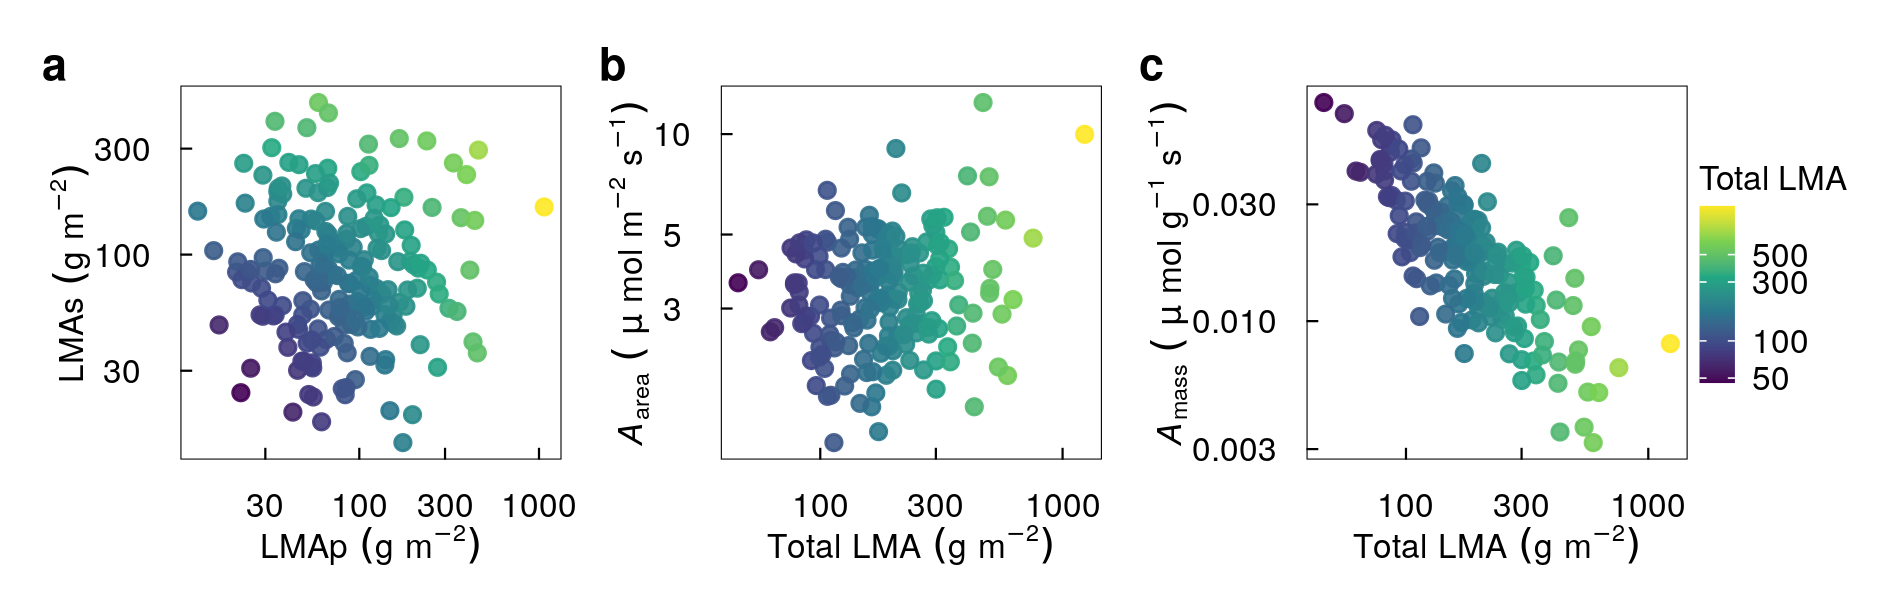
\includegraphics{/home/mattocci/LMAms/figs/hypo.png}
%DIFDELCMD < %%%
\DIFdelendFL \DIFaddbeginFL [} \DIFaddFL{Simulated two-dimensional functional space that can result in
either a two- or one-dimensional trait space, depending on how metabolic
traits are normalized. (a) Hypothetical independent variation in two
leaf mass per area (LMA) components: metabolic leaf mass per area (LMAm,
which largely determines per-area values of photosynthesis, respiration,
and nutrient concentrations) and structural leaf mass per area (LMAs,
which determines leaf toughness but has little effect on metabolic
traits). Panels b and c represent normalization by leaf area and leaf
mass, respectively. (b) Two-dimensional relationship between
photosynthetic capacity (}\emph{\DIFaddFL{A}}\DIFaddFL{\textsubscript{max}) per-unit leaf area
and total LMA (equal to LMAm + LMAs). (c) One-dimensional relationship
between }\emph{\DIFaddFL{A}}\DIFaddFL{\textsubscript{max} per-unit leaf mass and total LMA.
Methods used to simulate the data are explained in SI.
}\DIFaddendFL 

\DIFaddbeginFL \DIFaddFL{The natural logarithm of LMAm and LMAs are simulated from a hypothetical
scenario of normal distributions with means of 56 and 61 and standard
deviations of 0.83 and 1.0, and zero covariance. Variation in
}\emph{\DIFaddFL{A}}\DIFaddFL{\textsubscript{max} values are derived from our analysis of the
GLOPNET database.
\(\mathrm{ln\;} A_{\mathrm{area} \, i}= \mathrm{ln\;} 1.77 + 0.28 \; \mathrm{ln\; LMAm}_i -0.13 \; \mathrm{ln\; LMAm} + \epsilon_i\),
where \(\epsilon_i\) is normally distributed with mean 0 and standard
deviation 0.31 (see Methods and Results).
}{]\DIFaddendFL }\DIFaddbeginFL \DIFaddFL{(/Users/mattocci/Dropbox/MS/LMAms/figs/hypo.png)\{\#fig-hypo\}
}\DIFaddendFL 

\DIFdelbeginFL %DIFDELCMD < \caption{%
{%DIFAUXCMD
%DIFDELCMD < \label{fig-Hplt}%%%
\DIFdelFL{Example of a two-dimensional functional space
that can result in either a two- or one-dimensional trait space,
depending on how metabolic traits are normalized. (A) Hypothetical
independent variation in two leaf mass per area (LMA) components:
metabolic leaf mass per area (LMAp, which largely determines per-area
values of photosynthesis, respiration, and nutrient concentrations) and
structural leaf mass per area (LMAs, which determines leaf toughness but
has little effect on metabolic traits). (B) Two-dimensional relationship
between photosynthetic capacity (}\emph{\DIFdelFL{A}}%DIFAUXCMD
\DIFdelFL{\textsubscript{max}) per-unit
leaf area and total LMA (equal to LMAp + LMAs). (C) One-dimensional
relationship between }\emph{\DIFdelFL{A}}%DIFAUXCMD
\DIFdelFL{\textsubscript{max} per-unit leaf mass and
total LMA. LMAp and LMAs are simulated from a hypothetical scenario of
lognormal distributions with medians of 80 and standard deviations of
exp(0.8) and exp(0.7), and zero covariance. Variation in
}\emph{\DIFdelFL{A}}%DIFAUXCMD
\DIFdelFL{\textsubscript{max} values are derived from our analysis of the
GLOPNET database.
\(A_{\mathrm{area} \, i}=1.81 \times \mathrm{LMAp}_i^{0.28}\mathrm{LMAs}^{-0.13}\epsilon_i\),
where \(\epsilon_i\) is log-normally distributed with log-mean with 0,
log-scale parameter with 0.31 (see Methods and Results).}}
%DIFAUXCMD
%DIFDELCMD < 

%DIFDELCMD < \end{figure}
%DIFDELCMD < 

%DIFDELCMD < %%%
\DIFdelend \begin{figure}

{\centering \DIFdelbeginFL %DIFDELCMD < \includegraphics{/home/mattocci/LMAms/figs/gl_point.png}
%DIFDELCMD < %%%
\DIFdelendFL \DIFaddbeginFL \includegraphics{/Users/mattocci/Dropbox/MS/LMAms/figs/gl_point.png}
\DIFaddendFL 

}

\caption{\DIFdelbeginFL %DIFDELCMD < \label{fig-GLplt}%%%
\DIFdelendFL \DIFaddbeginFL \label{fig-gl_point}\DIFaddendFL Observed and estimated leaf-trait
relationships in the global GLOPNET dataset. Estimates are from \DIFdelbeginFL \DIFdelFL{Model 2b
}\DIFdelendFL \DIFaddbeginFL \DIFaddFL{the best
GLOPNET model }\DIFaddendFL (Table 1). Leaf life span (LL), net photosynthetic rate
per unit leaf area (\emph{A}\textsubscript{area}), and dark respiration
rate per unit leaf area (\emph{R}\textsubscript{area}) are plotted
against observed LMA, posterior \DIFdelbeginFL \DIFdelFL{means }\DIFdelendFL \DIFaddbeginFL \DIFaddFL{medians }\DIFaddendFL of \DIFdelbeginFL \DIFdelFL{LMAp }\DIFdelendFL \DIFaddbeginFL \DIFaddFL{LMAm }\DIFaddendFL and LMAs. Pearson
correlation coefficients (\emph{r}) for LMA (left column) and posterior
\DIFdelbeginFL \DIFdelFL{means }\DIFdelendFL \DIFaddbeginFL \DIFaddFL{medians }\DIFaddendFL of Pearson correlation coefficients (\(\bar{r}\)) or partial
correlation coefficients (\(\bar{\rho}\)) \DIFdelbeginFL \DIFdelFL{of LMAp }\DIFdelendFL \DIFaddbeginFL \DIFaddFL{for LMAm }\DIFaddendFL (middle column) and
LMAs (right column) are shown. Note that LL was modeled by LMAs alone
\DIFaddbeginFL \DIFaddFL{due to improved model performance with this parameter constraint (Table
1)}\DIFaddendFL . \DIFaddbeginFL \DIFaddFL{Therefore, (\(\bar{r}\)) is reported for LL (single predictor
variable), whereas (\(\bar{\rho}\)) is reported for
}\emph{\DIFaddFL{A}}\DIFaddFL{\textsubscript{area} and }\emph{\DIFaddFL{R}}\DIFaddFL{\textsubscript{area} (multiple
predictor variables).}\DIFaddendFL }

\end{figure}

\newpage

\begin{figure}

{\centering \DIFdelbeginFL %DIFDELCMD < \includegraphics{/home/mattocci/LMAms/figs/pa_point.png}
%DIFDELCMD < %%%
\DIFdelendFL \DIFaddbeginFL \includegraphics{/Users/mattocci/Dropbox/MS/LMAms/figs/pa_point.png}
\DIFaddendFL 

}

\caption{\DIFdelbeginFL %DIFDELCMD < \label{fig-PAplt}%%%
\DIFdelendFL \DIFaddbeginFL \label{fig-pa_point}\DIFaddendFL Observed and estimated leaf-trait
relationships in the Panama dataset. Estimates are from \DIFdelbeginFL \DIFdelFL{Model 4a }\DIFdelendFL \DIFaddbeginFL \DIFaddFL{the best Panama
model }\DIFaddendFL (Table 1)\DIFaddbeginFL \DIFaddFL{, which included effects of light on LL}\DIFaddendFL . Details as \DIFdelbeginFL \DIFdelFL{in }\DIFdelendFL \DIFaddbeginFL \DIFaddFL{for
}\DIFaddendFL Fig.~\DIFdelbeginFL \DIFdelFL{\ref{fig-GLplt}}\DIFdelendFL \DIFaddbeginFL \DIFaddFL{\ref{fig-gl_point}}\DIFaddendFL . \DIFdelbeginFL \DIFdelFL{Results for other LL models are
summarized in Table SX. }\DIFdelendFL Note that \emph{A}\textsubscript{area} and LL
were modeled by \DIFdelbeginFL \DIFdelFL{LMAp }\DIFdelendFL \DIFaddbeginFL \DIFaddFL{LMAm }\DIFaddendFL and LMAs alone, respectively\DIFaddbeginFL \DIFaddFL{, due to improved model
performance with these parameter constraints (Table 1)}\DIFaddendFL . \DIFaddbeginFL \DIFaddFL{The results
shown here include all leaves in the Panama dataset. The observed
separation of LL between sun and shade leaves is accounted for in the
model predictions Fig.~\ref{fig-ll_point}.}\DIFaddendFL }

\end{figure}

\newpage

\begin{figure}

{\centering \DIFdelbeginFL %DIFDELCMD < \includegraphics{/home/mattocci/LMAms/figs/pa_point_par_ll.png}
%DIFDELCMD < %%%
\DIFdelendFL \DIFaddbeginFL \includegraphics{/Users/mattocci/Dropbox/MS/LMAms/figs/pa_point_par_ll.png}
\DIFaddendFL 

}

\caption{\DIFdelbeginFL %DIFDELCMD < \label{fig-LLplt}%%%
\DIFdelendFL \DIFaddbeginFL \label{fig-ll_point}\DIFaddendFL Relationship between \DIFdelbeginFL \DIFdelFL{residuals of }\DIFdelendFL leaf lifespan (LL) \DIFdelbeginFL \DIFdelFL{against light }\DIFdelendFL and
\DIFdelbeginFL \DIFdelFL{residuals of }\DIFdelendFL LMAs \DIFdelbeginFL \DIFdelFL{against }\DIFdelendFL \DIFaddbeginFL \DIFaddFL{in the Panama dataset, after accounting for the effects of }\DIFaddendFL light
\DIFaddbeginFL \DIFaddFL{(suv vs}\DIFaddendFL .\DIFaddbeginFL \DIFaddFL{~shade leaves; see Eq. 4b). }\DIFaddendFL The dashed line indicates the 1:1
relationship \DIFaddbeginFL \DIFaddFL{expected for residuals on the log-scale}\DIFaddendFL . The posterior
\DIFdelbeginFL \DIFdelFL{means }\DIFdelendFL \DIFaddbeginFL \DIFaddFL{medians }\DIFaddendFL of the partial correlation coefficient (\(\bar{\rho}\)) is
shown. \DIFaddbeginFL \DIFaddFL{The results shown here include all leaves in the Panama dataset.}\DIFaddendFL }

\end{figure}

\newpage

\begin{figure}

{\centering \DIFdelbeginFL %DIFDELCMD < \includegraphics{/home/mattocci/LMAms/figs/vpart_intra.png}
%DIFDELCMD < %%%
\DIFdelendFL \DIFaddbeginFL \includegraphics{/Users/mattocci/Dropbox/MS/LMAms/figs/vpart_intra.png}
\DIFaddendFL 

}

\caption{\label{fig-vpart}Variance partitioning on LMA components
between and within leaf habits (evergreen vs.~\DIFdelbeginFL \DIFdelFL{deciuous}\DIFdelendFL \DIFaddbeginFL \DIFaddFL{deciduous}\DIFaddendFL ) for the GLOPNET
dataset and the Panama dataset, and between and within sites (wet
vs.~dry) and light (sun vs.~shade) for the Panama dataset. \DIFaddbeginFL \DIFaddFL{To isolate
the effects of intraspecific variation, the Panama results shown here
only include species for which both sun and shade leaves were
available.}\DIFaddendFL }

\end{figure}

\newpage

\begin{figure}

{\centering \DIFdelbeginFL %DIFDELCMD < \includegraphics{/home/mattocci/LMAms/figs/box_de.png}
%DIFDELCMD < %%%
\DIFdelendFL \DIFaddbeginFL \includegraphics{/Users/mattocci/Dropbox/MS/LMAms/figs/box_de.png}
\DIFaddendFL 

}

\caption{\DIFdelbeginFL %DIFDELCMD < \label{fig-boxplt_de}%%%
\DIFdelendFL \DIFaddbeginFL \label{fig-box_de}\DIFaddendFL Boxplots comparing leaf mass per area (LMA)
and posterior medians of photosynthetic and structural LMA components
(\DIFdelbeginFL \DIFdelFL{LMAp }\DIFdelendFL \DIFaddbeginFL \DIFaddFL{LMAm }\DIFaddendFL and LMAs, respectively) across deciduous (\DIFdelbeginFL \DIFdelFL{D}\DIFdelendFL \DIFaddbeginFL \DIFaddFL{Dev}\DIFaddendFL ) and evergreen (\DIFdelbeginFL \DIFdelFL{E}\DIFdelendFL \DIFaddbeginFL \DIFaddFL{Eve}\DIFaddendFL )
leaves in the GLOPNET dataset (a) and in the Panama dataset (b). The
center line in each box indicates the median, upper and lower box edges
indicate the interquartile range, whiskers show 1.5 times the
interquartile range, and points are outliers. Groups sharing the same
letters are not significantly different (P \textgreater{} 0.05;
t-tests). \DIFdelbeginFL \DIFdelFL{To isolate the effects of intraspecific variation (i.e.,
plastic responses to light), the }\DIFdelendFL \DIFaddbeginFL \DIFaddFL{The }\DIFaddendFL Panama results \DIFdelbeginFL \DIFdelFL{shown here }\DIFdelendFL only include species for which both sun and
shade leaves were available\DIFdelbeginFL \DIFdelFL{(}\textbf{\DIFdelFL{revise this text}}%DIFAUXCMD
\DIFdelFL{)}\DIFdelendFL . Qualitatively similar results were obtained
when all Panama species were included (Fig. \DIFdelbeginFL \DIFdelFL{S\ref{fig-box_inter}}\DIFdelendFL \DIFaddbeginFL \DIFaddFL{S1}\DIFaddendFL ). Note that the vertical
axis is on a log\textsubscript{10} scale.}

\end{figure}

\newpage

\begin{figure}

{\centering \DIFdelbeginFL %DIFDELCMD < \includegraphics{/home/mattocci/LMAms/figs/box_pa.png}
%DIFDELCMD < %%%
\DIFdelendFL \DIFaddbeginFL \includegraphics{/Users/mattocci/Dropbox/MS/LMAms/figs/box_pa.png}
\DIFaddendFL 

}

\caption{\DIFdelbeginFL %DIFDELCMD < \label{fig-boxplt_pa}%%%
\DIFdelendFL \DIFaddbeginFL \label{fig-box_pa}\DIFaddendFL Boxplots comparing leaf mass per area (LMA)
and posterior medians of \DIFdelbeginFL \DIFdelFL{photosynthetic }\DIFdelendFL \DIFaddbeginFL \DIFaddFL{metabolic }\DIFaddendFL and structural LMA components (\DIFdelbeginFL \DIFdelFL{LMAp }\DIFdelendFL \DIFaddbeginFL \DIFaddFL{LMAm
}\DIFaddendFL and LMAs, respectively\DIFaddbeginFL \DIFaddFL{) }\DIFaddendFL across sites (wet and dry) and canopy strata
(sun and shade) in the Panama dataset\DIFdelbeginFL \DIFdelFL{(bottom)}\DIFdelendFL . \DIFdelbeginFL \DIFdelFL{To isolate
the effects of intraspecific variation (i.e., plastic responses to
light), the Panama }\DIFdelendFL \DIFaddbeginFL \DIFaddFL{These }\DIFaddendFL results \DIFdelbeginFL \DIFdelFL{shown here }\DIFdelendFL only include
species for which both sun and shade leaves were available.
Qualitatively similar results were obtained when all Panama species were
included (Fig. \DIFdelbeginFL \DIFdelFL{S\ref{fig-box_inter}}\DIFdelendFL \DIFaddbeginFL \DIFaddFL{S1}\DIFaddendFL ). Details as for Fig.~\DIFdelbeginFL \DIFdelFL{\ref{fig-boxplt_de}}\DIFdelendFL \DIFaddbeginFL \DIFaddFL{\ref{fig-box_de}.}\DIFaddendFL }

\end{figure}

\newpage

\begin{figure}

{\centering \DIFdelbeginFL %DIFDELCMD < \includegraphics{/home/mattocci/LMAms/figs/mass_prop_mv.png}
%DIFDELCMD < %%%
\DIFdelendFL \DIFaddbeginFL \includegraphics{/Users/mattocci/Dropbox/MS/LMAms/figs/mass_prop_mv.png}
\DIFaddendFL 

}

\caption{\DIFdelbeginFL %DIFDELCMD < \label{fig-massplt}%%%
\DIFdelFL{The relationships }\DIFdelendFL \DIFaddbeginFL \label{fig-mass_prop}\DIFaddFL{Relationships }\DIFaddendFL between mass dependency
(\emph{b} in Eq. \DIFdelbeginFL \DIFdelFL{~\ref{eq-var}}\DIFdelendFL \DIFaddbeginFL \DIFaddFL{5}\DIFaddendFL ) and \DIFdelbeginFL \DIFdelFL{relative variance in }\DIFdelendFL LMAs \DIFaddbeginFL \DIFaddFL{variance (relative }\DIFaddendFL to \DIFaddbeginFL \DIFaddFL{total }\DIFaddendFL LMA \DIFaddbeginFL \DIFaddFL{variance;
Eq. 6) }\DIFaddendFL for the global \DIFdelbeginFL \DIFdelFL{GLOPNET }\DIFdelendFL \DIFaddbeginFL \DIFaddFL{GLPNET }\DIFaddendFL dataset, sun leaves in Panama, and shade
leaves in Panama. Solid lines indicate simulated \DIFdelbeginFL \DIFdelFL{means }\DIFdelendFL \DIFaddbeginFL \DIFaddFL{medians }\DIFaddendFL and shaded
regions indicate 95\% \DIFdelbeginFL \DIFdelFL{CI}\DIFdelendFL \DIFaddbeginFL \DIFaddFL{confidence intervals}\DIFaddendFL . Each \DIFdelbeginFL \DIFdelFL{symbol }\DIFdelendFL \DIFaddbeginFL \DIFaddFL{point }\DIFaddendFL indicates the
estimated values from the empirical data \DIFaddbeginFL \DIFaddFL{and represents interspecific
variation (e.g., across species within a canopy position in the Panama
dataset)}\DIFaddendFL . The \DIFaddbeginFL \DIFaddFL{y-axis values indicates if }\DIFaddendFL photosynthetic \DIFdelbeginFL \DIFdelFL{rate }\DIFdelendFL \DIFaddbeginFL \DIFaddFL{capacity
}\DIFaddendFL (\emph{A}\textsubscript{max}) is \DIFaddbeginFL \DIFaddFL{is }\DIFaddendFL primarily mass-dependent (\emph{b}
\textgreater{} 0.5) \DIFdelbeginFL \DIFdelFL{, }\DIFdelendFL \DIFaddbeginFL \DIFaddFL{or }\DIFaddendFL primarily area-dependent (0.5 \textgreater{}
\emph{b} \textgreater{} 0)\DIFdelbeginFL \DIFdelFL{and purely area-dependent
(}\DIFdelendFL \DIFaddbeginFL \DIFaddFL{, with }\DIFaddendFL \emph{b} \DIFdelbeginFL \DIFdelFL{= }\DIFdelendFL \DIFaddbeginFL \DIFaddFL{near }\DIFaddendFL 0 \DIFdelbeginFL \DIFdelFL{) }\DIFdelendFL \DIFaddbeginFL \DIFaddFL{indicating purely
area-dependendence }\DIFaddendFL (\protect\hyperlink{ref-Osnas2018}{Osnas et al.
2018}). \DIFdelbeginFL \DIFdelFL{Note that when }\DIFdelendFL \DIFaddbeginFL \DIFaddFL{If }\DIFaddendFL \emph{b} \textgreater{} 1, \DIFaddbeginFL \DIFaddFL{then }\DIFaddendFL \emph{A}\DIFdelbeginFL \DIFdelFL{\textsubscript{area}
dramatically }\DIFdelendFL \DIFaddbeginFL \DIFaddFL{\textsubscript{max}
}\DIFaddendFL increases \DIFaddbeginFL \DIFaddFL{exponentially }\DIFaddendFL with LMA, which is not \DIFdelbeginFL \DIFdelFL{realistic}\DIFdelendFL \DIFaddbeginFL \DIFaddFL{consistent with observed
relationships (}\protect\hyperlink{ref-Osnas2018}{Osnas et al. 2018}\DIFaddFL{)}\DIFaddendFL .}

\end{figure}

\newpage

\begin{figure}

{\centering \DIFdelbeginFL %DIFDELCMD < \includegraphics{/home/mattocci/LMAms/figs/pa_point_npc.png}
%DIFDELCMD < %%%
\DIFdelendFL \DIFaddbeginFL \includegraphics{/Users/mattocci/Dropbox/MS/LMAms/figs/pa_point_npc.png}
\DIFaddendFL 

}

\caption{\DIFdelbeginFL %DIFDELCMD < \label{fig-PA-NPC}%%%
\DIFdelendFL \DIFaddbeginFL \label{fig-pa_npc}\DIFaddendFL Measured traits \DIFaddbeginFL \DIFaddFL{in the Panama dataset }\DIFaddendFL related
to photosynthesis and metabolism \DIFdelbeginFL \DIFdelFL{traits }\DIFdelendFL (nitrogen and phosphorus per-unit leaf
area; \emph{N}\textsubscript{area} and \emph{P}\textsubscript{area}) are
\DIFdelbeginFL \DIFdelFL{strongly }\DIFdelendFL \DIFaddbeginFL \DIFaddFL{better }\DIFaddendFL correlated with estimates (posterior medians) of the \DIFdelbeginFL \DIFdelFL{photosynthetic }\DIFdelendFL \DIFaddbeginFL \DIFaddFL{metabolic
}\DIFaddendFL LMA component (\DIFdelbeginFL \DIFdelFL{LMAp}\DIFdelendFL \DIFaddbeginFL \DIFaddFL{LMAm}\DIFaddendFL ) \DIFaddbeginFL \DIFaddFL{than the structural component (LMAs)}\DIFaddendFL , \DIFdelbeginFL \DIFdelFL{and }\DIFdelendFL \DIFaddbeginFL \DIFaddFL{whereas the
opposite pattern occurs for }\DIFaddendFL a measured structural trait (cellulose
per-unit leaf area; \DIFdelbeginFL \emph{\DIFdelFL{CL}}%DIFAUXCMD
\DIFdelendFL \DIFaddbeginFL \DIFaddFL{CL}\DIFaddendFL \textsubscript{area})\DIFdelbeginFL \DIFdelFL{is
strongly correlated with estimates of the structural LMA component
(LMAs) for the Panama dataset}\DIFdelendFL .
\DIFdelbeginFL \DIFdelFL{Note that sun and shade leaves align
along a single relationship for }\emph{\DIFdelFL{CL}}%DIFAUXCMD
\DIFdelFL{\textsubscript{area} vs.~LMAs,
but not for }\emph{\DIFdelFL{CL}}%DIFAUXCMD
\DIFdelFL{\textsubscript{area} vs.~LMA or LMAp.
}\DIFdelendFL \emph{N}\textsubscript{area}, \emph{P}\textsubscript{area}, and
\DIFdelbeginFL \emph{\DIFdelFL{CL}}%DIFAUXCMD
\DIFdelendFL \DIFaddbeginFL \DIFaddFL{CL}\DIFaddendFL \textsubscript{area} data were not used to fit the models, and are
presented here as independent support for the model results. Pearson
correlation coefficients (\emph{r}) for LMA \DIFdelbeginFL \DIFdelFL{(left column) }\DIFdelendFL and \DIFdelbeginFL \DIFdelFL{partial
}\DIFdelendFL \DIFaddbeginFL \DIFaddFL{the posterior medians of
Pearson }\DIFaddendFL correlation coefficients (\DIFdelbeginFL \DIFdelFL{\(\rho\)}\DIFdelendFL \DIFaddbeginFL \DIFaddFL{\(\bar{r}\)}\DIFaddendFL ) \DIFdelbeginFL \DIFdelFL{of LMAp (middle column) }\DIFdelendFL \DIFaddbeginFL \DIFaddFL{for LMAm }\DIFaddendFL and LMAs \DIFdelbeginFL \DIFdelFL{(right column) }\DIFdelendFL are
shown. Analogous results were obtained for \emph{N}\textsubscript{area}
and \emph{P}\textsubscript{area} for GLOPNET (Fig. \DIFdelbeginFL \DIFdelFL{S\ref{fig-glnp}}\DIFdelendFL \DIFaddbeginFL \DIFaddFL{S6}\DIFaddendFL ). \DIFdelbeginFL \DIFdelFL{Results for other LL models are reported
in Table SX. Analogous }\DIFdelendFL \DIFaddbeginFL \DIFaddFL{The }\DIFaddendFL results
\DIFdelbeginFL \DIFdelFL{were obtained }\DIFdelendFL \DIFaddbeginFL \DIFaddFL{shown here include all leaves }\DIFaddendFL for \DIFaddbeginFL \DIFaddFL{which }\DIFaddendFL \emph{N}\textsubscript{area}\DIFdelbeginFL \DIFdelFL{and }\DIFdelendFL \DIFaddbeginFL \DIFaddFL{,
}\DIFaddendFL \emph{P}\textsubscript{area} \DIFdelbeginFL \DIFdelFL{for
GLOPNET (Fig. S\ref{fig-glnp})}\DIFdelendFL \DIFaddbeginFL \DIFaddFL{and CL\textsubscript{area} are available}\DIFaddendFL .}

\end{figure}



\end{document}
